% add pdflatex cue for arxiv submission
\pdfoutput=1
% -*- TeX -*- -*- Soft -*-
%Daemon> filter=err+warn
%Daemon> ini=pdflatex
%Daemon> aux-directory=TexAux
%Daemon> custom_args="-synctex=1"
%%Daemon> custom_args="-synctex=1 -enable-installer"


%\documentclass{article}

% See https://www.elsevier.com/__data/assets/pdf_file/0009/56844/elsdoc2.pdf

\documentclass{elsarticle}


\usepackage[titletoc]{appendix}
\usepackage{etex,etoolbox}
\usepackage{lscape}
\usepackage{amsmath, amsthm, amssymb}
\usepackage{gamesem}
\usepackage{pst-tree}
\usepackage[inline]{enumitem}
\usepackage{pstring}
\usepackage{xspace}
\usepackage{todonotes}
\usepackage{amsmath,amssymb,amsthm}
\usepackage{bcprules}
\usepackage{algorithm}
\usepackage{algorithmic}
\usepackage{geometry}
\usepackage{pdflscape}
\usepackage{multirow}
\usepackage{subcaption}
\usepackage{tcolorbox}
\usepackage{wrapfig}
\usepackage{url}
%\usepackage{halloweenmath}
\usetikzlibrary{arrows,automata}


\newif\ifshortversion
\newif\iflongversion

\shortversiontrue

\ifshortversion
\longversionfalse
\else
\longversiontrue
\fi


% Markers used for proof only included in the short version of the paper
\ifshortversion
\def\shortproof{\begin{proof}}
\def\endshortproof{\end{proof}}
\else
\long\def\shortproof#1\endshortproof{}
\fi

%%%%%%%% Inline/deferred proof macros
% Define this macro to defer complex proofs to the end of the document?
% or comment out to keep default behaviour (inline proof)
\def\placeproofsatend{}

%%%%%%%% Uncomment to include TODO boxes
\def\includetodos{}

\newtcolorbox{ruletablebox}[1]{
    %colback=red!5!white,
    colframe=blue!75!black,
    title=#1
}

\newtcolorbox{remarkbox}{
    colframe=blue!75!black
}

\ifdefined\includetodos
\newtcolorbox{todobox}{
    colback=orange!5!white,
    colframe=orange!75!black,
    title=TODO
}
\else
\newcommand\todobox[1]{}
\fi

\makeatletter
\providecommand{\@fourthoffour}[4]{#4}
% We define an addition for the theorem-like environments; when
% \newtheorem{thm}{Theorem} is declared, the macro \thm expands
% to {...}{...}{...}{Theorem} and with \@fourthoffour we access
% to it; then we make available \@currentlabel (the theorem number)
% also outside the environment.
\def\fixstatement#1{%
    \AtEndEnvironment{#1}{%
    \xdef\pat@label{\expandafter\expandafter\expandafter
        \@fourthoffour\csname#1\endcsname\space\@currentlabel}}}

% We allocate a block of 1000 token registers; in this way \prooftoks
% is 1000 and we can access the following registers of the block by
% \prooftoks+n (0<n<1000); we'll use a dedicated counter for it
% that is stepped at every proof
\globtoksblk\prooftoks{1000}
\newcounter{proofcount}

\ifshortversion
% skip all proof at end in short version of the paper
\long\def\proofatend#1\endproofatend{}
\else
\ifdefined\placeproofsatend
% Proof marked as '\proofatend' will be placed at the end of the document.
% We gather the contents of the proof as argument to \proofatend
% and then we store
% "\begin{proof}[Proof of <theoremname> <theoremnumber>]#1\end{proof}"
% in the next token register of the allocated block
\long\def\proofatend#1\endproofatend{%
    \edef\next{\noexpand\begin{proof}[Proof of \pat@label]}%
    \toks\numexpr\prooftoks+\value{proofcount}\relax=\expandafter{\next#1\end{proof}}
    \stepcounter{proofcount}}
\else
% Proof marked as '\proofatend' will instead be expanded inline
\def\proofatend{\begin{proof}}
\def\endproofatend{\end{proof}}
\fi

\fi

% \printproofs simply loops over the used token registers of the
% block, freeing their contents
\def\printproofs{%
    \count@=\z@
    \loop
    \the\toks\numexpr\prooftoks+\count@\relax
    \ifnum\count@<\value{proofcount}%
    \advance\count@\@ne
    \repeat}
\makeatother
%%%%% END OF Inline/deferred proof macros




\theoremstyle{plain}
\newtheorem{theorem}{Theorem}[section]
\newtheorem{proposition}[theorem]{Proposition}
\newtheorem{lemma}[theorem]{Lemma}
\newtheorem{corollary}[theorem]{Corollary}
\newtheorem{property}[theorem]{Property}

\theoremstyle{definition}
\newtheorem{definition}{Definition}[section]
\newtheorem{example}{Example}[section]

%\theoremstyle{remark}
%\newtheorem{remark}{Remark}[section]

\fixstatement{theorem}
\fixstatement{proposition}
\fixstatement{property}
\fixstatement{lemma}

\setlist[itemize]{itemindent=0.3em}
\setlist[description]{itemindent=0.2em}

% Change the numbering used for Algorithms
\renewcommand*{\thealgorithm}{\Alph{algorithm}}
\renewcommand{\algorithmicrequire}{\textbf{Input:}}
\renewcommand{\algorithmicensure}{\textbf{Output:}}

% Set of variable occurrences of a term
\newcommand\VarOcc{\mathcal{O}{cc}}
% set of variable identifiers
\newcommand\VarSet{\mathcal{V}}
\newcommand\Nodes{\mathcal{N}}% set of structural nodes of the tree
\newcommand\NodesVar{\Nodes_{\sf var}}% set of variable  nodes
\newcommand\NodesLmd{\Nodes_\lambda}% set of lambda nodes
\newcommand\NodesApp{\Nodes_@}% set of application nodes

\newcommand{\ghostlmd}{{\lambda\mkern-7mu \lambda}}
%\newcommand{\ghostvar}{\theta}
%\newcommand{\ghostvar}{{\mathghost}}
%\newcommand{\ghostvar}{\mathsf{x\!\!x}}
\newcommand{\ghostvar}{\mathsf{x\mkern-5mu x}}




% set of nodes of the extensional tree
% (= structural + ghost nodes)
\newcommand\ExtendedNodes{\tilde{\Nodes}}
% set of extended variable nodes = structural + ghost variable nodes
\newcommand\ExtendedNodesVar{\tilde{\Nodes}_{\sf var}}
% set of extended lambda nodes = structural + ghost lambda nodes
\newcommand\ExtendedNodesLmd{\tilde{\Nodes}_{\lambda}}


\newcommand{\normalizing}{{\sf norm}}
\newcommand{\essential}{{\sf ess}}
\newcommand{\concrete}{{\sf con}}
\newcommand{\concreteessential}{{\sf c.e.}}

\newcommand\travsetshort{\mathcal{T}\!r}
\newcommand{\travsetes}{{\travset_\essential}} % essential traversals
\newcommand{\travsetcon}{{\travset_\concrete}} % concrete traversals
\newcommand{\travsetcones}{\travset_\concreteessential} % concrete and essential traversals
\newcommand{\travsetnorm}{\travset_\normalizing} % normalizing traversals
\newcommand{\travsetscn}{\travset_{\sf c.s.n.}} % complete-strand normalizing traversals

\def\almostequal{\doteq}  % almost justified sequence equality
%\def\almosteqisomorphic{\stackrel{.}{\cong}} % almost-equal isomorphism
\def\structisomorphic{\cong} % structural-equality isomorphism


% for succinctness we omit ULC for the symbol representing
% set of traversals of ULC
% (this is not ambiguous since ULC and STLC are shown to coincide in this paper)
\newcommand{\travulc}{\travset}


\newcommand{\child}{{\small \sf Ch}} % unique child of a node

\newcommand{\rulefont}[1]{\mathbf{\sf #1}}

\def\readout{\mathrm{R}} % readout function

\def\coresymbol{\pi} % function returning the core of a traversal
\newcommand{\core}[1]{\coresymbol(#1)} % core of a traversal

\def\nameencoding{\mathcal{E}} % name-preserving encoding


\DeclareMathSymbol{\Tau}{\mathalpha}{operators}{"54}

\newcommand{\enables}{\vdash} %enabling relation
\newcommand{\ctree}{\Tau} % tree of a term
\newcommand{\exttree}{\tilde{\Tau}} % extensional tree with ghost nodes

% Set of external nodes = nodes hereditarily justified by the root
\newcommand{\ExternalNodes}{\Nodes^{\sf ext}}

% Set of internal nodes = nodes hereditarily justified by @-nodes
\newcommand{\InternalNodes}{\Nodes^{\sf int}}

\newcommand\pathset{{\mathcal{P}aths}} % set of paths in the comp tree
\newcommand\dynar{\textsf{dynar}} % dynamic arity

\renewcommand\ie{{\it i.e.\@\xspace}}
\renewcommand\eg{{\it e.g.\@\xspace}}

% partial function definition
\newcommand\pfun{\mathrel{\ooalign{\hfil$\mapstochar\mkern5mu$\hfil\cr$\to$\cr}}}

% Bulk lambda abstraction of a sequence of variables
\newcommand\bulklambda[1]{{\lambda\overline{#1}}}

% et al
\def\etal{\textit{et al.}\@\xspace}

% head linear reduction
\newcommand{\hlred}{\rightarrow_{hl}}

% leftmost linear reduction
\newcommand{\llred}{\rightarrow_{ll}}

% head variable occurrence (from Danos-Regnier def)
\newcommand{\hoc}{\emph{hoc}}

% Term equivalence up to alpha renaming
%\newcommand{\alphaequiv}{\equiv}

% set of justified sequences of M
\def\justseqset{\mathcal{J}}
\def\istraversal{\models}

\author{William Blum}
\ead{william.blum@microsoft.com}
\address{Microsoft Research, One Microsoft Way, Redmond, WA, 98052, USA}

\title{Evaluating Lambda Terms with Traversals
\\ \vspace*{1em}
\today}
% Traversing And Evaluating Untyped Lambda Terms(preprint)
% Traversal-based Evaluation of Untyped Lambda Terms (preprint)
% Traversing Untyped Lambda Term
% Traversal Theory of the Untyped Lambda Calculus
% Imaginary Traversals of Untyped Lambda Terms
% Reducing Lambda Terms with Imaginary Traversals (preprint)
% Reduction of Untyped Lambda Terms by Imaginary Traversals
% Normalizing Untyped Lambda Terms via Imaginary Traversals
% Imaginary Normalizing Traversals
% Imaginary Traversals and Leftmost Linear Reduction
% Normalizing Lambda Terms via Imaginary Traversals and Leftmost Linear Reduction
% Normalizing Lambda Terms via Traversals and on-the-fly eta-expansion
% Normalizing Lambda Terms with Imaginary Traversals


\begin{document}

%%%%%% A longer abstract
%%%%%%
% \begin{abstract}
%     We introduce a method to evaluate untyped lambda terms by combining the theory of traversals, a term-tree traversing technique inspired by Game Semantics~\cite{OngLics2006,BlumPhd}, with judicious use of the eta-conversion rule of the lambda calculus.

%     The traversal theory of the simply-typed lambda calculus relies on the eta-long transform to ensure that when traversing an application, there exists a subterm representing every possible operator's argument~\cite{BlumPhd, OngLics2006}. In the untyped setting, we instead exhibit the missing operand via ad-hoc instantiation of the eta-expansion rule, which allows the traversal to proceed as if the operand existed in the original term. This gives rise to a more generic concept of traversals for lambda terms where no preliminary transformation is required: the original unaltered lambda term is traversed.

%     %Blindly applying the rules of typed traversals on untyped terms, where eta-long transform is undefined, therefore fails when an operator  node lacks the required operand. To work around this limitation, we create missing operands on-the-fly and proceed as if it existed in the original term. We denote missing operands in the traversals using ``imaginary'' nodes representing nodes that would exist in the term-tree if the application subterm lacking the operand were to be eta-expanded. We call the resulting traversal an ``imaginary traversal''.

%     We show that by bounding the non-determinism of the traversal rule for free variables, one can effectively compute a set of traversals characterizing the paths in the tree representation of the beta-normal form, when it exists. This yields an evaluation algorithm for untyped lambda-terms. We prove correctness by showing that traversals implement \emph{leftmost linear reduction}, a generalization of the \emph{head linear reduction} of Danos~\etal \cite{danos-head,danosherbelinregnier1996}.
% \end{abstract}


\begin{abstract}
    A method to evaluate untyped lambda terms based on a term-tree traversing technique inspired by Game Semantics and the judicious use of eta-expansion.
    As \emph{traversals} explore nodes of the term tree,
    some of the subterms are dynamically eta-expanded in order to locate their non-immediate arguments.
    A quantity called \emph{dynamic arity} determines the necessary amount of
    eta-expansion to perform at a given point in a traversal.
    The resulting traversals are finitely enumerable and characterize the paths in the tree representation of the beta-normal form when it exists.
    Correctness of the evaluation method follows from
    the fact that traversals implement \emph{leftmost linear reduction}, a non-standard reduction strategy based on \emph{head linear reduction} of Danos-Regnier.
\end{abstract}

\maketitle

%\tableofcontents

\section{Introduction}

\subsection{Background}
The theory of traversals was originally introduced in the context of tree generating higher-order recursion schemes~\cite{OngLics2006} and was
then extended to simply-typed languages with higher-order free variables, such as the simply-typed lambda calculus (STLC)~\cite{BlumPhd}. A traversal consists of a sequence of nodes taken from a tree-representation of the \emph{eta-long expanded} term, where every node occurrence may have an associated labelled link, or ``justification pointer'', referring to some previous occurrence in the sequence. It always starts from the root of the tree and successively visits other nodes by either descending deeper into the tree structure or jumping to other tree branches. A small set of rules formally defines how to extend a given traversal--what node to visit next with which justification pointer. This yields a prefix-closed set of justified sequences of nodes defining the set of traversals of the term.

In the typed setting, the traversal theory bears a strong connection with Game Semantics~\cite{BlumPhd}: The game denotation of an eta-long term is in bijection with the set of \emph{core projections} of its traversals (Theorem~\ref{thm:gamesem_correspondence_stlc}), where the core projection of a traversal is the subsequence obtained by keeping only occurrences that are
transitively justified by the initial node.
The set of traversals itself, on the other hand, corresponds to the game semantic denotation of a term where all the internal moves are revealed, also called ``interaction game semantics''~\cite{BlumPhd}.

This correspondence gives rise to a method for finding the normal form of a simply-typed lambda term~\cite{BlumPhd,BlumGalop2008,Blum-LocalBeta2008}
where each traversal explores a branch in the tree representation of the normal form. The underlying sequences of nodes and pointers encode the unfolding of the normalization procedure over branches of the normal form. There are two kinds of nodes: the \emph{internal} nodes record intermediate steps of the reduction procedure, while \emph{external} nodes represent actual nodes from the tree representation of the normal form. The core projection performs
`garbage collection' by removing all the internal nodes from the traversals,  yielding a path in the abstract syntax tree of the normal form.


%%%%%%%%%%%%%%%
\subsection{Overview}
This paper
(i) Generalizes the notion of traversals from the typed setting, referred as `\emph{concrete traversals}', to the untyped lambda calculus (ULC), which we name `\emph{imaginary traversals}';
(ii) Introduces a method to evaluate untyped lambda terms based on enumerating traversals;
(iii) Establishes a connection between traversals and \emph{head linear reduction}.

The idea of imaginary traversals starts with the following observation:
Attempting to traverse an untyped lambda term with the
traversal rules of STLC causes the traversal to get stuck when the operator sub-term of an application has insufficiently many operands. In such a situation, there is no operand node in the term tree to traverse.
A concrete traversal of the term $M = (\lambda f.f)(\lambda x.x)$, for example,  gives the sequence of nodes $\lambda f \cdot f \cdot \lambda x \cdot x$, at which point no further node can be traversed since there is no subterm representing the first argument of $f$.
Similarly, a concrete traversal of $U = (\lambda x. x x)(\lambda y. y)$,
detailed in Example~\ref{examp:baby}, gets stuck after traversing $y$. To take an analogy with abstract machine evaluators, this would be like a broken implementation of a Krivine machine~\cite{Krivine2007} attempting to lookup a variable from an empty environment, or an SECD machine~\cite{landin-secd} attempting to pop an argument from an empty stack when evaluating the application operator.

This situation never occurs in the typed setting where lambda terms are
conveniently assumed to be \emph{eta-long expanded}, a transformation that recursively eta-expands the subterms with respect to their type,
which ensures that when traversing an application, there exists a subterm representing every possible operator's argument.
%
Untyped terms admitting a simple type, like $M$, can be traversed via eta-long expansion with respect to whichever type they inhabit.
But this is not feasible in the general ULC case where untyped terms do not necessarily inhabit a simple type.
Sometimes, well-chosen eta-expansions can help. For instance, the untyped term $U$, which has no simple type, is traversable if we eta-expand all its variable occurrences. This does not always work, unfortunately: to traverse the
term $J = (\lambda u . u(x\, u)) (\lambda v . v\, y)$ from
 Example~\ref{ex:missingoperand}, nested eta-expansions are necessary:
 the fresh variable resulting from the eta-expansion of $(x\, u)$ needs to be itself eta-expanded to unblock a concrete traversal of the term.
 Eta-expanding all variables infinitely often is not feasible, so instead imaginary traversals exhibit the missing operand via ad-hoc dynamic eta-expansion, as they traverse the term.
 This allows the traversal to proceed as if the operand existed in the original term.

So, for instance in $M$, an imaginary traversal traverses node $x$ by jumping to a fictitious fresh node $y$ that would exist if $f$ were eta-expanded
as $\lambda y.f\, y$. This trick allows the traversal to proceed with the usual traversal rules, until reaching that fictitious node $y$.
A second eta-expansion, this time of the term itself to
$\lambda z. (\lambda f y.f\, y)(\lambda x.x) z$,
unblocks the traversal, until it reaches node $z$, at which point we have a maximal traversal per the concrete traversal rules. The final traversal is given by the sequence $\lambda z \cdot @ \cdot \lambda f y \cdot f \cdot \lambda x \cdot x \cdot \lambda \cdot y \cdot \lambda \cdot z$, where `@` represents the application node in the abstract tree representation of the term, and the dummy lambda `$\lambda$' is syntactic sugar which can be ignored for now.

Generalizing this idea, we realize that concrete traversals induce an implicit `eta-expansion strategy': at any given point where a traversal gets stuck, there is only one possible subterm expansion that exhibits nodes necessary for the traversal to resume. In the term $M$, the first expansion considered is that of $f$ because, at that point, the concrete rules only let us
traverse an immediate argument of $f$. If instead we were to eta-expand the term itself, it would yield $\lambda z. (\lambda f .f)(\lambda x.x) z$
which a concrete traversal cannot traverse since $f$ does not have an immediate argument. More intuitively: at $x$ the traversal has figured out that the subterm $\lambda x.x$ should be substituted for variable $f$, therefore to determine what $x$ should be substituted for, it needs to look for the first argument of $f$. Since $f$ has no direct argument, we must eta-expand it. In this simple example, the jump into the realm of fictitious nodes is indefinite: nodes subsequently traversed are all absent from the original term. There are situations, however, such as in the term $J$, where it eventually leads to traversing an actual node from the original term tree.

In practice, it is not necessary to rewrite the term in any way in order to traverse it.
The eta-expansion occurs fictitiously and ``on the fly'' as the traversal unfolds over the original unaltered lambda term.
The ad-hoc expansion occurs when traversing a variable node, where a non-deterministic choice of `argument index' determines which variable argument to traverse next. In concrete traversals, this index is bounded by the actual number of arguments applied to the variable. In imaginary traversals, is unbounded: if it is greater than the number of static arguments applied to the variable then a fictitious eta-expansion takes place.

%%% analogy
Tree nodes resulting from such fictitious eta-expansions
are called  \emph{ghost lambda} and \emph{ghost variable} nodes.
To give an analogy, just like the imaginary number $i$ in mathematics was invented from the impossibility of calculating the square root of $-1$, we introduce ghost nodes from the impossibility of resolving the argument of a variable when traversing a lambda term: they start to appear when the arity of a variable is too low to structurally traverse it.
And just like complex numbers are sometimes used intermediately in a calculation without necessarily appearing in the final result (\eg, using De Moivre's Theorem to prove trigonometry identities on real numbers),
traversals use ghost nodes to evaluate lambda terms but they eventually materialize as regular nodes in the final normal form.
%%%%end of analogy

Evaluating an untyped term boils down to enumerating traversals.
 Although the set of imaginary traversals is infinite and the traversals  themselves can be infinitely long, we only need to consider an effectively computable subset with sufficiently enough traversals to characterize the normal form, when it exists.
We achieve this by restricting the non-determinism when traversing a variable: we bound the argument index by a critical quantity called the `dynamic arity', calculated in linear time from the traversal itself. It determines the number of arguments beyond which eta-expansions becomes unnecessary for the sake of finding a path in the normal form. This restricts both the breadth and depth of the traversal enumeration: only a finite number of on-the-fly eta-expansions are applied on a given traversal; and a traversal cannot unfold infinitely, provided that the term has a beta-normal form.
On the other hand, traversing a non-terminating term like $(\lambda x. x\,x)(\lambda x. x\,x)$ leads to infinitely long traversals, as one would expect.

The read-out phase of the algorithm appeals to a correspondence property between the traversals and paths in the tree representation of the normal form. The term $M$, for instance, has a single traversal which via suitable filtering, yields the path $\lambda z \cdot z$, therefore its beta-normal form is $\lambda z. z$, up to variable renaming.

 To prove correctness of the evaluation procedure, we show that traversals recursively implement \emph{head linear reduction}, a term reduction method
 based on a non-standard notion of redex that is reduced
 by substituting one variable occurrence at a time.

 We have implemented the evaluation procedure in HOG, a tool to study the theory of traversals and pushdown automata generated from Higher-Order Grammars and lambda terms~\cite{BlumGalop2008,Blum-HogTool}.  Section~\ref{sec:examples} includes traversals of untyped lambda terms generated with this tool.

\subsection{Related work}

\subsubsection{Theory of Traversals}

The original paper on the theory of traversals concerns higher-order recursion schemes and therefore does not deal with free variables of higher-order rank~\cite{OngLics2006}. In~\cite{BlumPhd} we extended the theory to the simply-typed lambda calculus and added traversal rule to model higher-order free variables. Both settings assume that the term or grammar is in eta-long form to guarantee that the operand of an application always exists.
In the untyped setting, eta-long expansion would be an infinite process, so instead traversals must operate on the unmodified term tree.
The present paper achieves this by eta-expanding subterms `on-the-fly' when there are insufficiently many operands in an application to continue the traversal. The term itself does not get altered: a traversal instantiates fictitious ``ghost'' nodes that would exist if the term were to be eta-expanded.
% and the traversal rules handle those fictitious nodes created in these ad-hoc eta-expansions.
When restricted to simply-typed terms, the two notions of traversal nicely coincide (Proposition~\ref{prop:ulc_and_stlc_trav_coincide}).

For simply-typed terms in eta-long form, traversals were shown to correspond to the \emph{interaction game semantic denotation}, where all internal moves from strategy composition are revealed; while the standard game denotation was shown to correspond to the set of traversals `\emph{projected with respect to the tree root}', or also called `traversal cores'. Such a correspondence induces an evaluation method for simply-typed lambda-terms in eta-long form~\cite{BlumPhd,BlumGalop2008,Ong-NormByTrav2015} that was implemented in~\cite{Blum-HogTool}, and which we state in Algorithm~\ref{algo:ulc_normalization_by_traversals}. This paper generalizes this procedure to the untyped lambda calculus, based on a variant of the traversal core operation involving relabelling of lambda nodes. A notable improvement is that it produces the traditional beta-normal form rather than the beta-\emph{eta-long} normal form. Another difference is that we prove soundness of the procedure through a connection with \emph{head-linear reduction} rather than appealing to Game Semantics.

\subsubsection{Head linear reduction}
Danos \etal established the first connection between Game Semantics and the concept of \emph{head linear reduction} for simply-typed lambda terms in eta-long form~\cite{danosherbelinregnier1996}. It was further studied in the context of untyped lambda terms~\cite{danos-head}. The \emph{pointer abstract machine} (PAM) provides a virtual machine implementation of head linear reduction that yields the ``\emph{quasi-head normal form (qhn)}'' of the term. To obtain the normal form itself, the resulting term further needs to be reduced to head normal form (via head reduction), and then normalized using standard normal reduction.

Like the PAM, the imaginary traversals implement head-linear reduction, but in a recursive fashion so as to fully evaluate the term to its final normal form.
A notion that we formalize as the \emph{leftmost linear reduction} strategy, that recursively applies head linear reduction just like how the \emph{normal reduction} of the lambda calculus proceeds by recursively applying head reduction.
A traversal starts, in a `leftmost-order'-like fashion, with a depth-first search for \emph{head occurrence} of the `\emph{hoc redex}' as defined by Danos-Regnier. It performs linear substitution by ``jumping'' to the node in the tree representing the sub-term to be substituted for that head occurrence.
To find that node, traversals implement what Danos-Regnier call ``the gymnastics to find the argument of a subterm''~\cite{danos-head} via the mechanism of `weaving' (Proposition~\ref{prop:weaving}),
where a traversal repeatedly traverses ghost lambda and variable nodes until the node representing the argument to be fetched materializes.
The link label `$|\mu|+i-|m|$' from the definition
of the lambda rule in Table~\ref{tab:trav_rules} effectively calculates the quantity $r-a+l$ that appears in step 2.(b) of the PAM transition from~\cite{danos-head}.
After performing such a jump, a traversal continues its descent to look for the next head occurrence, as if that first head occurrence had been replaced by the redex argument; until it finds the variable that will become the head variable in the normal form. At this point, a PAM would stop, whereas a traversal forks  non-deterministically and recursively traverses all possible arguments of the head variable.

A property of head-linear reduction is that all the terms appearing in the reduction sequence consist of sub-terms of the original term.
Both the PAM and traversals exploit this property via systems of pointers to avoid the traditional notions of environments or closures when (linearly) reducing a term.

\subsubsection{Berezun-Jones traversals}

Daniil Berezun and Neil Jones were first to introduce a notion of traversals for the untyped lambda calculus~\cite{JonesBerezunLLL-PEPM17}.
Although they took inspiration from the Game Semantic traversals of~\cite{OngLics2006,BlumGalop2008}, their definition is more operational in nature and does not directly relate to the game denotation of a term. Starting from operational semantics they derive a normalization method that proceeds by traversing some tree representation of the term.
%
The connection with our work lies in its correspondence with head-linear reduction: we show that imaginary traversals recursively implement head-linear reduction, and Berezun-Jones claim that a similar correspondence hold for their notion of traversal.
%
Neither notion of traversals requires any prior syntactic transformation of the input term, unlike the original traversals from the typed setting:
Their traversals operate on the traditional term tree where each node represents a token from the lambda calculus syntax,
whereas imaginary traversals operate on a compressed term tree that merges consecutive lambdas nodes and consecutive applications nodes into single bulk lambda node or bulk application node.
%
Berezun-Jones' traversals distinctively rely on two justification pointers for each token: a \emph{binding pointer} plus a \emph{control pointer}. The control pointers would be what Danos-Regnier call the ``price to pay for having no stacks or environments'' in the definition of the argument lookup transition of the Pointer Abstract Machine~\cite{danos-head}. They also involve a `flag` boolean parameter associated with every token of the traversal.
In contrast, imaginary traversals necessitate a single justification pointer per node traversed.

Another notable difference is that the normalization algorithm of Berezun-Jones requires a single traversal of the term. Our algorithm, on the other hand, produces one traversal for every possible maximal path in the tree of the beta-normal form. Each branching point in the traversal enumeration corresponds to some occurrence of a variable in the normal form, where each branch corresponds to some operand of that variable. This non-deterministic branching may conceivably be eliminated using auxiliary pointers to implement backtracking: once a variable operand is fully evaluated, the traversal would return to that variable node and start exploring remaining operands.
%
Their `read-out' procedure to reconstruct the normal form (private correspondence) involves recursively applying rewriting rules to the traversal. In contrast, our read-out algorithm reconstructs the normal form from the tree-paths induced by the maximal traversals.


\subsubsection{Lambda term evaluation}
The evaluation procedure presented in this paper contrasts with term rewriting approaches that gradually transform and refine some representation of the term until reaching a normal form. In particular, it does not involve the ``capture-avoiding'' substitution used in the standard definition of beta reduction to avoid variable capture when reducing redexes. Other reduction methods exist in the literature with the same property such as combinators, Lamping's graphs, or their variant based on the geometry of interaction~\cite{Lamping:1989:AOL:96709.96711, Gonthier:1992:GOL:143165.143172, curry_combinatorylogic, Barendregt84, the-implementation-of-functional-programming-languages}.
Just like those methods, variable names are not essential to the reduction procedure: traversals have explicit justification pointers from which variable bindings are entirely recoverable; variable names in Lamping's graphs are recoverable from their corresponding binding lambda;
Krivine and PAM machines encode names with De Bruijn indices
and combinators removes variables altogether through \emph{abstraction elimination}.
Just like graph-based reduction, the traversal evaluation procedure involves a final \emph{readback} phase to reconstruct the resulting normal form, where
all the explored paths in the term tree are assembled together to reconstruct
the normal form.
Unlike imaginary traversals, existing evaluation methods do not appeal to eta-expansion. On the other hand, they typically require transforming the term into some intermediate structure, such as a combinator expression or an interaction net, whereas traversals operate directly on the abstract syntax tree of the term.

\paragraph{GoI} The relationship of traversals with proof-nets and the Geometry of Interaction (GoI) can be seen through the lenses of head-linear reduction, which they implement, or their correspondence with game semantics. In particular, the linear substitution performed by traversals corresponds to
the firing of an exponential branch of a proof-net~\cite{MASCARI1994111}. We also point to the work of Danos and Regnier who established the connection with abstract machines and GoI~\cite{danosherbelinregnier1996}.

\subsection{Rest of the paper}

The next section introduces basic definitions from the traversal theory. Section~\ref{sec:imaginary_traversals} defines the notion of \emph{imaginary traversals} for the untyped lambda calculus. We present in Section~\ref{sec:normalizing_trav} the reduction procedure for untyped lambda terms and walk through examples in Section~\ref{sec:examples}. In Section~\ref{sec:leftmostlinearred}, we present \emph{head linear} and \emph{leftmost linear reduction}. Finally, Section~\ref{sec:correctness_ulc_normalization} shows correctness of the evaluation procedure.


\section{Terms, trees and justified sequences}
\label{sec:basic_def}
\subsection{Notations}
\emph{Sequences:} For any alphabet $\Sigma$ we write $\Sigma^*$ for the
set of (possibly infinite) sequences over elements of $\Sigma$.
 We use the abbreviation $\overline{x}$ for the sequence of elements $x_1 \ldots x_n$ for some $n\geq0$, $\epsilon$ for the empty sequence, and for any two sequences $\overline{x}, \overline{y}$ of length $n,m\geq 0$, we write $\overline{x} \cdot \overline{y}$ for the concatenation $x_1 \ldots x_n y_1 \ldots y_m$. We write $|s|$ for the length of a sequence $s$.

 \emph{Labelled trees:} Given a set of labels $\mathcal{L}$, the expression `$l\langle t_1, \ldots, t_m \rangle$' for $m \geq 0$ denotes a $\mathcal{L}$-labelled tree with root labelled $l\in \mathcal{L}$. The case $m=0$ represents a leaf-node, and for $m>0$ a node labelled $l$ with $m$ ordered children trees $t_1$, \ldots, $t_m$.
 We refer to them as the \emph{set of nodes} of the tree equipped with
 the natural parent-child relation induced by the above definition.
 %
 The maximal directed paths $\Pi(t)$ of a $\mathcal{L}$-labelled-tree $t$ are the sequences over $\mathcal{L} + \nat$
 inductively defined as
 $\Pi(l \langle t_1, \ldots t_m \rangle) = \{ l \cdot i \cdot p \ |  \ p \in \Pi(t_i), 1\leq i \leq m \}$ and
 $\Pi(l\langle \rangle) = \{ l \}$.
 The paths of a $\mathcal{L}$-labelled-tree $t$ are the odd-prefixes of its maximal paths.

\subsection{Lambda calculus background and notations}
\label{sec:lambdacalculus_basics}

We consider the set of terms $\Lambda$ of the untyped lambda calculus (ULC) constructed from the grammar $\Lambda := x\ |\ (\Lambda\, \Lambda)\ |\ \lambda x. \Lambda $
where $x$ ranges over a countable set of variable names $\VarSet$.
% countable is important so that we can pick as many fresh variables as needed
For conciseness we abbreviate consecutive lambda abstractions when writing lambda terms, so that $\lambda x_1 \ldots \lambda x_n . M$ for some $n\geq 0$ and term $M$ will be written $\lambda x_1 \ldots x_n . M$; or just
$\lambda \overline{x} . M$ if $\overline{x} = x_1 \ldots x_n$.
We will also drop brackets, and assume left-associative application so that $U\,V\,W$ means $(U\,V)\,W$. We says that two terms are $\alpha$-equivalent if they are equal up to variable renaming.
In the rest of the paper, we use uppercase letters $M, N, T, U, V$ for lambda terms and lowercase $x,y,z$ to denote variable names. Terms will all have variable names ranging in some fixed set $\VarSet$ of identifiers.

We recall standard results of the lambda calculus.
A \defname{redex} is a sub-term of the form $(\lambda x. M) N$.
Reducing redex $(\lambda x. M) N$, or also \emph{firing} the redex, means substituting all free occurrences of $x$ in $M$ by the term $N$
using capture-avoiding substitution (the bound variable is renamed afresh when recursively substituting under a lambda).
A term is said to be in \defname{$\beta$-normal form}, abbreviated $\beta$-nf, if it does not contain any redex.
A term is in \defname{head normal form} if it can be written $\lambda x_1 \ldots x_n . y A_1 \ldots A_m$ for $n,m\geq0$. If a term is not in head normal form then its \defname{head beta-redex} is the left-most redex, otherwise the term does not have any head beta-redex. For any reduction relation $\rightarrow$ between terms we will write $\rightarrow^*$ to denote its reflexive transitive closure. The \defname{eta-expansion} of $M$ refers to some term $\lambda x. M x $ for some variable $x$ fresh in $M$.

The \defname{head reduction}, denoted $\rightarrow_{h}$, fires the head redex of a term if it exists. It can be shown that $\rightarrow^*_{h}$ yields the head-normal form. The \defname{normal-order reduction strategy}, also called leftmost-outermost reduction strategy, performs head reduction until reaching the head-normal form and then recursively applies head reduction on each operand of the head variable. A standard result is that this reduction strategy yields the normal form if it exists.

\paragraph{Types} Simple types are generated from the grammar $\tau := o\, | \tau \rightarrow \tau$ where $o$ ranges over a fixed set of atomic types. Typed-annotated lambda-terms are generated from the grammar $E := \VarSet\, |\, (E\, E)\, |\, \lambda \VarSet \colon\tau. E $.
We write $M^\tau$ to denote a closed (\ie, no free variable)
type-annotated lambda-term of type $\tau$, typable with the judgment rules of the simply-typed lambda calculus~\cite{Barendregt84} and $M$ to denote the untyped term obtained by erasing its type annotations.

\subsection{Term tree and enabling relation}

We define a tree representation for untyped lambda terms where consecutive lambda abstractions are merged into a single `bulk' lambda-node and consecutive applications are represented by a single application node whose first child represents the operator, and subsequent children represent the operands.
This definition is similar to that of \emph{computation tree} from \cite{OngLics2006, BlumPhd} with the notable difference that we do not eta-long expand the term prior to constructing the tree.
\begin{definition}
The \defname{tree} $\ctree(M)$ of an
 untyped lambda term $M$ is a $\mathcal{L}$-labelled tree
with labels
$\mathcal{L} = \{ @ \} \union \VarSet \union \{ \lambda x_1 \ldots x_n \ | \ x_1 ,\ldots, x_n \in
    \VarSet, n\in\nat \}$
defined inductively by:
\begin{align*}
    \ctree(\lambda \overline{x} . z s_1 \ldots s_m) &= \lambda \overline{x}\; \langle\; z\; \langle \ctree(s_1),\ldots,\ctree(s_m)\rangle\rangle
&    \hbox{for $m\geq 0$, $z \in \VarSet$},
\\
\ctree(\lambda \overline{x} . (\lambda y.t) s_1 \ldots s_m) &= \lambda \overline{x}\; \langle\; @ \; \langle \ctree(\lambda y.t),\ctree(s_1),\ldots,\ctree(s_m) \rangle \rangle \enspace
&  \hbox{for $m\geq 1$, $y\in \VarSet$}.
\end{align*}

Note that any lambda term can indeed be written in one of the two forms above. In particular, applicative terms are handled by the case $n=0$ of the form $\lambda . N$ for some term $N$ where `$\lambda$' is referred to as a ``dummy lambda''.

Figure~\ref{fig:comptree_examples} illustrates the definition with some examples of trees of lambda terms.
This notion of tree is just a more compact version of the traditional notion of term tree from the lambda calculus. One advantage is that application nodes indicate the presence of beta-redexes in the term.
With the implicit generalization of the above definition to infinitary terms,
the trees without @-nodes are isomorphic to B\"ohm tree~\cite{Barendregt84}.
Another property of this representation is the \defname{alternation} between lambda nodes and variable/application nodes at odd and even levels.

We write $\Nodes(M)$ for the set of nodes of $\ctree(M)$, or just $\Nodes$ if the term is clear from context; $\NodesVar$ for the set of variable nodes; $\NodesLmd$ for lambda nodes, and $\NodesApp$ for  application nodes. For any lambda node $\nu\in\NodesLmd$ we write $\child(\nu)$ to denote its unique child node (either a variable node or $@$).
\end{definition}

\begin{figure}[hbtp]
    \centering
    \begin{tabular}{ccccc}
        $\lambda x. x$
      & $(\lambda x y s z. x s (y s z)) (\lambda s z . s z)$
      & $(\lambda x. x x) (\lambda y. y)$
      & $J = (\lambda u . u(x u)) (\lambda v . v y)$
      & $\Omega = (\lambda x. x x) (\lambda y. y y)$
\\[12pt]
    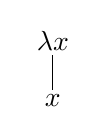
\begin{tikzpicture}[baseline=(root.base),level distance=5ex,inner ysep=0.5mm,sibling distance=10mm]
        \node (root) {$\lambda x$}child{node{$x$}};
    \end{tikzpicture}
    &
    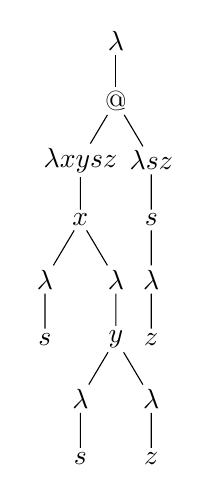
\begin{tikzpicture}[baseline=(root.base),level distance=5ex,inner ysep=0.5mm,sibling distance=9mm]
        \node (root)
        {$\lambda$}
        child {node{$@$}
            child{node{$\lambda x y s z$}
                child { node{$x$}
                    child{node{$\lambda$}{
                        child {node {$s$}}}
                    }
                    child{node{$\lambda$}
                        child{node{$y$}
                            child{node{$\lambda$}
                                child{ node {$s$}}
                            }
                            child{node{$\lambda$}
                                child{node{$z$}}}
                        }
                    }
                }
            }
            child{node{$\lambda s z$}
                child{node{$s$}
                    child{node{$\lambda$} child{node{$z$}}}
                }
            }
        };
    \end{tikzpicture}
    &
    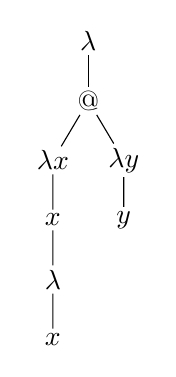
\begin{tikzpicture}[baseline=(root.base),level distance=5ex,inner ysep=0.5mm,sibling distance=9mm]
        \node (root)
        {$\lambda$}
        child {node{$@$}
            child{node{$\lambda x$}
                child { node{$x$}
                    child{node{$\lambda$}{
                        child {node {$x$}}}
                    }
                }
            }
            child{node{$\lambda y$} child{node{$y$}}}
        };
    \end{tikzpicture}
    &
    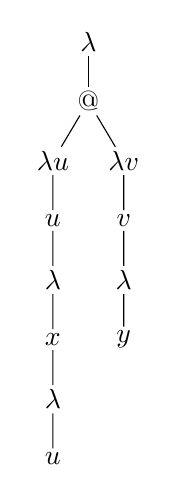
\begin{tikzpicture}[baseline=(root.north),level distance=5ex,inner ysep=0.5mm,sibling distance=9mm]
        \node (root)
        {$\lambda$}
        child {node{$@$}
                child{node{$\lambda u $}
                   child {node {$u$}
                      child {node {$\lambda$}
                          child {node {$x$}
                              child {node {$\lambda$}
                                  child {node {$u$}
                                  }
                              }
                          }
                      }
                   }
                }
                child{node{$\lambda v$}
                    child{node{$v$}
                        child{node{$\lambda$}
                            child{ node {$y$}}
                        }
                    }
                }
            };
        \end{tikzpicture}
    &
    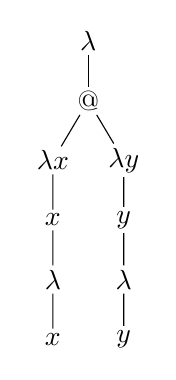
\begin{tikzpicture}[baseline=(root.base),level distance=5ex,inner ysep=0.5mm,sibling distance=9mm]
        \node (root)
        {$\lambda$}
        child {node{$@$}
            child{node{$\lambda x$}
                child { node{$x$}
                    child{node{$\lambda$}{
                        child {node {$x$}}}
                    }
                }
            }
            child{node{$\lambda y$}
                child { node{$y$}
                    child{node{$\lambda$}{
                        child {node {$y$}}}
                    }
                }
            }
        };
    \end{tikzpicture}
    \end{tabular}
\caption{Examples of trees of untyped lambda terms.}
\label{fig:comptree_examples}
\centering
\end{figure}

We define the \defname{enabling relation} $\enables$ on tree nodes $\Nodes$ as the relation mapping (i) each $\lambda$-node to all the variable nodes that it binds; (ii) the root of the tree to all the free variable nodes; (iii) variable and application node to each one of their child node.
We number children nodes starting from $0$ for @-nodes and from $1$ for variable nodes, so that the $0$th child denotes the operator of a redex, while other children represent operands of either an @-node or a variable node.
%
We write
$n \enables_k \lambda\overline{x}$, for $k\geq0$, to indicate that
lambda node $\lambda\overline{x}$ is the $k$th child of a variable or application node $n$;
$\lambda\overline{x} \enables_k n$, for $k\geq1$, to indicate that the label of a bound variable node $n$ is the $k$th variable name bound in $\lambda\overline{x}$, that is node $n$ is labelled $x_k$;
 and if $r$ denotes the root of the tree then we take the convention $r \enables_k z$ for any free variable node $z$, where $k$ denotes the free variable index of $z$ according to some predefined numbering of free variables.
%
We say that a node \defname{hereditarily enables} another node if the two nodes relate by the transitive closure of $\enables$.
%
A tree node is \defname{external} if it is hereditarily enabled by the root or it is the root itself, otherwise it is \defname{internal}. We write $\ExternalNodes$ for the set of external nodes.
We write $\InternalNodes$ to denote the set of internal nodes, which are therefore @-nodes and nodes hereditarily enabled by @-nodes.
The \defname{arity} of a node $n$, written $|n|$,
is defined for a variable node as the number of immediate arguments (\ie, children in the tree); for an application node, as the number of operands (\ie, number of children of the $@$-node minus 1); for a lambda node $\lambda x_1 \cdots x_k$, $k\geq 0$, as the number of bound variables $k$.

\subsection{Extensional tree}
We extend the notion of term tree by augmenting the
 \defname{structural nodes} $\Nodes$ of $\ctree(M)$, representing tokens in the syntax representation of the lambda term,
with two countable sets of \defname{ghost nodes} representing fictitious tokens: The \defname{ghost lambda nodes}  have a
 unique label $\ghostlmd$ and represent fictitious lambda abstractions.
The \defname{ghost variable nodes} have a unique label $\ghostvar$ and represent fictitious nameless variable nodes.
%; they are bound by either a structural lambda node from $\ctree(M)$ or by some ghost lambda node.
%
We define them by simultaneously and recursively
extending the parent-child node relation and the enabling relation
associated with the term tree: for every (ghost) variable or @-node $n$ with parent (ghost) lambda-node $\nu$, and for all $k>|n|$,
we introduce a new node $\ghostlmd$ as the $k$th-child of $n$,
and a new node $\ghostvar$ as the unique child of that ghost lambda node.
We extend the enabling relation with $n \enables_k \ghostlmd$
and $\nu \enables_{|\nu|+ k} \ghostvar$; where by convention ghost nodes have arity $0$, and the arity of structural nodes remains unchanged (\ie, given by their arity in the structural tree $\ctree(M)$).
%
This extended enabling relation induces a binding relation between ghost variables and their (possibly ghost) lambda-binder, which lets us forgo the notion of variables names in ghost nodes: we can thus
use respectively $\ghostlmd$ and $\ghostvar$ as a unique label for all ghost lambda and variable nodes.

The infinite tree hereby defined is called the \defname{extensional tree} $\exttree(M)$ over labels $\mathcal{L} \union \{ \ghostlmd, \ghostvar \}$.
Its nodes $\ExtendedNodes$ consists of structural nodes of $\Nodes$ plus all ghost variables $\ghostvar$ and lambda nodes $\ghostlmd$ as defined above.
We write $\ExtendedNodesLmd$ for the subset of lambda nodes (structural $\NodesLmd$ or ghosts $\ghostlmd$) and $\ExtendedNodesVar$ for variable nodes (structural $\NodesVar$ or ghosts $\ghostvar$).

\subsection{Justified sequence of nodes}
\label{sec:justseq}

A \defname{justified sequence} is defined a sequence of nodes in $\ExtendedNodes$ where every occurrence $n$ in the sequence may have an associated link called `justification pointer' pointing to some previous node occurrence $j$ in the sequence, called its `justifier', with an associated \defname{link label} $l\geq0$; with the constraint that the justifier node $\enables$-enables the source node with the corresponding label; that is $j \enables_l n$ must hold. The \defname{link distance} is the number of occurrences separating $n$ from its justifier $j$ plus $1$, or $0$ if $n$ has no justifier.
%
We represent a justified sequence as a sequence of labelled node occurrences with back-pointing arrows for justification pointers. For example: $\Pstr[10pt]{ \ldots (j){j} \ldots (n-j,25:l){n} }$, which we read `$n$ points to $j$', or `$n$ is justified by $j$' with link label $l$.
%
For readability, we sometimes indicate the link label in exponent of the justified occurrence instead of above the pointer, or we even omit the justification pointers altogether.
By abuse of notation, we often represent occurrences in justification sequences by their corresponding node labels so that for instance $\ldots \lambda\overline{x} \cdot x \ldots$ refers to an occurrence of a node in $\ExtendedNodesLmd$ labelled $\lambda\overline{x}$ followed by an occurrence of a node in $\NodesVar$ with label $x \in \VarSet$.
%
Note that the enabling relation is \emph{statically} induced by the term whereas the concept of justification is defined on node \emph{occurrences}, that is within a specific justified sequence. The \defname{set of justified sequences} over $M$, denoted $\justseqset(M)$, consists of all justified sequences over $\ExtendedNodes$.

Let $s$ denote a justified sequence. We write $s^\omega$ to denote the last occurrence of $s$. For any occurrence $n$ in $s$ we write $s_{\leq n}$ for the prefix of $s$ ending at $n$, and $s_{<n}$ for the prefix ending immediately before $n$.
%and $\jp(s)$ to denote the prefix of $s$ ending at the justifier of the last node of $s$.
We say that $s$ \defname{extends} $u$ if $u$ is a strict prefix of $s$.
A sequence $s$ is \defname{maximal} in $T\subseteq \justseqset(M)$ if there is no sequence in $T$ that extends it.
%
For any set $T\subseteq \justseqset(M)$ we write $T^{\max}$ for the subset of maximal sequences of $T$.
%
We borrow basic definitions from Game Semantics~\cite{Abr02}. A justified sequence verifies the \defname{alternation condition} if it starts with a lambda node and subsequently alternates between (i) a variable or application node (ii) a lambda node.
An occurrence in $s$ is \defname{hereditarily justified by some other occurrence} if recursively following justification pointers starting from the first occurrence leads to the second one.
Since justification pointers honor the enabling relation $\enables$, if an occurrence of node $n$ is hereditarily justified by the occurrence of a node $m\in\Nodes$ then $n$ is necessarily hereditarily enabled by $m$. Further, if $m$ occurs only once in $s$ then the occurrences hereditarily justified by $m$ are precisely the occurrences of nodes that are hereditarily \emph{enabled} by $m$ in $\ctree(M)$.
%
The \defname{projection} $s\filter n$ of $s$ with respect to $n$ is the subsequence consisting of occurrences hereditarily justified by $n$ in $s$. We write $s \filter A$ for the subsequence of $s$ consisting of occurrences of nodes in a subset $A \subseteq \Nodes$.
Hence $s\filter\ExternalNodes$ consists of occurrences of $s$ that are external nodes, or equivalently that are hereditarily justified by some occurrence of the root in $s$.

The P-view is the sub-sequence obtained by reading a justified sequence backwards and skipping occurrences lying under the justification pointer of a lambda node:

\begin{definition}
    \label{def:views}
\iflongversion %%%%%%%%%%
The \defname{P-view $\pview{s}$} of a justified sequence $s$ is defined recursively by:
$$\begin{array}{rcll}
 \pview{\epsilon} &=&  \epsilon \\
 \pview{s \cdot n }  &=&  \pview{s} \cdot n
    & \mbox{if $n$ is a variable or $@$ node;}
    \\
 \pview{\Pstr[10pt]{ s \cdot (m){m} \cdots (lmd-m,25){n}}} &=&
        \Pstr{ \pview{s} \cdot (m2){m} \, (lmd2-m2,30){n} }
    & \mbox{if $n$ is a lambda node;}
    \\
 \pview{s \cdot n }  &=&  n & \mbox{if $n$ is a lambda node with no pointer.}
\end{array}$$
%
The dual notion $\oview{s}$ of \defname{O-view} is given by
$\oview{\epsilon} = \epsilon$;
$\oview{s \cdot n }  =  \oview{s} \cdot n$ for $\lambda$-node $n$;
$\oview{\Pstr[10pt]{s \cdot (m){m} \cdots (x-m,30){x}}}= \Pstr{ \oview{s} \cdot (m2){m} \, (n2-m2,45){x} }$ for variable node $x$; and $\oview{s \cdot @ } = @$.
%
% Expanded version of the O-View definition:
% The dual notion of O-view, denoted $\oview{s}$, is defined by:
% $$\begin{array}{rcll}
%  \oview{\epsilon} &=&  \epsilon \\
%  \oview{s \cdot n }  &=&  \oview{s} \cdot n
%     & \mbox{if $n$ is an $\lambda$-node;}
%     \\
%  \oview{\Pstr[10pt]{s \cdot (m){m} \cdot \cdots \cdot (x-m,30){n}}} &=&
%     \Pstr{ \oview{s} \cdot (m2){m} \cdot (n2-m2,60){n} }
%     & \mbox{if $n$ is a variable node;}
%     \\
%  \oview{s \cdot n }  &=&  n
%     & \mbox{if $n$ is an $@$ node.}
% \end{array}$$
%
\else %%%%%%%%%% short
    The \defname{P-view $\pview{s}$} of a justified sequence $s$ is defined recursively by:
    $\pview{\epsilon} = \epsilon$,
    $\pview{s \cdot n } =  \pview{s} \cdot n$
        if $n$ is a variable or $@$ node;
    $\pview{\Pstr[10pt]{ s \cdot (m){m} \cdots (lmd-m,25){n}}} =
        \Pstr{ \pview{s} \cdot (m2){m} \, (lmd2-m2,30){n} }$
        if $n$ is a lambda node;
    and  $\pview{s \cdot n }  =  n$
        if $n$ is a lambda node with no pointer.
    %
    The dual notion $\oview{s}$ of \defname{O-view} is given by
    $\oview{\epsilon} = \epsilon$;
    $\oview{s \cdot n }  =  \oview{s} \cdot n$ for $\lambda$-node $n$;
    $\oview{\Pstr[10pt]{s \cdot (m){m} \cdots (x-m,30){x}}}= \Pstr{ \oview{s} \cdot (m2){m} \, (n2-m2,45){x} }$ for variable node $x$; and $\oview{s \cdot @ } = @$.
    %
    % Expanded version of the O-View definition:
    % The dual notion of O-view, denoted $\oview{s}$, is defined by:
    % $$\begin{array}{rcll}
    %  \oview{\epsilon} &=&  \epsilon \\
    %  \oview{s \cdot n }  &=&  \oview{s} \cdot n
    %     & \mbox{if $n$ is an $\lambda$-node;}
    %     \\
    %  \oview{\Pstr[10pt]{s \cdot (m){m} \cdot \cdots \cdot (x-m,30){n}}} &=&
    %     \Pstr{ \oview{s} \cdot (m2){m} \cdot (n2-m2,60){n} }
    %     & \mbox{if $n$ is a variable node;}
    %     \\
    %  \oview{s \cdot n }  &=&  n
    %     & \mbox{if $n$ is an $@$ node.}
    % \end{array}$$
    %
\fi
Given two occurrences $n$ and $m$ in a justified sequence $s$, we say that $n$ is \defname{visible at} $m$ just if $n$ occurs in the P-view $\pview{s_{\leq m}}$.
\end{definition}

%%%%%%%%%
\subsection{Name-free and name-preserving encoding}
The \defname{(name-free) structure} of a justified sequence is obtained by discarding node labels while preserving node types, arities and justification pointers. It is encoded as a sequence of elements from
$(\nat\times\nat\times\nat) +
   (\nat\times\nat)
   + \{ @ \}$
where $(a, j, i)$ represents a lambda occurrence of arity $a$
with link distance $j$ and link label $i$ ($0$ for no pointer);
$(j, i)$ represents a variable occurrence
with link distance $j$ and link label $i$;
and $@$ represents the occurrence of an application node.
%
Two sequences $s$ and $u$ over possibly two distinct terms are \defname{equivalent}, written $s \equiv u$ just if they have the same structure: the type (variable, @-node or $\lambda$-node), arity, link distance and link label of the underlying occurrences match pairwise. Two equivalent sequences are not necessarily equal since they may have different variable names.
Two subsets $J_1\subseteq \justseqset(M_1)$ and $J_2\subseteq\justseqset(M_2)$ are \defname{isomorphic}, written $J_1\structisomorphic J_2$, if  there exists a structure-preserving bijection between $J_1$ and $J_2$; that is a bijection $\phi :J_1\longrightarrow J_2$ such that $s\equiv\phi(s)$ for all $s\in J$.

\begin{example}
    Alpha-conversion preserves the structure so for instance we have
    $\Pstr[10pt]{ (l){\lambda x y} \, (n-l,25){x} } \equiv \Pstr[10pt]{ (l){\lambda z y} \, (n-l,25){z}}$.
\end{example}


The \defname{name-preserving encoding} of a justified sequence of nodes with variables in $\VarSet$ is a sequence of element in
$\nameencoding = (\mathcal{V}^*\times\nat\times\nat) +
   (\nat\times\nat)
   + \{ @ \}$  defined occurrence-wise similarly to the name-free encoding
 except for lambda nodes where
  an occurrence $\lambda\overline{x}\in\ExtendedNodesLmd$
 with link distance $j$ and link label $i$ gets encoded
 as $(\overline{x},j,i) \in \mathcal{E}$.
%
Replacing the second components of the lambda-nodes encoding by their length
yields the name-free encoding.
Reciprocally, given a fixed term, the list of variable names in each $\lambda$-occurrences is uniquely recoverable from the sequence structure and the enabling relation $\enables$ over $\exttree$.
%
%
%%%%% clashfree concatanation
% For any variables $\overline{x}\in\VarSet^*$
% and variable $y\in\VarSet$ we write $\overline{x} \otimes y$ for the list of variables obtained by appending $y$ to $\overline{x}$ without introducing any name clash: $\overline{x} \otimes y = \overline{x} \cdot y$ if $y\not\in\overline{x}$, and
% $\overline{x} \otimes y = \overline{x} \cdot y'$ if $y\in\overline{x}$ for some  variable $y'\in\mathcal{V}$ fresh in $\overline{x}$.
% For any $\overline{y} = y_1 \ldots y_m$, $m\geq 0$,
% we write $\overline{x} \otimes \overline{y}$ for $((\ldots(\overline{x} \otimes y_1) \otimes y_2) \ldots \otimes y_m)$.
%%%%%%
The \emph{readout function} $\readout: \nameencoding^* \rightarrow \mathcal{L}^*$
decodes a name-preserving encoding into a sequence of node labels in $\mathcal{L}$. It is defined by
$\readout[\epsilon]= \epsilon$;
$\readout[s \cdot @] = \readout[s] \cdot @$;
$\readout[s \cdot (\overline{x}, j, i) ] = \readout[s] \cdot \lambda\overline{x}$
and for any encoding $s = u \cdot (\overline{x}, k, l)\,  n_1 \ldots n_{j-1}$ where $u \in \nameencoding^*$, $n_1, \ldots n_{j-1}\in \nameencoding$, $j\geq 1$, $k,l\geq 0$,
$\readout[s\cdot (j,i)] = \readout[s] \cdot x_i$
if $i\leq |\overline{x}|$, and
$\readout[s\cdot (j,i)]  = \readout[s] \cdot \ghostvar$ if $i> |\overline{x}|$.
% $$
% \begin{array}{lll}
% \readout[u \cdot (\overline{x}, k, l)\,  n_1 \ldots n_{j-1}\, (j,i)]
% &=&
%  \begin{cases}
%    \readout[s] \cdot x_i &
%      \mbox{if $i\leq |\overline{x}|$.} \\
%    \readout[s] \cdot \ghostvar &
%      \mbox{if $i> |\overline{x}|$.}
% \end{cases}
% \end{array}$$
Just like the name-free encoding, this encoding assimilates the ghost lambda `$\ghostlmd$' with the dummy lambda `$\lambda$', so that the case $\lambda\overline{x}$ where $\overline{x}=\epsilon$ covers both the ghost lambda and dummy lambda.
%
We then define $\readout \colon \nameencoding^* \rightarrow \mathcal{L}^*$
by point-wise extension.

\begin{example}
\label{examp:ghost_materialization}
    Take the term $M = \lambda x. (\lambda y z.z) u$. The nodes of the extensional tree $\exttree(M)$ are $\ExtendedNodes = \{ \lambda x, @, \lambda y z, z, \lambda, u \} + \ghostvar + \ghostlmd$. The justified sequence
    $t = \Pstr[10pt]{
        (l){\lambda x} \, (a)@ \, (lyz-a,25:0){\lambda y z} \, (z-lyz,25:2)z \, (gl-a,35:2)\ghostlmd \, (gv-l,39:2)\ghostvar }
    $
    has name-preserving encoding
    $(x ,0,0)\cdot
    @\cdot
    (y\, z, 1,0)\cdot
    (1,2)\cdot
    (\epsilon,3,2)\cdot
    (5,2)$, whereas
    the sequence encoding
    $ (x\, g, 0, 0)\cdot
    @\cdot
    (y\, z\, x\, y\, y, 1,0)\cdot
    (1,2)\cdot
    (\epsilon,3,2) \cdot
    (5,2)$ encodes the justified sequence
    $s= \Pstr[10pt]{
        (l){\lambda x g}
         (a)@
         (lyz-a,25:0){\lambda y z x y y}
         \,(z-lyz,30:2)z
         (gl-a,35:2)\ghostlmd
         (gv-l,40:2)\ghostvar }
    $ which reads out as $\readout[s]= \lambda x g \cdot @ \cdot \lambda y z x y y \cdot z \cdot \lambda \cdot g$.
\end{example}

%%%%%%%%%%%%%%%%% end of `name-preserving' presentation

The main results of the paper apply to both encodings, though
the name-preserving presentation has the advantage of reusing names from the original terms when producing the normal form.
We thus adopt that encoding in the rest of the paper and take $\justseqset(M)$ to be a (strict) subset of $\nameencoding^*$.

\subsection{Justified paths of the term tree}

We define the \defname{set of justified paths} $\pathset(M)$ of a term $M$ as the set of justified sequences in $\justseqset(M)$
whose underlying sequences of nodes are those from the paths of the labelled-tree $\ctree(M)$ and justification pointers are induced by the enabling relation:
 %
 bound variable nodes point to their binder $\lambda$-node, which necessarily occurs in the path to the root, with link label set to the index of the variable name in the binding $\lambda$-node;
 %
 free variables point to the initial occurrence (the tree root) with link label  set to an index in $\nat$ uniquely identifying the
 free variable name;
 %
 and lambda nodes are justified by the immediate predecessor in the path sequence, which is also its parent node by definition of a tree path, with label index given by its child index.
 %
\begin{property}[Path Characterization]
\label{prop:tree_path_charact}
 An untyped term $M$ is uniquely determined
(i) by the maximal justified paths of $\pathset(M)$;
or (ii) up to $\alpha$-conversion, by the \emph{structure} of the maximal justified paths of $\pathset(M)$.
\end{property}
\begin{proof}
(i) A $\lambda$-term $M$ is uniquely determined by its term tree $\ctree(M)$, itself uniquely determined by its maximal paths, which can be reconstructed from the justified maximal paths (labels are the same, and the child index is $1$ for variable/@ nodes and is given by the justification label for lambda nodes).
%
(ii) Variables bindings are uniquely determined by the justification pointers with their associated label; so maximal justified paths are  reconstructible from their structure, up to $\alpha$-conversion, by assigning fresh variable names to all lambda-nodes.
\end{proof}

\begin{example}
    The maximal justified paths of
  $\pathset((\lambda x.x y) (\lambda z.z))$
  are
  $\{
  \Pstr{ (r){\lambda} (at){@} (lx-at,30:0){\lambda x} (x-lx,30:1){x} (l2-x,30:1){\lambda} (y-r,40:1){y} },
  \Pstr{ (r){\lambda} (at){@} (lz-at,35:1){\lambda z} (z-lz,35:1){z}}
  \}$.
\end{example}

%%%
A set of name-preserving justified sequences $T\subset \nameencoding^*$ is \defname{$\alpha$-consistent} if all its path-like justified sequences agree on how to name variables in lambda nodes: if $p \cdot (\overline{x}, 1, i)$ and $p \cdot (\overline{y}, 1, i)$ are in $T$ for $i\geq 0$, $p\in \nameencoding^*$ then $\overline{x} = \overline{y}$.

\begin{proposition}[Name-preserving term read-out]
\label{proposition:termtree_readout_from_justitied_paths}

Let $T\subset \nameencoding^*$ be a finite set of (name-preserving encoded) justified sequences  that is $\alpha$-consistent.
If $T\structisomorphic \pathset(M)$ for some (a priori unknown) untyped term $M$ then one can effectively read out from $T$ an untyped
term  $\readout[T]$ that is $\alpha$-equivalent to $M$.
%
Furthermore, provided that no variable capture situation occurs, the variable  occurring in $\readout[T]$ preserves original names from lambda-occurrences in $T$.
\end{proposition}
%(Then $T$ is path-like, that is lambda-nodes are justified by their immediate predecessor in the sequence.)
\begin{proof}
    Because $T \structisomorphic \pathset(M)$, the sequences in $T$ have the properties
of justified paths of a term tree: they start with a lambda, alternate between lambda and variable/@, lambdas have
a single child, and are necessarily justified by their immediate predecessor in the sequence (their parent).
Furthermore, $T$ induces an arity for each occurrence of a sequence in $T$: the arity of a lambda-occurrence $(\overline{x},j,i)\in\nameencoding$ is $|\overline{x}|$, the arity of a variable or @-occurrence is the maximum
child-index (given by the link label) of any lambda occurrence immediately following it in any sequence of $T$.

This allows us to construct a $\mathcal{L}$-labelled tree
inductively from the maximal sequences of $T$.
We first inductively construct a $\mathcal{L^-}$-labelled tree with
$\mathcal{L^-} = \{ @ \} + \{
    \lambda \overline{x} \ | \
    \overline{x} \in \mathcal{V}^* \} + \nat\times\nat$,
where a De Bruijn pair $(j,i)\in \nat\times\nat$ represents a variable node such that the link distance $j$ identifies the binder lambda-node, and the link label $i$ gives the bound variable index in that binding lambda node. Since $T$ is $\alpha$-consistent, there is a single choice of variable names $\overline{x}$ to assign to a given lambda-node.

An important step at this point is to rename variables to avoid any potential variable capture when we finally replace the De Bruijn pairs by the variable names they refer to.
%
Firstly, the variable names $\overline{x}$ from lambda-occurrences in sequences in $T$ may contain duplicates. We resolve this by renaming names that are repeated within the same lambda node, provided that some variable occurrence under that node refers to the first variable name: this is the situation of a justified path  $\cdots \lambda x x y \cdots (j,1)$ where the De Bruijn pair $(j,1)$ refers to the first $x$ of the lambda node. In this case, the lambda node becomes $\lambda x x' y$.
%
Secondly, two distinct nested lambdas in a given justified path may bind the same variable name. If this introduces a clash, \ie, the variable occurs freely under the nested lambda, then we rename the bound variable in the nested lambda. This is the situation of a justified path of the form $\cdots \lambda{xyz} \cdots \lambda {xuv} \cdots (j,1) \cdots$
 where the De Bruijn pair $(j,1)$ refers to the $x$ from the first lambda $\lambda{x y z}$.

After renaming variables in the $\mathcal{L^-}$-labelled tree, we obtain the final $\mathcal{L}$-labelled tree by replacing all De Bruijn pairs $(j,i)$ with the $i$th variable name from the lambda node located $j$ nodes above it in the term tree, as implemented by the name-preserving readout function $\readout[\_]$ on justified sequences.
%
Interpreting that $\mathcal{L}$-labelled as a term tree $\ctree(\_ )$ lets us read back from it the underlying untyped term $N$.
%
By construction we have $\pathset(N) = T$ therefore
$N$ and $M$ have the same justified paths structures so by
Property~\ref{prop:tree_path_charact} they must be $\alpha$-equivalent.
\end{proof}


\section{Imaginary Traversals}
\label{sec:imaginary_traversals}
\subsection{Definition and properties}

\begin{definition}
The set $\travulc(M)$ of \defname{traversals} of an untyped lambda term $M$, abbreviated $\travulc$ when the term is clear from context, is the set of justified sequences of nodes over the extensional tree of $M$, defined inductively by the derivation rules of Table~\ref{tab:trav_rules}:
 $t \in \travulc(M)$ if and only if the judgment $\istraversal t$
 is derivable.
%
 We use interchangeably `\emph{imaginary traversal}' or just `\emph{traversal}' when referring to a traversal of an untyped term.
\end{definition}

\begin{table}[!t]
\begin{ruletablebox}{} %{Imaginary traversals of $\lambda$-calculus}
\noindent {\bf PROGRAM -- Structural rules}
\begin{itemize}[leftmargin=3em]
    \item[\rulenamet{Root}]
    $\istraversal \nu$ if $\nu$ is the root $\lambda$-node of the term tree $\ctree(M)$.

    \item[\rulenamet{App}] If $\istraversal t \cdot @$ then
    $\istraversal \Pstr[0.4cm]{t \cdot (at) @  \, (a-at,40:0) \nu}$ where $\nu\in\NodesLmd$ is the $0$th child $\lambda$-node of $@$.

    \item[\rulenamet{Lam}] If $\istraversal t \cdot \nu$ for $\nu\in\ExtendedNodesLmd$ then $\istraversal t \cdot \nu ~ n$ where $n$ is $\nu$'s unique child and if $n$ is
    \begin{compactitem}
        \item[\rulenamet{Lam^@}] an $@$-node then it has no justifier;
        \item[\rulenamet{Lam^{\sf var}}] in $\NodesVar$ then it points to the only occurrence in $\pview{t\cdot \nu}$ of a node $m$ verifying $m \enables_k n$ for some $k\geq 0$, and has link label $k$;

        \item[\rulenamet{Lam^\ghostvar}] a ghost variable $\ghostvar$
        (thus $\nu$ is $\ghostlmd$) then
        it points to the predecessor $\mu$ of $\nu$'s justifier $m$, and has link label $|\mu| + i - |m|$
        where $i$ is the link label of $\nu$. That is
        $\istraversal \Pstr[0.5cm]{ u \cdot(alphaprime){\mu}\, (m){m} \cdot v \cdot  (gl-m,30:i){\ghostlmd}\, (al-alphaprime,43:{|\mu| + i - |m|}){\ghostvar}}$
    where
        $t \cdot \nu = \Pstr[0.5cm]{ u \cdot
        \mu \, (m){m} \cdot v \cdot (gl-m,40:i){\ghostlmd}}$,
        $\mu  \in \ExtendedNodesLmd, m \in\ExtendedNodesVar \union \NodesApp$.
    \end{compactitem}
\end{itemize}
\emph{\bf PROGRAM -- Copy-cat rule}
\begin{itemize}[leftmargin=3em]
\item[\rulenamet{Var}] If $\istraversal \Pstr[0.5cm]{t\cdot(m){m}
 \, (alphaprime){\mu}
\cdot v \cdot (n-alphaprime,50:i){n}}$ for $m \in\ExtendedNodesVar \union \NodesApp$, $\mu \in \ExtendedNodesLmd\inter\InternalNodes$, $n \in \ExtendedNodesVar\inter\InternalNodes$, $i>0$ then
  $\istraversal \Pstr[0.3cm]{ t  \cdot
(m){m}\, (lx){\mu}  \cdot v \cdot (x-lx,30:i){n}
    \, (letai-m,45:i){\nu}}$
    where $\nu$ denotes the $i$th child ($\lambda$-node) of $m$.
\end{itemize}

\emph{\bf DATA -- Input-variable rule}
\begin{itemize}[leftmargin=3em]
\item[\rulenamet{IVar}] If $\istraversal t \cdot n$ with $n \in \ExtendedNodesVar \inter \ExternalNodes$ then
for every $i$th child $\nu$ of any node $m \in \ExtendedNodesVar$ occurring in $\oview{t\cdot n}$, $i\geq1$, we have
$\istraversal t \cdot n ~ \nu$ where $\nu$ points to $m$ with label $i$.
\end{itemize}

where $u,v$ denote sub-sequences of justified sequences of nodes.
\caption{Derivation rules of imaginary traversals $\travulc$ of the untyped $\lambda$-calculus.}
 \label{tab:trav_rules}
\end{ruletablebox}
\end{table}

\begin{example}
\label{ex:ulctrav_sample}
Take the term $J = (\lambda u . u(x\,u)) (\lambda v . v\,y)$, whose tree is represented in Figure~\ref{fig:comptree_examples}. We have the traversal
$t = \Pstr[0.7cm][1pt]{(n0){\lambda}
(n1){@}
(n2-n1){\lambda u^0}
(n3-n2){u^1}
(n4-n1){\lambda v^1}
(n5-n4){v^1}
(n6-n3){\lambda^1 }
(n7-n0){x^1}
(n8-n7){\lambda^1}
(n9-n2){u^1}
(n10-n1){\lambda v^1}
(n11-n10){v^1}
(n12-n9){{\ghostlmd^1}}
(n13-n8){{\ghostvar^1}}
(n14-n13){{\ghostlmd^1}}
(n15-n12){{\ghostvar^1}}
(n16-n11){\lambda^1 }
(n17-n0,30){y^2}} \in \travset(J)$
where each justification label is indicated in exponent of the corresponding justified occurrence.
\end{example}

\begin{proposition}
\label{prop:ulctrav_welldefined_pathview}
The traversal rules are well-defined, in particular for any sequence of nodes with pointers $t\in \travset$ we have:
\begin{compactitem}
\item[(i)] $t$ is a valid justified sequence, with respect to
the enabling relation $\enables$ on $\ExtendedNodes$, and verifies the alternation condition;
%(ii) and if the last node in $t$ is external then so are all the nodes in $\oview{t}$. % By induction on \oview{t}
\item[(ii)] For all occurrences $\Pstr[0.5cm]{(m){m} \cdots (n-m,30:i){n}}$, $n$ is a ghost node if and only if $i > |m|$;
\item[(iii)] $\pview{t}$ is a (justified) path in the extensional tree $\exttree(M)$;
So if $t$ does not contain ghost nodes then $\pview{t}$ is a structural path in $\ctree(M)$.
\end{compactitem}
\end{proposition}
\shortproof
Proven simultaneously by induction on the traversal rules.
For \rulenamet{Lam^{\sf var}}: By induction hypothesis (iii) the P-view is a path in the extensional tree of $M$. But the last node of $t$ is a structural node therefore, this path is necessarily a structural path with no ghost node. Consequently, if the last node is a bound variable node, its enabler is precisely its binding lambda node which necessarily occurs exactly once in the path to the root. If the variable is free then the enabler is the root itself and (i) holds. By definition, the justification pointer honors the enabling relation so (ii) holds. The node $n$ is by definition the unique child of $\nu$ thus (iii) holds.
%
For \rulenamet{Lam^\ghostvar}, the induction hypothesis (ii) shows that $i>|m|$, which guarantees that $|\mu|+i-|m|>0$ is a valid justification label (i) and that (ii) holds for the traversed ghost node $\ghostvar$.
Finally (iii) holds because the node preceding $\ghostvar$ in the P-view is precisely $\mu$, its parent node.
%
Other rules are straightforward.
\endshortproof

The last property generalizes a concept from the theory of traversals~\cite{OngLics2006,BlumPhd} to the untyped setting: The game-semantic concept of P-views corresponds to paths in the computation tree.
% For any $t\in \travset$, the sequences $t\filter\ExternalNodes$ is a valid justified sequences verifying the alternation condition.


\paragraph{On-the-fly eta-expansion}
The rules \rulenamet{Var} and \rulenamet{IVar} are responsible for
performing the `on-the-fly expansion'.
If the arity of the traversed variable is sufficiently high, the tree statically dictates the structural node to traverse next: we have $i \leq |m|$ and $\nu$ is a structural lambda node in $\NodesLmd$; we call this the \defname{concrete sub-case}. Otherwise, the variable arity is too low to statically determine the requested operand of the application: $i > |m|$ and $\nu$ is a ghost lambda node $\ghostlmd$; we call this the \defname{imaginary sub-case}.

\begin{definition}
    \defname{Ghost materialization} refers to the instantiation of a traversal rule where the last occurrence prior to applying the rule is a ghost
    and the node traversed is structural.
    %%%%%% remark 1: materialization
    %
    Inspection of the traversal rules shows that this may only happen in rule \rulenamet{Var}, so that once a traversal starts traversing ghost nodes, the only way to `return' to structural nodes is via \rulenamet{Var} with a traversal of the form
    $
    \Pstr[0.5cm]{ t \cdot (y){y} \, (l){\nu}  \cdots (t-l,30:i){\ghostvar}
        \, (lx-y,40:i){\lambda \overline{x}}}
    $
    where
     $\lambda \overline{x} \in \NodesLmd$ is the $i$th child lambda node of some structural variable node $y \in \NodesVar$,
     and $\nu$ is a $\lambda$-node verifying $0\leq |\nu| < i \leq |y|$.
    %%%%%%%%
\end{definition}

Rule \rulenamet{Lam} traverses a lambda node by just visiting its unique child  in the tree, which is necessarily a structural node. Its counterpart \rulenamet{Lam^\ghostvar} traverses a ghost lambda by visiting the imaginary ghost variable that would be created if we were to eta-expand the sub-term under that lambda: the ghost placeholder $\ghostvar$ represents an occurrence of the $j$th variable bound by lambda node $\mu$ if the sub-term at node $\mu$ were eta-expanded $i-|n|$ times; hence $j = |\mu| + i - |m|$.
Observe that we necessarily have $i>|n|$ since the $i$th child of $n$ is a ghost variable node.

The successive fictitious eta-expansions of $M$ can be reconstructed from the traversal itself:
\begin{definition}
\label{def:onthefly_etaexpansion}
Let $M$ be an untyped term and $n\in \Nodes$ be the root node of some subterm $N$. We define ${\sf ETA}(M, n, k)$ as $M$
if $k \leq 0$ ; and for $k> 0$ as the term obtained from $M$ by substituting in-place $N$ with $\lambda z_1 \cdots z_k. N z_1 \cdots z_k$ for some variables $z_1, \ldots, z_k$ fresh in $N$.
%
We define inductively $M^t$,  the \defname{eta-expansion of $M$ with respect to a finite traversal $t$}, by $M^\epsilon = M$,
$M^{u \cdot n} = M$ if $n$ has no justifier, and if $m$ denotes $n$'s justifier in $u$ with link label $i$ then $M^{u \cdot n} = {\sf ETA}(M^{u}, m, i-|m|)$.
%
(Note that $i>|m|$ holds only for the imaginary sub-case of \rulenamet{Var} and \rulenamet{IVar}.)
\end{definition}

\iflongversion
It follows that $M$ is a sub-tree of $M^t$: paths in $\ctree(M)$ are also paths in $\ctree(M^t)$.
\fi

\begin{example}
The eta-expansion of $J = (\lambda u . u(x\,u)) (\lambda v . v\,y)$ with respect to traversal $t$ from Example~\ref{ex:ulctrav_sample} is
$J^t = (\lambda u . u(x (\lambda z_1. u (\lambda z_2.z_1\,z_2))) (\lambda v . v\,y)$
for some fresh variable names $z_1, z_2$.
\end{example}


\begin{proposition}
\label{prop:eta_expanded_trav}
Let $M$ be an untyped term and $t$ be a \emph{finite} traversal of $M$.
There exists a one-to-one function $\eta_t : \ExtendedNodes(M) \longrightarrow \ExtendedNodes(M^t)$
such that its implicit \emph{element-wise pointer-preserving} extension $\eta_t : \mathcal{J}(M) \longrightarrow \mathcal{J}(M^t)$ verifies the properties:
\begin{enumerate}[label=(\roman*),nosep]
    \item If $u \in \travulc(M)$ then $\eta_t(u) \in \travulc(M^t)$,
    and thus $\pview{\eta_t(u)}$ is a \emph{structural} path in $\ctree(M^t)$.

    \item If $v \in\travulc(M^t)$ then there exists
    a traversal $u\in\travulc(M)$
    %(with possibly ghost nodes)
    such that $v = \eta_t(u)$.

    \item The restriction of $\eta_t$ to $\travset(M)$ defines a structure-preserving bijection with $\travset(M^t)$.
\end{enumerate}
\end{proposition}
\shortproof
The tree $\ctree(M)$ being by definition a subtree of $\ctree(M^t)$, induces a one-to-one mapping $\eta_t$ from $\Nodes(M)$ to $\Nodes(M^t)$ which we extend point-wise to justified sequences. We show (i) by induction on $u$ observing that in the imaginary sub-case, the rules \rulenamet{Var} and \rulenamet{IVar} increase the arity of the justifier node $m$, which guarantees that the corresponding structural node exists in $\ctree(M^t)$. (ii) is shown similarly by induction on $v$.
(iii) follows from (i) and (ii).
\endshortproof
\proofatend
The tree $\ctree(M)$ being by definition a subtree of $\ctree(M^t)$, induces a one-to-one mapping from $\Nodes(M)$ to $\Nodes(M^t)$.
We extend it to ghost nodes by mapping ghost occurrences in $t$ to the corresponding node resulting from the eta-expansions of subterms of $M$ in $M^t$, and all other ghost nodes not occurring in $t$ to the corresponding ghost nodes in $\ctree(M^t)$. Formally, we define $\eta_t$ by induction on the traversal $t$, observing that the eta-expansion performed in rules \rulenamet{Var} and \rulenamet{IVar} in Definition~\ref{def:onthefly_etaexpansion} increases the arity of the justifier node $m$, which guarantees that the corresponding structural node exists in $\ctree(M^t)$.

(i) By induction on $u$. Reusing the rule used to traverse $u$ to traverse $\eta_t(u)$. For \rulenamet{Var} and \rulenamet{IVar}, in the \emph{imaginary} sub-case, if the ghost variable traversed also appears in $t$ then we use instead the \emph{concrete} sub-case of the corresponding rule to traverse $\eta_t(u)$.

(ii) By induction on $v$, applying to $u$ each rule that is applied to $v$. For the case \rulenamet{Var} and \rulenamet{IVar}, if the index $i$ is greater than the arity of the node $m$ in $M$ then the lambda node from $v$ gets replaced by a ghost lambda node in $u$.

(iii) By (i) the function is well-defined, it is injective by definition, and by (ii) it is surjective.
\endproofatend

\begin{example}
Continuing with Example~\ref{ex:ulctrav_sample},
the traversal $t$ of $\ctree(J)$ corresponds to the
traversal
$\Pstr[0.7cm]{
 (n0){\lambda}
 \, (n1){@}
 \, (n2-n1){\lambda u}
 \, (n3-n2){u}
 \, (n4-n1){\lambda v}
 \, (n5-n4){v}
 \, (n6-n3){\lambda}
 \, (n7-n0){x}
 \, (n8-n7){\lambda z_1}
 \, (n9-n2){u}
 \, (n10-n1){\lambda v}
 \, (n11-n10){v}
 \, (n12-n9){\underline{\lambda z_2}}
 \, (n13-n8){\underline{z_1}}
 \, (n14-n13){\underline{\lambda}}
 \, (n15-n12){\underline{z_2}}
 \, (n16-n11){\lambda}
 \, (n17-n0,30){y} }$
 of $\ctree(J^t)$.
\end{example}


\paragraph{Strands of traversals}

\begin{definition}
    \label{ref:strand}
    A \defname{strand} of a traversal, is a sub-sequence of consecutive occurrences of even length, starting with an external lambda node and ending with an external variable node, with only internal node occurrences in-between.

    From the parity property of traversals, a strand must consist of alternations of lambda nodes and variable/application nodes. To highlight a strand within a traversal we sometimes underline its opening and closing occurrence as follows:
     $ t = \cdots \underline{\nu_k}\ n_k\ \nu_{k-1}\ n_{k-1}\ \cdots\ \nu_2\ n_2\ \nu_1\ \underline{n_1} \cdots $
for some $k\geq 1$ where for $1 \leq j \leq k$, $\nu_j$ is in $\ExtendedNodesLmd$, $n_j$ is in $\ExtendedNodesVar\union\NodesApp$,
the external lambda $\nu_k$ and external variable $n_1$ delimit the strand boundaries and the $2k-2$ nodes in-between are all internal.
\end{definition}

A traversal has \defname{complete strands}
if each strand initiated by an external lambda occurrence
eventually ends with an occurrence of an external variable.
Otherwise, we say that the last strand in the traversal is \emph{incomplete}.
%
A finite \emph{maximal} traversal has necessarily complete strands, for if it were not ending with an external variable we could extend it with either \rulenamet{App}, \rulenamet{Lmd} or \rulenamet{Var}.
%

\paragraph{Traversal core}

In the typed setting, the \emph{core of a traversal}~\cite{BlumPhd} is simply obtained by removing all internal occurrences from a traversal.
Generalizing this notion to the untyped setting requires
additional relabelling of lambda nodes.

We consider sequences in $\VarSet^*$ as stacks of variable names equipped with  push and pop operations: for any stack $\overline{x} = x_1 \ldots x_n$, $n,j\geq0$, $pop_j (x_1 \ldots x_n) = x_{j+1} \ldots x_n$ if $j<n$, and $pop_j (x_1 \ldots x_n) = \epsilon$ otherwise;
pushing elements onto the stack is done via sequence concatenation:
 pushing  variable names $\overline{x}$, read from right to left, onto stack $\overline{y}$ yields  $\overline{x} \cdot \overline{y}$.

\begin{definition}[Core projection]
\label{def:coreprojection}
Let $\overline{y} \in \VarSet^*$ denote a stack of variable names.
We define the partial function $\coresymbol_{\overline{y}}\colon \justseqset(M) \longrightarrow \justseqset(M)$ on finite justified sequences by induction: $\coresymbol_{\overline{y}}(\epsilon) = \epsilon$, and for any justified sequence $s \cdot n\in\justseqset(M)$ with prefix $s \in \justseqset(M)$ and node occurrence $n\in\ExtendedNodes$:
\begin{equation*}
\coresymbol_{\overline{y}}(s\cdot n) =
\begin{cases}
%%%%
    \coresymbol_{\epsilon}(s) \cdot n
    & \mbox{if } n\in\ExtendedNodesVar\inter\ExternalNodes, \\
     \coresymbol_{pop_{|n|}(\overline{y})}(s)
    & \mbox{if } n\in(\ExtendedNodesVar\inter\InternalNodes)\union\NodesApp, \\
    \coresymbol_{\epsilon}(s) \cdot \lambda \overline{z}
    & \mbox{if $n  \in\ExtendedNodesLmd\inter\ExternalNodes$,
     $n$ is labelled $\lambda\overline{x}$ and $\overline{z}=\overline{x}\cdot\overline{y}$} \\
    \coresymbol_{\overline{x} \cdot \overline{y}}(s)
    & \mbox{if $n \in\ExtendedNodesLmd\inter\InternalNodes$
         and $n$ is labelled $\lambda\overline{x}$.}
%%%% Uncomment if want to make ghost lambda case explicit
% \coresymbol_{\epsilon}(s) \cdot\lambda\overline{y}
%     & \mbox{if } n\in\ghostlmd\inter\ExternalNodes, \\
% \coresymbol_{\overline{y}}(s)
%     & \mbox{if } n\in\ghostlmd\inter\InternalNodes.
%%%%%
\end{cases}
\end{equation*}
where the original justification pointers are preserved (that is the link distance of each occurrence is adjusted for the occurrences removed between it and its justifier). This is well-defined since an external node can only be justified by another external node. (Note that the last two equalities handle the ghost lambda case when $\overline{x}=\epsilon$.)
We call $\core{s} = \coresymbol_\epsilon(s)$ the \defname{core} of $s$,
and $\pview{\core{s}}$ its \defname{core P-view}, the P-view of its core.
\end{definition}

The subscript parameter in `$\coresymbol_{\overline{y}}$' is called \defname{stack of pending lambdas}. As $\coresymbol$ reads a strand backwards, it accumulates variable names which then get discharged onto the opening lambda node of the strand.
\iflongversion
So in words, the \emph{core projection} is the sub-sequence obtained by removing all internal nodes and discharging on each external lambda node the stack of \emph{pending lambdas} at that point.
\fi
This definition has a name-free counterpart that uses a stack length argument in place of the stack argument $\overline{y}$.
%
To aid with the calculation of the traversal core we will sometimes indicate the pending lambdas in exponent of external lambda nodes as follows:
$\cdots  \lambda\overline{x}^{[\overline{y}]} \cdots$ where $\overline{y}$ denotes the pending lambdas at $\lambda\overline{x}$.

Some immediate properties follow:
(i) The core of a justified sequence only contains external nodes therefore $\coresymbol$ is idempotent.
(ii) If $M$ is in beta-normal form then all the nodes of
 $\exttree(M)$ are external, so that the core projection coincides with the identity.
(iii) When discharging new variable names onto a lambda node, core projection can cause variable name reuse, but the justification pointers from the underlying name-free structure prevent any possible ambiguity.

\begin{example}The traversal $t = \lambda w^{[y]} ~ @ ~ \lambda x y ~ x ~ \lambda ~ z$ of $\lambda w . (\lambda x y .x) z$
    has core $\coresymbol(t) = \lambda w y ~ z$.
\end{example}


\begin{example} Take $(\lambda x. x x)(\lambda y. y)$ with traversal
$t$ represented below. Projecting nodes hereditarily justified by the root gives
$t\filter \ExternalNodes =  \Pstr[0.7cm]{(n0){\lambda^{[y]}}\ (n1-n0){{\ghostvar^1}}}$
while the core projection gives
$\coresymbol(t) = \Pstr[0.7cm]{(n0){\lambda y}\ (n1-n0){y}}$.
$$t = \Pstr[0.5cm]{
    (n0){\lambda}
    \,(n1){@}
    \,(n2-n1){\lambda x}
    \,(n3-n2){x}
    \,(n4-n1){\lambda y}
    \,(n5-n4){y}
    \,(n6-n3){\lambda }
    \,(n7-n2){x}
    \,(n8-n1){\lambda y}
    \,(n9-n8){y}
    \,(n10-n7){\ghostlmd^{1}}
    \,(n11-n6){\ghostvar^{1}}
    \,(n12-n5){\ghostlmd^{1}}
    \,(n13-n4){\ghostvar^{2}}
    \,(n14-n3){\ghostlmd^{2}}
    \,(n15-n2){\ghostvar^{2}}
    \,(n16-n1){\ghostlmd^{2}}
    \,(n17-n0){\ghostvar^{1}}
}$$
\end{example}



\subsection{Eta-long traversals of simply-typed terms}
Traversals for simply-typed languages, such as STLC and PCF, were previously studied in~\cite{BlumPhd}.
A notable limitation is that the tree traversed is built from the
 \defname{eta-long form} of the term, a conversion that involves eta-expanding some subterms so as to ensure that every strict subterm that is not of atomic type has necessarily another term applied to it. We omit the formal definition~\cite{huet75-unification, BlumPhd, OngLics2006} which is not essential.
 Effectively, this means that the tree is obtained by eta-expanding all variable and application nodes according to the type of the corresponding subterm: if it is $\tau_1 \rightarrow \ldots (\tau_m \rightarrow o)$ and the node has $n$ children with $n< m$ then the subterm is eta-expanded $m-n$ times.
Variable names in the lambda nodes labels are \emph{typed-annotated}, but those annotations are not used in any way by the  traversals rules. We can thus apply the rules of Table~\ref{tab:trav_rules} on a typed-term by just erasing all its types.
With this assumption, the definition of traversals from the typed settings \cite{BlumPhd} coincides with the following definition.
We consider a typed-term $M^\tau$ of simple type $\tau$ and without loss of generality, and to simplify notations, we assume that it is closed (no free variable).

\begin{definition}
\label{def:concrete_traversals}
A \defname{concrete traversal} is an imaginary traversal that does not contain
any ghost occurrence.
%
The set $\travset_\concrete$ of \defname{concrete traversals}
is defined by the rules of Table~\ref{tab:trav_rules}
with the exclusion of \rulenamet{Lam^\ghostvar} and by restricting rules \rulenamet{Var} and \rulenamet{IVar} to their concrete sub-case where the traversed node must be structural (\ie, $i\leq|m|$).
\end{definition}

\begin{definition}[Reformulation of~\cite{BlumPhd}]
The \defname{eta-long traversals} of a simply-typed term $M^\tau$ with eta-long form $N^\tau$ are defined as $\travset_{\concrete}(N^\tau)$, the concrete traversals of its eta-long form.
\end{definition}

\begin{proposition}
\label{prop:ulc_and_stlc_trav_coincide}
The eta-long traversals of an eta-long term $M^\tau$ are also obtained from
$M^\tau$ by restricting only the imaginary traversal rule \rulenamet{IVar} to its concrete sub-case.
\end{proposition}
\begin{proof}
Because the term is eta-long, the condition $i>|m|$ in rule \rulenamet{Var} never holds while traversing the term. This is shown by induction on the rules, observing that the arity of an $@$-node is necessarily equal to the arity of its $0$th child lambda node, and the arity of a variable node with binding index $i$ is necessarily equal to the arity of the $i$th child of its binder's parent.
Since we explicitly exclude the imaginary sub-case of \rulenamet{IVar}, the rules match with those of $\travset_\concrete$.
\end{proof}


\section{Evaluation with Traversals}
\label{sec:normalizing_trav}

The idea of evaluating lambda terms with traversals stems from the \emph{Normalized Paths Characterization} which states that the set of P-views of traversal cores captures what is strictly required from traversals to reconstruct the normal form of a term when it exists.
This was previously shown for simply-typed terms in eta-long form via
correspondence with Game Semantics.
We recall this result
in Proposition~\ref{prop:path_charact_stlc},
and prove its untyped counterpart in
Section~\ref{sec:correctness_ulc_normalization} using instead a term-rewriting argument (Theorem~\ref{thm:path_charact_ulc}).
This characterization suggests a normalization method by simply enumerating all the maximal traversals.
The challenge is to deal with arbitrarily long traversals as well as the infinite number of finite traversals (even for terms with a normal form!),
two situations caused by the generous non-determinism of rule \rulenamet{IVar}.
%
Fortunately, not all traversals are needed: a traversal shall be considered redundant if there exists a shorter one with identical core P-view.
In other words, we just need a subset covering
every possible core P-view.
%
We first consider the subset of \emph{essential traversals} which
meets this requirement.
Since its concrete subset is finitely enumerable, it gives
a normalization procedure for eta-long simply-typed terms.
To address the general untyped case,
we introduce \emph{normalizing traversals}, a larger subset
with a more relaxed non-determinism in \rulenamet{IVar} than the concrete restriction.

\subsection{Essential traversals}

Imaginary traversals may be infinitely long.
This is expected for non-normalizing terms such as $\Omega = (\lambda x. x x)(\lambda y. y y)$ which has the infinite traversal $\lambda x \cdot x \cdot \lambda y \cdot y \cdot x \cdot \lambda y \cdot y \cdot \ldots$ But this also occurs for terms with a normal form. Take for example $M = \lambda f . f (\lambda x. x)$, then for all $k\geq0$ the justified sequence $t_k = \lambda f \cdot f \cdot (\lambda x \cdot  x)^k$, where every occurrence of $\lambda x$ points to $f$ and every $x$ points to the preceding $\lambda x$, is a traversal.

Infinity arises because \rulenamet{IVar} offers two non-deterministic choices when traversing a free variable:
\begin{compactitem}
\item[(J)] The justifier variable to pick in the O-view;
\item[(L)] The lambda node to pick amongst the children of the variable node picked in (J).
\end{compactitem}
The choice (J) alone gives rise to the pattern displayed in $t_k$ where the node $\lambda x$ from the O-view is repeatedly picked {\it ad infinitum} within a single traversal.

The analogy with Game Semantics explains why traversals can be infinite: In the game denotation of a lambda term $M$, at every point in a play where it is Opponent's turn to play, all possible Opponent moves must be accounted for.
This is to model the behaviour of \emph{all} contexts that can possibly interact with $M$. To continue with the above example, for every $k$ there exists a term that applies its argument $k$ times, for instance $F_k = \lambda g . g (g ( \ldots (g z)))$ with $k$ applications of $g$.
The traversals $t_k$, $k\geq 0$, correspond to plays
 that account for the possibility of
 such terms being applied to $M$. Fortunately, traversals accounting for those contexts are redundant for normalization: due to the absence of side-effects, calling the same argument multiple times always involves the same underlying computation in $M$. We formalize this intuition with the notion of \emph{essential traversals}:

\begin{definition}
\label{def:essential_traversals}
The set of \defname{essential traversals} $\travsetes$ is the subset of $\travulc$ defined by the rules of Table~\ref{tab:trav_rules} where the justifier node in the input-variable rule \rulenamet{IVar} is restricted to be the preceding occurrence in the traversal. Written as a judgment derivation, the rule becomes:
\infrule[$\rulefont{IVar_\essential}$]
     {\istraversal t \cdot n
      \andalso n \in\ExternalNodes\inter\ExtendedNodesVar
      \andalso \nu \in\ExtendedNodesLmd
      \andalso n \enables_i\nu
      \andalso i \geq 1
     }
     {\istraversal  \Pstr[0.5cm]{t \cdot (n){n} \, (l-n,25:i){\nu}}}
\end{definition}

As traversals unfold, a depth-first exploration of the tree of the beta-normal form takes place, where rule \rulenamet{IVar} implements the non-deterministic `branching points'. Since lambda-terms are pure of side-effects,
it suffices to explore each possible branch only once.
\emph{Essential traversals} implement this idea by restricting the rule $\rulenamet{IVar}_\essential$ to only traverse nodes leading to paths in the tree that the traversal has so far not explored: when picking the lambda node to visit next, it forces choice `(J)' to be the \emph{latest} variable node in the traversal.

Continuing with the game-semantics intuition: Lambda nodes correspond to opponent moves, and restricting the opponent moves limit the contexts in which a term can appear.
Essential traversals effectively exclude all contexts that apply a term $A$ to $M$ such that $A$ evaluates any two of its higher-order arguments in a nested fashion. This excludes contexts involving $F_k$, $k\geq 2$, or the Kierstead's terms $\lambda f .f (\lambda x .f (\lambda y.y))$ and $\lambda f .f (\lambda x .f (\lambda y.x))$, but also $\lambda f. \lambda g . f (\lambda f .(\lambda x . g (\lambda y . x)))$ where the two arguments $f$ and $g$ occur in a nested expression.


Because essential traversals still allow for infinitely many eta-expansions, there can be infinitely many of them. From a denotational semantics stand-point, where the notion of compositionality matters, this is reasonable:
each eta-expansion represents how the term would interact with its arguments if more arguments were to be applied to it. But with the goal of finding a normal form, traversing ghost nodes only helps if it is a finite process that leads to some structural node of the final normal term tree.
%
\emph{Concrete} traversals restrict choice `(L)' to be a structural child lambda node of that variable node which essentially eliminates eta-expansion altogether:
\begin{definition}
    \label{dfn:essential_concrete_traversals}
    The set of \defname{concrete and essential traversals} $\travsetcones$ refers to $\travsetes \inter \travsetcon$ which is obtained by imposing both the essential restriction of Definition~\ref{def:essential_traversals} and the concrete restriction of Definition~\ref{def:concrete_traversals}:
    \infrule[$\rulefont{IVar_\concreteessential}$]
         {\istraversal t \cdot n
          \andalso n \in\ExternalNodes\inter\ExtendedNodesVar
          \andalso \nu \in\ExtendedNodesLmd
          \andalso n \enables_i\nu
          \andalso 1 \leq i \leq |n|
         }
         {\istraversal  \Pstr[0.5cm]{t \cdot (n){n} \, (l-n,25:i){\nu}}}
\end{definition}


\iflongversion
\begin{property}
\label{prop:core_truncation_at_externallambda}
Let $t\in\travulc$ be a traversal which does not contain any ghost occurrence, and $m$ be an occurrence in $t$ of an external $\lambda$-node (\ie, $m \in \NodesLmd\inter\ExternalNodes$). Then $\core{t_{<m}} = \core{t}_{<m}$.
\end{property}
\begin{proof}
By an easy induction on $t$ using the fact that in the recursive calculation of $\coresymbol(t)$, external lambda nodes reset the stack of pending lambdas.
\end{proof}
\fi

We introduce a quotient relation identifying traversals with identical core P-views:
\begin{definition}[Quotienting]
The equivalence relation $\sim$ over $\travulc$ is defined by $t \sim u$ if and only if
$\pview{\core{t'}} \equiv \pview{\core{u'}}$
where $t'$ and $u'$ denote respectively the longest finite prefix of $t$ and $u$ ending with an external variable node.
For any subset $T\subseteq \travulc$, we write $T/{\sim}$ for the equivalence classes of $T$.
%
For any subset $U\subseteq T$ we say that $U$ is \defname{$T$-complete} if it contains at least one element for each $\sim$-equivalence class of $T$; that is if $U$ and $T$ have the same equivalence classes.
\end{definition}
Because the core operation $\coresymbol$ calculates the pending lambdas
from the entire strand following an external lambda node, comparing incomplete strands would not be adequate. This is why we define $\sim$ with respect to finite prefixes ending with an external variable.

\begin{proposition}
\label{prop:essential_traversal_simcomplete}
(i) $\travsetes$ is $\travset$-complete.
(ii) $\pview{\core{\travsetes}} = \core{\travsetes}$.
\end{proposition}
\shortproof
(i) % See full details in \cite{longversion-2018arXiv}.
Proposition~\ref{prop:eta_expanded_trav} reduces the proof to the case of concrete traversals.
We show by strong induction on $t\in\travset$ ending with an external variable $t^\omega$ that it has a subsequence $u$ such that $u\in\travsetes$ and $t \sim u$.
Let $\lambda\overline{x}$ denote the last external lambda node in $t$, and $v$ denote the subsequence of internal occurrences between $\lambda\overline{x}$ and $t^\omega$.
Base case: If $\lambda\overline{x}$ is the initial occurrence then all the occurrences between it and $t^\omega$ are necessarily internal nodes and $t$ is therefore itself an essential traversal.
Otherwise, let $y$ denote the external variable occurrence justifying
$\lambda\overline{x}$ in $t$.
%
By definition of core P-view we have
$\pview{\core{t}} = \pview{\core{t}_{\leq y}} \cdot \lambda\overline{x}' \cdot
t^\omega$, where $\lambda\overline{x}'$ denotes the occurrence of $\lambda\overline{x}$ augmented with the stack of pending lambda from the strand $\lambda\overline{x} \cdot v \cdot t^\omega$ as per the definition of $\coresymbol$.
%
Applying the I.H. on $t_{\leq y}$ gives $\pview{\core{t_{\leq y}}} = \pview{\core{u'}}$ for some $u' \in \travsetes$.
By definition of $\coresymbol$, it commutes with prefixing at an occurrence of an external variable, thus
$\pview{\core{t}}
= \pview{\core{t_{\leq y}}} \cdot \lambda\overline{x}' \cdot t^\omega
= \pview{\core{u'}} \cdot \lambda\overline{x}' \cdot t^\omega$
which equates $\pview{\core{u}}$ if we take $u = u' \cdot \lambda\overline{x} \cdot v \cdot t^\omega$.
%
It remains to show that $u\in\travsetes$.
If we write the occurrences of $ v \cdot t^\omega$ as $m_1 \ldots m_q$, for $q>0$ then a finite induction on $q$ shows that $u_{\leq m_q} \in\travsetes$ and $m_q$'s justifying node and label are the same in $u$ and $t$. The only non-trivial case is rule \rulenamet{Var}: by the Path-View correspondence, $\pview{u_{<m_q}}$ is a path in the tree from the root to $m_q$ therefore $m_q$'s binder necessarily occur in $u$, we can  conclude using the I.H.~on $u_{<m_q}$ and applying \rulenamet{Var} on $u_{<m_q}$ to get $u_{\leq m_q}$.
%
(ii) In essential traversals, non-initial occurrences of external lambda nodes must immediately follow their justifier by rule $\rulenamet{IVar}_\essential$, hence after removing internal nodes, the P-view coincide with the identity function.
\endshortproof
\proofatend
%\begin{proof}
Let $t\in\travulc$ and let's first assume that $t$ does not contain any ghost occurrence. We show by strong induction on $t$ that there is a subsequence $u\in\travsetes$ of $t$ such that $\pview{\core{t}} = \pview{\core{u}}$, and so in particular
$\pview{\core{t}} \equiv \pview{\core{u}}$.
We do a case analysis on the last node $t^\omega$ of $t$.
\begin{itemize}
\item $t^\omega\in \ExternalNodes$: Suppose $t^\omega$ is a variable then we can conclude immediately from the induction hypothesis on $t_{<t^\omega}$ and using the rules \rulenamet{Lmd} of $\travsetes$.

Suppose $t^\omega$ is a lambda node. If it has no justifier then it is the root in which case we conclude by taking  $u=t=t^\omega$. Otherwise let $m$ denote $t^\omega$'s justifier in $t$. By the I.H.~on $t_{\leq m}$ there is $u' \in \travsetes$ such that $\core{u'} = \core{t_{\leq m}}$. Take $u = u' \cdot t^\omega$ where $t^\omega$ points to its immediate predecessor $m$. Then $u$ is clearly a $\travsetes$-traversal by rule \rulenamet{IVar} and:
\begin{align*}
\pview{\core{u}} &= \pview{\core{u'}} \cdot t^\omega & \mbox{Def.~of $\coresymbol$}\\
 &= \pview{\core{t_{\leq m}} \cdot t^\omega} & \mbox{By I.H.~on $t_{\leq m}$}\\
 &= \pview{\core{t}_{\leq m} \cdot t^\omega} & \parbox[t]{8cm}{By Prop.~\ref{prop:core_truncation_at_externallambda} since $m$ is necessarily followed in $t$ by a $\lambda$-node in $\ExternalNodes$.}
\end{align*}
Now because $m$ justifies $t^\omega$, by Def.~of P-view, \emph{up to renaming of lambda variables} the sequences $\pview{\core{t}_{\leq m} \cdot t^\omega}$ and $\pview{\core{t}}$ are equal: $\pview{\core{t}_{\leq m} \cdot t^\omega} \equiv \pview{\core{t}}$.
 But because $m$ is a variable node, its label is kept untouched by the transformation $\coresymbol$ and therefore the equality holds.

\item $t^\omega\not\in \ExternalNodes$: Let $n$ be the last occurrence in $t$ that is in $\ExternalNodes$, and let $m_1 \ldots m_q$, $q>0$ be the occurrences of internal nodes following $n$ in $t$ (so that $m_q = t^\omega$). By definition of the traversal rules, a variable in $\ExternalNodes$ is necessarily followed by a lambda node in $\ExternalNodes$, therefore $n$ is necessarily a lambda node. By definition of $\coresymbol$, $n$ is therefore also the last occurrence in $\core{t}$ therefore $\core{t} = \core{t}_{\leq n}$.
But \emph{up to relabelling}, $\core{t}_{\leq n} = \core{t_{\leq n}}$; more precisely, $\core{t}_{\leq n}$ is obtained from $\core{t_{\leq n}}$
by pre-pending to $n$'s label the stack of pending lambdas of $t_{>m}$ (the internal nodes following $n$ in $t$). Applying the induction hypothesis on $t_{\leq n}$ gives $\pview{\core{t_{\leq n}}} = \pview{\core{u'}}$ for some $u' \in \travsetes$.
To conclude it therefore suffices that to show that $u = u' \cdot m_1 \ldots m_q$ is also a traversal of $\travsetes$.

We prove by finite induction on $q$ that $u_{\leq m_q} \in\travsetes$ and $m_q$'s justifying node and label are the same in $u$ and $t$. For $q=0$, we just apply rule \rulenamet{Lam} on $u'$.
For $q>0$: by case analysis on the rule used to visit $m_q$ in $t$.
For structural rules \rulenamet{Root}, \rulenamet{App} and \rulenamet{Lam} it follows immediately by induction.
Rule \rulenamet{Var}: If $m_q \in \NodesVar$ then by the Path-View correspondence, $\pview{u_{<m_q}}$ is a path in the tree from the root to $m_q$ therefore $m_q$'s binder necessarily occur in $u$, we thus conclude using the I.H.~on $u_{<m_q}$ and applying \rulenamet{Var} on $u_{<m_q}$ to get $u_{\leq m_q}$.
\end{itemize}
Suppose that $t$ contains ghost occurrences then we consider the term $M^t$.
By Proposition~\ref{prop:eta_expanded_trav}(i), $\eta_t(t)$ is a traversal of $M^t$. Hence by the above, there exists $u'\in\travsetes(M^t)$ such that
$\pview{\core{u'}}=\pview{\core{\eta_t(t)}}$.
By Proposition~\ref{prop:eta_expanded_trav}(ii),
there exists $u \in \travulc(M)$ such that
$u' = \eta_t(u)$.
% TODO: clarify
Recall that the normalizing traversals is defined as the subset of traversals where external lambda nodes always point to their immediate predecessor. Therefore since $\eta_t$ is pointer-preserving $u$ must necessarily belong to $\travsetes(M)$.

By definition of $\coresymbol$ we have $\core{t} = \core{\eta_t(t)}$, and since $u$ is a subsequence of $t$ we also have $\core{u} = \core{\eta_t(u)}$.
Hence $\pview{\core{t}}=\pview{\core{\eta_t(t)}}=
\pview{\core{u'}} = \pview{\core{\eta_t(u)}} = \pview{\core{u}}$.
%\end{proof}
\endproofatend


\subsection{Normalization procedure for eta-long forms (STLC)}

For typed languages such as the STLC, PCF or Idealized Algol, the theory of eta-long traversals~\cite{OngLics2006} concretely relates to Game Semantics: they are in one to one correspondence with the plays of the game denotation in which all internal moves are revealed, and \emph{traversal cores} give the actual plays~\cite{BlumPhd}.
\begin{theorem}[Eta-Long Game Semantics Correspondence--Theorem 4.96 in~\cite{BlumPhd}]
\label{thm:gamesem_correspondence_stlc}
For any (closed) simply-typed term $M^\tau$ in \emph{eta-long form},
 $\travsetcon(M^\tau)$ is in bijection with the \emph{revealed game denotation} $\revsem{M^\tau}$; and its image by $\coresymbol$ is in bijection with the innocent game denotation $\sem{M^\tau}$.
\end{theorem}


% Proof idea: ``traversals implement left-most linear reduction''.
% The proof sketch:
% \begin{itemize}
% \item Show that `leftmost linear reduction' yields the `quasi normal form'.  (Proposition~\ref{prop:qnf_nf}(ii))
% \item Observe that if $M$ is beta-normal then its set of traversal cores P-views is precisely the set of paths in the tree representation of M
% \item If $M$ reduces to $N$ using the leftmost linear reduction then the traversal cores P-views of $N$ are isomorphic to the traversals core P-views of $M$.
% \item Reducing a trivial redex preserves (modulo some traversal prefix) the set of traversals.
% The interesting part of the proof will be to show how the ghost nodes gradually ``materialize'' after each step of the linear reduction, and how the dynamic arity gives the right bound for limiting eta-expansion.
% \end{itemize}

%Consequently, traversals characterize
% the paths in the tree representation of the beta-normal form of a simply-typed term in eta-long form:

\begin{proposition}[Eta-Long Normalized Paths Characterization]
\label{prop:path_charact_stlc}
Let $M^\tau$ be a closed simply typed term
in eta-long form with beta-normal form $N^\tau$
we have $\travsetcon(M^\tau)/{\sim} \structisomorphic \pathset(N^\tau)$.
\end{proposition}
\begin{proof}
 By soundness of Game Semantics, beta-eta equivalent terms have the same game denotation, therefore by Theorem~\ref{thm:gamesem_correspondence_stlc}, the traversals of the beta-normal form are the traversals cores of the term. The Path-View correspondence (Proposition~\ref{prop:ulctrav_welldefined_pathview}) and Proposition~\ref{prop:ulc_and_stlc_trav_coincide} then show that the P-views of traversal cores of $M^\tau$ give the tree paths of the eta-long form of the beta normal form of $M^\tau$.
\end{proof}

This yields the normalization procedure for simply-typed terms in eta-long form described in Algorithm~\ref{algo:stlc_normalization_by_traversals} and originally implemented in~\cite{BlumGalop2008, Blum-HogTool}.

\begin{algorithm}[!ht]
\caption{Normalization by traversals for typed terms in eta-long form}
\label{algo:stlc_normalization_by_traversals}
\begin{algorithmic}
\REQUIRE{Closed simply typed term $M^\tau$ of type $\tau$ in eta-long form.}
\ENSURE{The beta-normal form of $M^\tau$.}
\begin{enumerate}[nosep]
  \item Calculate $T = \core{\travsetcones^{\max}(M^\tau)}$
  \begin{itemize}[nosep]
    \item Enumerate \emph{concrete and essential} traversals of $M^\tau$ with rules of Definition~\ref{dfn:essential_concrete_traversals};
    \item For each maximal traversal, get its \emph{core} by removing occurrences of internal nodes;
  \end{itemize}
  \item Return $\readout[T]$ (See Proposition~\ref{proposition:termtree_readout_from_justitied_paths}).
\end{enumerate}
\end{algorithmic}
\end{algorithm}

\begin{property}
    \label{prop:concrete_essential_trav_finite}
    \begin{enumerate*}
        \item[(i)] Traversals in $\travsetcones$ are finite;
        \item[(ii)] The set $\travsetcones$ is finite.
    \end{enumerate*}
    \end{property}
    \begin{proof}
    (i) It turns out that the rules of \emph{concrete and essential} traversals are precisely the ones used in \cite{OngLics2006} for recursion schemes (no free variables and term of ground type), where \rulenamet{IVar} is replaced by \rulenamet{Sig}. We can thus appeal to the Spinal Decomposition
    \cite[Lemma 8]{OngLics2006} which shows that if $t$ is infinite then there is an infinite sequence of prefixes of $t$ whose P-views (the \emph{spine} of $t$) is strictly increasing. By the P-view--Path correspondence there must be an infinite path in the structural tree which gives a contradiction. Hence $t$ is either finite or contains a ghost node.
    (ii) Rules that do not involve ghost nodes all have bounded non-determinism therefore a concrete traversal only has a finite number of immediate extensions. Since the traversals are finite, this implies that the set of traversals is itself finite.
\end{proof}

\begin{theorem}
Algorithm~\ref{algo:stlc_normalization_by_traversals} is correct.
\end{theorem}
\begin{proof}
\emph{Soundness} A beta-normal term is uniquely determined by the set of maximal paths in its tree representation (Property~\ref{prop:tree_path_charact}).
By Proposition~\ref{prop:path_charact_stlc}, this set corresponds precisely to the core P-views of \emph{concrete} traversals,
and by Proposition~\ref{prop:essential_traversal_simcomplete} it is also given by the core of \emph{essential} concrete traversals.
For eta-long forms, $\coresymbol$ coincides with filtering the internal nodes without altering the bound variables in lambda-nodes, therefore $\travsetcones$ is $\alpha$-consistent and we can use the
readout procedure of Proposition~\ref{proposition:termtree_readout_from_justitied_paths} to reconstruct
from the justified paths the
eta-long beta-normal form of the input term.
%
\emph{Termination} By Property~\ref{prop:concrete_essential_trav_finite} the set of concrete essential traversals is finite and each traversal is itself finite, therefore the enumeration in Algorithm~\ref{algo:stlc_normalization_by_traversals} terminates.
\end{proof}

\subsection{Normalizing traversals}

For simply-typed terms in eta-long form,
we showed in the previous section that \emph{concrete} traversals
characterize the paths of the normal form,
so we could handle the infiniteness of traversals
by restricting the enumeration to \emph{structural} ones.
For the untyped case, the \emph{concrete} restriction
is too strong since it eliminates ghost nodes entirely! We thus need a more relaxed restriction.
In this section, we show that instead of bounding
the argument index in rule $\rulename{IVar}$ by the static node arity of the variable node, we can instead bound it by
a quantity called the \emph{dynamic arity}.
Section \ref{sec:correctness_ulc_normalization} shows that this suffices to characterize the normal form of a lambda term when it exists.

%The set of essential traversals is infinite due to rule $\rulename{IVar}$ where the justification label of the traversed node is unbounded.
Because the tree has a finite number of nodes, the nodes arities are bounded. Thus, beyond a certain value the
justification label $i$ in the variable rule
 \rulenamet{IVar} is guaranteed to be greater than the arity $|m|$ of the variable, and therefore the next node to visit is necessarily a ghost node. The intuition supporting the dynamic arity is that after a sufficiently large number of eta-expansions, we are then guaranteed to \emph{continuously} traverse ghost nodes that never materialize to structural nodes.
\iflongversion
 In other words, any further extension will necessarily be constructed using repeated applications of \rulenamet{Lam^\ghostvar} and the eta-expanded variants of \rulenamet{Var}, and will thus consists only of ghost occurrences.
\fi

\begin{definition} %[Traversal dynamic arity]
\label{dfn:dynamic-arity}
The \defname{dynamic arity} of a traversal $t$ that ends with a strand
 of the shape $\underline{\nu_k} n_k \nu_{k-1} n_{k-1}\cdots \nu_2 n_2 \nu_1 \underline{n_1}$ of length $2k$ for $k>0$ where $\nu_j \in \ExtendedNodesLmd$, $n_j \in \ExtendedNodesVar\union\NodesApp$, $1\leq j\leq k$ is
$$
\dynar(t)
  = \max_{q=1..k} \left( |n_q| + \Delta_{q-1} \right)
  \qquad
  \mbox{ where }
  \Delta_q = \sum_{j=1..q} (|n_j|-|\nu_j|).
$$
% \begin{align*}
%     \dynar(t) &= \max_{q=1..k} \left( |n_q| + \Delta_{q-1} \right)     = \max_{q=1..k} \left( |\nu_q| + \Delta_{q}\right)
% \end{align*}
\end{definition}

\iflongversion
We also have
$\dynar(t) = \max_{q=1..k} \left( |\nu_q| + \Delta_{q} \right)$.
% = |n_1|-|\nu_1| + |n_2|-|\nu_2| + \cdots + |n_{q-1}|-|\nu_{q-1}| + |n_q|$
Equivalently, it is given by the maximal value in the sequence $b_1 = |n_1|$, $b_{q+1} = b_q + |n_{q+1}|-|\nu_q|$ for $1 \leq q \leq k-1$.
\fi
We thus calculate the dynamic arity by reading the strand backwards from the last variable occurrence and alternatively adding and subtracting the node arities until reaching an external $\lambda$-node. The maximal value observed throughout that summation gives the dynamic arity.

\iflongversion
The rule $\rulename{IVar_\essential}$ leaves infinitely many choices of value for the link label. The following property shows that if that value exceeds the dynamic arity then only ghost nodes can be traversed from that point on, without ever materializing a structural node.
\fi
\begin{proposition}[Weaving]
\label{prop:weaving}
Let $t$ be an essential traversal of $\travsetes$ ending with a strand of the form
$\underline{\nu_k}\,n_k\,\nu_{k-1}\, n_{k-1}\cdots\nu_2\,n_2\, \nu_1\,\underline{n_1}$ for some $k\geq1$, and $t_{\max}$ be a maximal essential extension of $t$. By rule $\rulename{IVar_\essential}$, $t$ is immediately followed in $t_{\max}$ by an external $\lambda$-node justified by $t^\omega$ with label $i\geq 1$.
We consider the indices
$i_{q+1} = i - \Delta_q$ where $\Delta_q = \sum_{j=1..q} (|n_j| - |\nu_j|)$
for $0\leq q\leq k$.
\begin{enumerate}[label=(\roman*)]
\item If $i>\dynar(t)$ then $t$ is followed in $t_{\max}$ by a strand of length $2k$ consisting of ghost nodes only with justification labels
$i_1$, $i_2$, $i_2$, $i_3$, $i_3$, $\cdots$, $i_{k}$, $i_{k}$, $i_{k+1}$:
$$
t_{\max} = \Pstr[0.3cm]{
  \cdots
 (alpha){\underline{\nu_k}}
 \,(nk){n_k}
 \,(alphakm1){\nu_{k-1}}
 \cdots
 \,(a2){\nu_2}
 \,(n2){n_2}
 \,(a1){\nu_1}
 \,(n1){\underline{t^\omega}}
 \,(l1-n1,30:i_1){\underline{\ghostlmd}}
 \,(t1-a1,51:i_2){\ghostvar}
 \,(l2-n2,47:i_2){\ghostlmd}
 \,(t2-a2,50:i_3){\ghostvar}
 \cdots
   (tkm1-alphakm1,44:i_{k}){\ghostvar}
 \,(lkm1-nk,43:i_{k}){\ghostlmd}
 \, (tk-alpha,45:i_{k+1}){\underline{\ghostvar}} \cdots }
$$

\item If $i>\dynar(t)$ then all the nodes following $t$ in $t_{\max}$ are ghost occurrences.

\item If $i\leq\dynar(t)$ then $t$ is followed in $t_{\max}$
 by $2r$ occurrences of ghost nodes, for some $0 \leq r <k$, and
 a structural internal lambda node $\lambda\overline{x}$ with respective link labels $i_1$, $i_2$, $i_2$,$\cdots$, $i_r$, $i_r$, $i_{r+1}$
 (where since $\lambda\overline{x}$ is structural we have $i_{r+1} \leq |n_{r+1}|$):
$$
t_{\max} = \Pstr[0.3cm]{
    \underline{\nu_k}
    \, n_k
    \cdots
    (alphar){\nu_r}
    \, (nr){n_r}
    \, (alpharm1){\nu_{r-1}}
    \cdots
    \, (a2){\nu_2}
    \, (n2){n_2}\ (a1){\nu_1}
    \, (n1){\underline{t^\omega}}
    \, (l1-n1,30:i_1){\underline{\ghostlmd}}
    \, (t1-a1,51:i_2){\ghostvar}
    \, (l2-n2,47:i_2){\ghostlmd}
    \, (t2-a2,49:i_3){\ghostvar}
    \cdots
    (tkm1-alpharm1,44:i_{r}){\ghostvar}
    \, (lkm1-nr,43:i_{r+1}){\lambda\overline{x}}
    \cdots }
$$
\end{enumerate}
\end{proposition}
\shortproof
(i) By finite induction on $q\in\{1..k\}$. Base case $q=1$ is taken care of by rule \rulenamet{IVar_\essential} followed by
\rulenamet{Lam^\ghostvar}.
For $1<q\leq k$, the induction hypothesis shows that $t_{max}$ has the desired until the pair $\ghostlmd \cdot \ghostvar$ respectively justified by
$n_{q-1}$ with label $i_{q-1}$, and $\nu_{q-1}$ with labels $i_q$.
The induction hypothesis gives
$i_{q} = i - \Delta_{q-1} = i + |n_q| - (|n_q| + \Delta_{q-1} )$, which is greater or equal than $i + |n_q| - \max_{r=1..k} ( |n_r| + \Delta_{r-1})
= i + |n_q| - \dynar(t) $.
Since by assumption $i>\dynar(t)$ this implies that $i_{q} > |n_q|$.
We can thus use rule \rulenamet{Var}
to traverse a ghost lambda justified by  $n_{q}$ and labelled by $i_q$
(since by the strand definition, $\nu_{q-1}$ is an internal node).
We then use rule \rulenamet{Lam^\ghostvar} to traverse the next ghost variable justified by $\nu_q$ and labelled by $i_{q+1} = i_q + |\nu_{q}| -|n_{q}|$.

(ii) By repeatedly applying (i), observing that since ghost nodes have arity $0$, the dynamic arity at $t$ must be $0$. Hence, any link label $j>0$ chosen to extend the traversal at that point will be strictly greater than the dynamic arity.

(iii) By assumption we have
$i \leq \dynar(t) = \max_{q=1..k} \left( |n_q| + \Delta_{q-1} \right)
$
and since $k\geq 1$, the set $\{1..k\}$ is not empty so there is at least one $q$ such that $i - \Delta_{q-1} \leq |n_q|$, or equivalently, $i_q \leq |n_q|$ by definition of $i_{q}$. We conclude by taking $r+1$ to be the smallest such $q$, and applying the same argument as (i) for all $q<r$.
\endshortproof
\proofatend
%\begin{proof}
(i) By the alternation property of traversals, the last strand of $t$ consists of a succession of lambda nodes $\nu_q$ and variable or $@$-nodes $n_q$, with indices in $\{1..k\}$.

We show by finite induction on $q\in\{1..k\}$ that the first $2k$ nodes after $t^\omega$ are successive pairs of ghost lambda and ghost variable nodes justified in order by $n_1, \nu_1, n_2, \nu_2, n_3, \ldots, n_k, \nu_k$ with respective labels $i_1, i_2, i_2, i_3, i_3, \ldots, i_k, i_k, i_{k+1}$ defined by:
\begin{equation*}
\left\{
    \begin{aligned}
    i_1 &= i \\
    i_{q+1} &= i_q + |\nu_q| - |n_q| \hbox{, $1\leq q \leq k$}.
    \end{aligned}
\right.
\end{equation*}

\begin{itemize}
\item Base case $q=1$: Because $t^\omega$ is a ghost external variable node, the only rule to apply is \rulenamet{IVar_\essential}, and by assumption the following node is a ghost lambda node justified by $t^\omega$ with label $i_1 = i$. By rule \rulenamet{Lam^\ghostvar} the next node is a ghost variable justified by $\nu$ with label $i_2 = i + |\nu_1| - |t^\omega|$.

$$ t_{\max} = \Pstr[0.3cm]{ \cdots (alpha){\nu_1}\ (m){t^\omega}\ (l-m,30:i){\ghostlmd}\ (t-alpha,45:i_2){\ghostvar} \cdots} $$

\item Let $1<q\leq k$, applying the induction hypothesis on $q$ gives:
$$
t_{\max} = \Pstr[0.3cm]{
   \cdots
  (aq){\nu_q}\
  (nq){n_q} \
  (aqm1){\nu_{q-1}}\
  (nqm1){n_{q-1}}
 \cdots
 t^\omega\ \cdots
  (lk-nqm1,35:{i_{q-1}})\ghostlmd\
  (tq-aqm1,40:{i_{q}})\ghostvar\
   \cdots
}
$$

We then have $i_{q} > |n_q|$ since:
\begin{align*}
i_{q} &= i - \Delta_{q-1}
&\qquad\hbox{(by induction hypothesis)}\\
    &> \dynar(t) - \Delta_{q-1}
&\qquad\hbox{(assumption $i> \dynar(t)$)} \\
        &= \max_{r=1..k} \left( |n_r| + \Delta_{r-1} \right)
        - \Delta_{q-1}
& \qquad\hbox{(definition of $\dynar$)} \\
    &\geq |n_q| + \Delta_{q-1} - \Delta_{q-1}
&\qquad\hbox{(take $r=q$)} \\
    &= |n_q|
\end{align*}


By definition of the strand, $\nu_{q-1}$ is hereditarily justified by an $@$ node.
Since $i_q > |n_q|$, by rule \rulenamet{Var} the next node is necessarily a ghost lambda node justified by $n_q$ with label $i_q$. With rule \rulenamet{Lam^\ghostvar} the following node is a ghost variable node $\ghostvar$ justified by $\nu_q$ and labelled by $i_{q+1} = i_q + |\nu_{q}| -|n_{q}|$.
\end{itemize}

(ii) By (i) the next strand following $t$ consists solely of ghost nodes and ends with a ghost variable $\ghostvar$ hereditarily justified by the root. Since ghost nodes have arity $0$, the dynamic arity at that point is $0$. Hence, any label value $j$ chosen to extend the traversal at that point will be strictly greater than the dynamic arity: thus by (i) the next strand consists solely of ghost nodes.
Applying the argument repeatedly shows that all the occurrences following $t$ are necessarily ghost nodes.

(iii) By definition of $\dynar(t)$ we have
$i \leq \dynar(t) = \max_{q=1..k} \left( |n_q| + \Delta_{q-1} \right)
$
and since $k\geq 1$, the set $\{1..k\}$ is not empty so there is at least one $q$ such that $i - \Delta_{q-1} \leq |n_q|$, or equivalently, $i_q \leq |n_q|$ by definition of $i_{q}$. We conclude by taking $r+1$ to be the smallest such $q$, and applying the same argument as (i) for all $q<r$.
\endproofatend

Rule $\rulename{IVar_\essential}$ leaves infinitely many choices of value for the link label. The weaving property shows that exceeding the dynamic arity causes further expansions of external ghost variables into deeper ones,
such that only ghost nodes are traversed from that point on, without ever materializing a structural node, and ultimately yielding a traversal that is not relevant for normalization. This suggests a stricter notion of traversals:
\begin{definition}
\label{def:normalizing_traversals}
The \defname{normalizing traversals} $\travsetnorm$ refers to the subset of essential traversals obtained by restricting \rulenamet{IVar_\essential}
in the system of rules of Definition~\ref{def:essential_traversals}
so that the argument index $i$ cannot be greater than the dynamic arity of the traversal. Written as a judgment derivation rule:
 \infrule[$\rulefont{IVar_\normalizing}$]
      { \istraversal t \cdot n
      \andalso n \in\ExternalNodes\inter\ExtendedNodesVar
      \andalso \nu\in\ExtendedNodesLmd
      \andalso n \enables_i \nu
      \andalso 1 \leq i \leq\dynar(t \cdot n)}
      {\Pstr[0.5cm]{\istraversal t \cdot (n){n} \, (l-n,25:i){\nu}}.}
\iflongversion
 Table~\ref{tab:normalizing_trav_rules} recapitulates
 this system of derivation rules.
\fi
\end{definition}

\iflongversion
%%%% remark 2: traversal-completeness
Observe also that neither normalizing nor concrete traversals are $\travset$-complete. Since for instance, the imaginary traversal
$t = \Pstr[0.5cm]{(l){\lambda x} \cdot (x-l){x} \cdot (gl-x){\ghostlmd} \cdot (gv-l){\ghostvar} }$ of  $\lambda x . x$
where $\pview{\core{t}} = t$, is not equivalent to $\pview{\core{u}}$ for any $u$ in $\travsetnorm = \{ \epsilon, \lambda x, \lambda x \cdot x \}$.
%%%%%%%%%
\begin{table}[htbp]
    \begin{ruletablebox}{}%{Normalizing imaginary traversals of $\lambda$-calculus}
    \noindent {\bf PROGRAM - Structural rules}
    \infrule[$\rulefont{Root}$]
        {\lambda\overline{x} \mbox{ is the root of } \ctree(M)}
        {\istraversal \lambda\overline{x}}

    \infrule[$\rulefont{App}$]
        {\istraversal t \cdot @ \andalso @ \enables_0 \lambda\overline{x} }
        {\istraversal \Pstr[0.4cm]{t \, (at) @  \, (a-at,40:0) {\lambda\overline{x}}} \andalso (\lambda\overline{x}\in\NodesLmd)}

    \infrule[$\rulefont{Lam}^@$]
         {\istraversal t \cdot \lambda\overline{x}
         \andalso \lambda\overline{x}\in\NodesLmd
         \andalso \child(\lambda\overline{x}) \in \NodesApp }
         {\istraversal t \cdot \lambda\overline{x} ~ @
         \andalso \mbox{@ has no pointer}}

    \infrule[$\rulefont{Lam}^{\sf var}$]
         {\istraversal u \cdot \lambda\overline{y} \cdot v \cdot \lambda\overline{x}
         \quad \lambda\overline{x}\in\NodesLmd
         \quad y_i = \child(\lambda\overline{x}) \in \NodesVar
         \quad \lambda\overline{y} \enables_i y_i, i \geq 1
         \quad \lambda\overline{y} \mbox{ visible at } \lambda\overline{x} }
         {\istraversal \Pstr[0.5cm]{u \cdot (ly){\lambda\overline{y}} \cdot v \cdot \lambda\overline{x} \, (n-ly,30:i){y_i}}}

    \infrule[$\rulefont{Lam^\ghostvar}$]
        {
            \istraversal \Pstr[0.5cm]{ t \cdot(lx){\lambda\overline{x}}\, (z){z} \cdot u \cdot  (gl-z,40:i){\ghostlmd}}
        }
        {
            \Pstr[0.5cm]{ \istraversal t \cdot(lx){\lambda\overline{x}} \,
            (z){z}
            \cdot u \cdot
            (gl-z,40:i){\ghostlmd}\, (al-lx,45:{|\lambda\overline{x}| + i - |z|}){\ghostvar}
               }
            \andalso(\lambda\overline{x}\in\ExtendedNodesLmd
            \mbox{ and }
             z \in\ExtendedNodesVar\union\NodesApp)
        }

    \emph{\bf PROGRAM - Copy-cat rule}

    \infrule[$\rulefont{Var}$]
        {
            \istraversal \Pstr[0.5cm]{t \cdot z \, (lx){\lambda\overline{x}}
            \cdot u \cdot  (y-lx,50:i){y}}
            \andalso y \in \ExtendedNodesVar \inter \InternalNodes
            \andalso z \enables_i \lambda\overline{w}
            \andalso i>0
        }
        {
            \istraversal \Pstr[0.5cm]{
            t \cdot
                (z){z} \, (a){\lambda\overline{x}}  \cdot u \cdot
                (y-a,30:i){y} \, (letai-z,47:i){\lambda\overline{w}}
                }
            \andalso (z \in \ExtendedNodesVar\union\NodesApp
            \mbox{ and }
             \lambda\overline{x},\lambda\overline{w}\in\ExtendedNodesLmd)
        }

    \emph{\bf DATA - Input-variable rule}
    \infrule[$\rulefont{IVar_\normalizing}$]
         {\istraversal t \cdot z
          \andalso z \in \ExtendedNodesVar\inter\ExternalNodes
          \andalso z \enables_i \lambda\overline{x}
          \andalso 1\leq i \leq\dynar(t \cdot z)
         }
         {\istraversal\Pstr[0.5cm]{t \cdot (z){z} \, (l-z,30:i){\lambda\overline{x}}}
         \andalso(\lambda\overline{x}\in\ExtendedNodesLmd)
         }

    where $t, u, v$ range over (sub-sequences of) justified sequences of nodes.

    \caption{Normalizing traversals $\travsetnorm(M)$ of an untyped $\lambda$-term $M$, presented using judgment rules. They are a strict subset of imaginary traversals $\travulc(M)$ from Table \ref{tab:trav_rules}. The two systems only differ in rule  $\rulefont{IVar}$
    where normalizing traversals further restrict the choice of justifier and link label $i$.}
    \label{tab:normalizing_trav_rules}
    \end{ruletablebox}
\end{table}
\fi
%%%%%%%%% end of normalizing traversal rules table

\subsection{Normalization procedure for ULC}

Algorithm~\ref{algo:ulc_normalization_by_traversals} gives the normalization procedure to compute the $\beta$-normal of an untyped lambda term if it exists.
Observe that for simply-typed terms in eta-long form, the dynamic arity necessarily matches with the static arity, therefore \emph{concrete essential} traversals coincide with \emph{normalizing} traversals.
 Hence specializing  Algorithm~\ref{algo:ulc_normalization_by_traversals} to eta-long forms gives back Algorithm~\ref{algo:stlc_normalization_by_traversals}.
Section~\ref{sec:correctness_ulc_normalization}
shows correctness of the algorithm, in particular that the set of justified paths $T$ is indeed isomorphic to $\pathset(\betanf{M})$.


\begin{algorithm}%[!ht]
\begin{algorithmic}
\caption{Normalization by traversals for the Untyped Lambda Calculus}
\label{algo:ulc_normalization_by_traversals}
\REQUIRE{Untyped term $M$ having a beta-normal form}
\ENSURE{The beta-normal form of $M$ modulo $\alpha$-conversion}
\begin{enumerate}[nosep]
  \item Calculate $T \leftarrow \core{\travsetnorm^{\max}(M)}$
  \begin{itemize}[leftmargin=0.5em,nosep]
    \item Enumerate maximal \emph{normalizing} traversals $\travsetnorm(M)$ using the rules of Definition~\ref{def:normalizing_traversals};
    \item For each traversal, apply transformation $\coresymbol$ to get the traversal core.
  \end{itemize}
  \item Return $\readout[T]$ (See Proposition~\ref{proposition:termtree_readout_from_justitied_paths}).
\end{enumerate}
\end{algorithmic}
\end{algorithm}

%%%%%%%%%%%%%%%%%%%%%%%%%%
\section{Examples of Normalization by Traversals}
\label{sec:examples}
Let us walk through the ULC evaluation Algorithm~\ref{algo:ulc_normalization_by_traversals} via traversal enumeration on some examples of lambda terms. We write $t_\epsilon$  for the initial traversal up to the first non-deterministic choice; and for every $s \in \nat^*$, we write $t_{s \cdot k}$ for the maximal traversal obtained after extending $t_s$ using a single application of the imaginary sub-case of \rulenamet{IVar} with link-label $k \in \nat$. So that the subscript $s$ in $t_s$ records the non-deterministic choices made so far in rule \rulenamet{IVar}
at the start of each strand.
When representing justified sequences, we underline occurrences of external nodes to highlight the strands' boundaries.


\begin{example}[Baby example]
    \label{examp:baby}
  Take the term $(\lambda x. x x) (\lambda y. y)$. Repeatedly applying the structural traversal rules until reaching a non-deterministic choice yields traversal

  $t_\epsilon = \Pstr[0.7cm]{(n0){\lambda}\,(n1){@}\,(n2-n1,20){\lambda x}\,(n3-n2,20){x}\,(n4-n1,20){\lambda y}\,(n5-n4,20){y}\,(n6-n3,20){\lambda}\,(n7-n2,20){x}\,(n8-n1,20){\lambda y}\,(n9-n8,20){y}\,(n10-n7,20){\ghostlmd^1}\,(n11-n6,20){\ghostvar^1}\,(n12-n5,20){\ghostlmd^{1}}\,(n13-n4,20){\ghostvar^2}\,(n14-n3,20){\ghostlmd^2}\,(n15-n2,20){\ghostvar^2}\,(n16-n1,20){\ghostlmd^2}\,(n17-n0,20){\ghostvar^1}}$. The last node is justified by the root thus it is an external variable. With \emph{imaginary} traversals,
  rule $\rulename{IVar}$ would let us extend $t_\epsilon$. But here the dynamic arity is $\dynar(t) = 0$, therefore there is no more \emph{normalizing} traversal to explore: $t_\epsilon$ is maximal.
  The core is $\core{t_\epsilon} = \Pstr[0.7cm]{(n0){\lambda ^{[y]}}\,(n17-n0){\ghostvar^1}}$
  thus the beta-normal form is $\lambda y . y$ for some new variable name $y$.
\end{example}

\begin{example}[Church increment]
\label{examp:churchincrement}
Let every $k\geq0$ refer to the Church numerals $\lambda s z . s^k z$
where $s^k z$ denotes $k$ repeated (right-associative) applications of $s$ to $z$.
Take $M = {\sf add}\, 1$ representing the increment function such that $M k$ reduces to $k+1$ for all $k$, where ${\sf add} = \lambda x y s z. x\, s (y\, s\, z)$.
Let us traverse the tree of $M$ represented in Figure~\ref{fig:comptree_examples}.
We start at the root and traverse the tree until hitting the first non-deterministic choice which produces
$t_\epsilon = \Pstr[0.7cm]{(n0){\underline\lambda }\,(n1){@}\,(n2-n1){\lambda x y s z}\,(n3-n2){x}\,(n4-n1,32){\lambda s z}\,(n5-n4,30){s}\,(n6-n3,33){\lambda }\,(n7-n2,37){s}\,(n8-n1,32){\ghostlmd^3}\,(n9-n0,32){\underline{\ghostvar}^2} }$.
We have $t_\epsilon\filter\ExternalNodes = \Pstr[0.7cm]{(n0){\lambda^{[y\,s\,z]}} \, (n9-n0){{\ghostvar^2}} }$
so the core projection is
$\core{t_\epsilon} = \Pstr[0.7cm]{(n0){\lambda y s z} \, (n9-n0){s} }$
and $\lambda y s z ~ z$ is a path in the normal form of $M$.
The normal form must therefore have shape $\lambda y s z \ldots \cdot s N_1 \ldots N_q$ for $q\geq0$.
%
To determine the arguments $N_k$, we enumerate all the possible instantiations of $\rulename{IVar}$ for every non-deterministic choice of $k\geq 1$, and recursively unfold the strands of the traversal. How many values of $k$ shall be considered? We should not eta-expand beyond the point where further extensions are guaranteed to visit only ghost occurrences. That upper-bound is precisely given by the \emph{dynamic arity} of $t_\epsilon$.
We look up the node arities from the tree represented in Figure~\ref{fig:comptree_examples}. The arities of the traversal strand are
 $0,1,4,2,2,1,0,0,0,0$ so the dynamic arity is given by the maximum of the intermediate values generated from the summation $(((((0) + -0+0) -0 +1) -2 + 2) -4 +1)$, hence $\dynar(t_\epsilon) = \max \{ 0,0,1,1,-2 \} = 1$.
 Hence this eliminates the cases $k>1$, so that the normal form must be of the shape $\lambda y s z \ldots \cdot s N_1$.
%
 Extending traversal $t_\epsilon$ with rule $\rulename{IVar}$ for $k=1$ and unfolding the next strand gives traversal
$t_1 = \Pstr[0.7cm]{(n0){\underline\lambda }
    (n1){@}
    \,(n2-n1){\lambda x y s z}
    \,(n3-n2){x}
    \,(n4-n1){\lambda s z}
    \,(n5-n4){s}
    \,(n6-n3){\lambda }
    \,(n7-n2){s}
    \,(n8-n1){\ghostlmd^3}
    \,(n9-n0){\underline{\ghostvar^2}}
    %%%% second strand
    \,(n10-n9,35:1){\underline{\ghostlmd^1}}
    \,(n11-n8){\ghostvar^1}
    \,(n12-n7){\ghostlmd^1}
    \,(n13-n6){\ghostvar^1}
    \,(n14-n5){\lambda^1}
    \,(n15-n4,38)z
    \,(n16-n3){\lambda^2}
    \,(n17-n2,40)y
    \,(n18-n1){\ghostlmd^2}
    \,(n19-n0){\underline\ghostvar^1}
}$
where $t_1\filter\ExternalNodes = \lambda^{[y s z]} \, \ghostvar^2 \,{\ghostlmd^1} \, \ghostvar^1$ so the core is
$\core{t_1} =  \lambda y s z ~ s ~ \lambda ~ y
$
therefore the normal form is of the shape $\lambda y s z \cdots . s (y \cdots)$.
The dynamic arity of $t_1$ is $\dynar(t_1) = \max \{ 0, 2,2,2,2,0 \} = 2$
(where the $2$ comes from the arity of variable node $y$) hence the normal form is of the shape $\lambda y s z \cdots . s (y R_1 R_2)$
for some terms $R_1$, $R_2$.
We thus apply rule \rulenamet{IVar} with the child index ranging from $1$ to $2$ which gives the following two maximal traversals
\ifshortversion
(We omit some of the occurrences from the first two strands for succinctness.):
\begin{eqnarray*}
t_{11} = \Pstr[0.7cm]{
    (n0){\underline\lambda}
    (n1){@}
    \cdots
    (n9-n0){\underline{\ghostvar^2}}
    %%%%%%%% second strand
    (n10-n9,35:1){\underline{\ghostlmd^1}}
    \cdots
    (n17-n2,45)y
    (n18-n1,42){\ghostlmd^2}
    (n19-n0,42){\underline{\ghostvar^1}}
    %%%%%%%% third strand
    (n20-n19,30:1){\underline{\ghostlmd^1}}
    (n21-n18,35){\ghostvar^1}
    (n22-n17,43)\lambda % points to non-ghost node
    (n23-n2,42) s
    (n24-n1,40) {\ghostlmd^3}
    (n25-n0,40) {\underline{\ghostvar^2}}
}
&
t_{12} = \Pstr[0.7cm]{
    (n0){\underline\lambda}
    (n1){@}
    \cdots
    (n9-n0){\underline{\ghostvar^2}}
    %%%%%%%% second strand
    (n10-n9,35:1){\underline{\ghostlmd^1}}
    \cdots
    (n17-n2,45)y
    (n18-n1,42){\ghostlmd^2}
    (n19-n0,42){\underline{\ghostvar^1}}
    %%%%%%%% third strand
    (n20-n19,35:2){\underline{\ghostlmd^2}}
    (n21-n18,35){\ghostvar^2}
    (n22-n17,46)\lambda % points to non-ghost node
    (n23-n2,43) z
    (n24-n1,40) {\ghostlmd^4}
    (n25-n0,40) {\underline{\ghostvar^3}}
}
\end{eqnarray*}
\else
%%% longversion
$t_{11} = \Pstr[0.7cm]{
(n0){\underline\lambda }
\, (n1){@}
\, (n2-n1){\lambda x y s z}
\,(n3-n2){x}
\,(n4-n1){\lambda s z}
\, (n5-n4){s}
\, (n6-n3){\lambda }
\, (n7-n2){s}
\, (n8-n1){\ghostlmd^3}
\, (n9-n0){\underline{\ghostvar^2}}
(n10-n9){\underline{\ghostlmd^1}}
(n11-n8){\ghostvar^1}
(n12-n7){\ghostlmd^1}
(n13-n6){\ghostvar^1}
(n14-n5){\lambda^1}
(n15-n4)z
(n16-n3){\lambda^2}
(n17-n2)y
(n18-n1,42){\ghostlmd^2}
(n19-n0,42){\underline{\ghostvar^1}}
(n20-n19,25){\underline{\ghostlmd^1}}
(n21-n18,25){\ghostvar^1}
(n22-n17,50:1)\lambda % points to non-ghost node
(n23-n2,45:3) s
(n24-n1,44:3) {\ghostlmd^3}
(n25-n0,45:2) {\underline{\ghostvar^2}}
}$

$t_{12} = \Pstr[0.7cm]{
(n0){\underline\lambda}
\,(n1){@}
\,(n2-n1){\lambda x y s z}
\,(n3-n2){x}
\,(n4-n1){\lambda s z}
\,(n5-n4){s}
\,(n6-n3){\lambda }
\,(n7-n2){s}
\,(n8-n1){\ghostlmd^3}
\,(n9-n0){\underline{\ghostvar^2}}
(n10-n9){\underline{\ghostlmd^1}}
(n11-n8){\ghostvar^1}
(n12-n7){\ghostlmd^1}
(n13-n6){\ghostvar^1}
(n14-n5)\lambda^1
(n15-n4)z
(n16-n3){\lambda^2}
(n17-n2)y
(n18-n1,42){\ghostlmd^2}
(n19-n0,42){\underline{\ghostvar^1}}
(n20-n19){\underline{\ghostlmd^2}} %%%%%%%%
(n21-n18){\ghostvar^2}
(n22-n17,50:2)\lambda % points to non-ghost node
(n23-n2,45:4) z
(n24-n1,44:4) {\ghostlmd^4}
(n25-n0,45:3) {\underline{\ghostvar^3}}
}$
\fi

Their core projections are $\Pstr[0.7cm]{
    (n0){\lambda^{[y s z]}}
    (n9-n0){\ghostvar^2}
    (n10-n9){\ghostlmd^1}
    (n19-n0){\ghostvar^1}
    (n20-n19){\ghostlmd^1}
    (n25-n0){\ghostvar^2}
}$ and $\Pstr[0.7cm]{
(n0){\lambda^{[y s z]} }
(n9-n0){{\ghostvar^2}}
(n10-n9){\ghostlmd^1}
(n19-n0){\ghostvar^1}
(n20-n19){\ghostlmd^2}
(n25-n0) {\ghostvar^3}
}$.
The first one shows that $\betanf{M}$ must be of the form $\lambda y s z \cdots . s (y\, s\, R_2)$, while the second one indicates that it must be of the form  $\lambda y s z \cdots . s(y\, R_1\, z)$.
Assembling those two maximal tree paths together yields the beta normal form $\lambda y s z . s(y\, s\, z)$.
\end{example}

\begin{example}[Missing operand example]
\label{ex:missingoperand}
This example, due to Neil D.~Jones, illustrates how `on-the-fly' eta-expansion handles the ``missing argument'' problem faced when using the concrete traversals. Take the term $J = (\lambda u . u (x\,u)) (\lambda v . v\, y)$ whose
 tree is represented in Figure~\ref{fig:comptree_examples},
Its two maximal normalizing traversals are:
\def\vtspace{\kern 0.1pt}
\begin{eqnarray*}
t_1 = \Pstr[4ex]{
    (n0){\underline{\lambda} }
    \vtspace (n1){@}
    \vtspace (n2-n1){\lambda u}
    \vtspace (n3-n2){u}
    \vtspace (n4-n1){\lambda v}
    \vtspace (n5-n4){v}
    \vtspace (n6-n3){\lambda }
    \vtspace (n7-n0){\underline{x}}
    %%%%
    \vtspace (n8-n7,35:1){\underline{\lambda} }
    \vtspace (n9-n2, 40){u}
    \vtspace (n10-n1){\lambda v}
    \vtspace (n11-n10){v}
    \vtspace (n12-n9){{\ghostlmd^{1}}}
    \vtspace (n13-n8){\underline{\ghostvar^{1}}}
    \vtspace (n14-n13){\underline{\ghostlmd^{1}}}
    \vtspace (n15-n12){{\ghostvar^{1}}}
    \vtspace (n16-n11,39){\lambda }
    \vtspace (n17-n0){\underline{y}}
}
&
t_2 = \Pstr[4ex]{
    \vtspace (n0){\underline{\lambda} }
    \vtspace (n1){@}
    \vtspace (n2-n1){\lambda u}
    \vtspace (n3-n2){u}
    \vtspace (n4-n1){\lambda v}
    \vtspace (n5-n4){v}
    \vtspace (n6-n3){\lambda }
    \vtspace (n7-n0){\underline{x}}
    %%%%
    \vtspace (n8-n7,35:2){\underline{\ghostlmd^{2}}}
    \vtspace (n9-n6,40){{\ghostvar^{1}}}
    \vtspace (n10-n5,40){\lambda }
    \vtspace (n11-n0){\underline{y}}
}
\end{eqnarray*}
Traversing $J$ with concrete rules lets you follow $t_1$ until the second occurrence of $v$ in $t_1$, where the traversal gets stuck due to the second occurrence of $u$ lacking an operand. The imaginary traversal instantiates that missing operand on-the-fly, via the ghost child lambda node $\ghostlmd^1$ of $u$.
Traversal $t_2$ illustrates a different situation where, instead of being stuck, the concrete traversals misses a valid path from the beta normal form: variable $x$ does have one argument in $J$, which gets traversed by concrete traversals, but the imaginary traversal $t_2$ pushes the exploration further by traversing the imaginary second argument to $x$, represented by $\ghostlmd^2$, eventually materializing node $y$, which ends up being the second argument of $x$ in the normal form.
The core projections
$\core{t_1} = \Pstr[0.7cm]{
    (n0){\lambda}
\,(n1-n0){x}
\,(n2-n1){\lambda^{[v]}}
\,(n3-n2){{\ghostvar^{1}}}
\,(n4-n3){{\ghostlmd^{1}}}
\,(n5-n0){y} }$
and
 $\core{t_2} = \Pstr[0.7cm]{
    (n0){\lambda }
    \,(n1-n0){x}
    \,(n2-n1){{\ghostlmd^{2}}}
    \,(n3-n0,40){y}}$
are the two maximal paths in the beta-normal form.
The beta-normal form of $J$ is thus $x (\lambda v.v\,y) y$.
\end{example}

\begin{example}
    Take the fixed-point combinator $\Omega$ whose tree is represented in Figure~\ref{fig:comptree_examples}, and let us add subscripts to the variable occurrences to distinguish individual occurrences of the same bound variable so that  $\Omega = (\lambda x. x_1 x_2) (\lambda y. y_1 y_2)$
     where $x_1,x_2$, and $y_1,y_2$ refer to the same variable $x$ and $y$ respectively.
    It is a well-known fact that $\Omega$ does not have a normal form. As expected, the term has a unique \emph{infinite} normalizing traversal which starts with
    $\Pstr[0.7cm]{{\lambda}\,(n1){@}\,(n2-n1){\lambda x}\,(n3-n2){x_1}\,(n4-n1){\lambda y}\,(n5-n4){y_1}\,(n6-n3){\lambda }\,(n7-n2){x_2}\,(n8-n1){\lambda y}\,(n9-n8){y_1}\ldots}$ and then follows a repeated pattern with an increasing number of ghost nodes between occurrences of $y_1$ and $y_2$:

    \noindent \resizebox{1\hsize}{!}{
    $$
    \Pstr[0.7cm]{{\lambda }
        (n1){@}
        (n2-n1){\lambda x}
        (n3-n2){x}
        (n4-n1){\lambda y}
        (n5-n4){y}
        (n6-n3){\lambda }
        (n7-n2){x}
        (n8-n1){\lambda y}
        (n9-n8){y}
        (n10-n7){{\ghostlmd^{1}}}
        (n11-n6){{\ghostvar^{1}}}
        (n12-n5){\lambda }
        (n13-n4){y}
        (n14-n3){\lambda }
        (n15-n2){x}
        (n16-n1){\lambda y}
        (n17-n16){y}
        (n18-n15){{\ghostlmd^{1}}}
        (n19-n14){{\ghostvar^{1}}}
        (n20-n13){{\ghostlmd^{1}}}
        (n21-n12){{\ghostvar^{1}}}
        (n22-n11){{\ghostlmd^{1}}}
        (n23-n10){{\ghostvar^{1}}}
        (n24-n9){\lambda }
        (n25-n8){y}
        (n26-n7){{\ghostlmd^{1}}}
        (n27-n6){{\ghostvar^{1}}}
        (n28-n5){\lambda }
        (n29-n4){y}
        (n30-n3){\lambda }
        (n31-n2){x}
        (n32-n1){\lambda y}
        (n33-n32){y}
        (n34-n31){{\ghostlmd^{1}}}
        (n35-n30){{\ghostvar^{1}}}
        (n36-n29){{\ghostlmd^{1}}}
        (n37-n28){{\ghostvar^{1}}}
        (n38-n27){{\ghostlmd^{1}}}
        (n39-n26){{\ghostvar^{1}}}
        (n40-n25){{\ghostlmd^{1}}}
        (n41-n24){{\ghostvar^{1}}}
        (n42-n23){{\ghostlmd^{1}}}
        (n43-n22){{\ghostvar^{1}}}
        (n44-n21){{\ghostlmd^{1}}}
        (n45-n20){{\ghostvar^{1}}}
        (n46-n19){{\ghostlmd^{1}}}
        (n47-n18){{\ghostvar^{1}}}
        (n48-n17){\lambda }
        (n49-n16){y}
        (n50-n15){{\ghostlmd^{1}}}
        (n51-n14){{\ghostvar^{1}}}
        (n52-n13){{\ghostlmd^{1}}}
        (n53-n12){{\ghostvar^{1}}}
        (n54-n11){{\ghostlmd^{1}}}
        (n55-n10){{\ghostvar^{1}}}
        (n56-n9){\lambda }
        (n57-n8){y}\ldots }
    $$
    }

    Consider each section of the traversal starting with $y_1$ and ending with $y_2$ with no other variable occurrence in-between, and define its length as the number of ghost nodes in-between. Then the length of the successive sections follows the pattern: $2,6,14,30,62\ldots$
    One can show that the length of the $i$th section is $2\times(2^i-1)$, for $i\geq1$.
    So as the term is being evaluated, it takes exponentially longer to determine that $y_2$ is the argument of $y_1$.
\iflongversion
    The resulting infinite traversal is expressed as follows:
    \begin{equation*}
    t_\Omega = \lambda ~ @ ~ \lambda x ~  x_1 ~ \lambda y ~ y_1
    \cdot  \sum_{i\geq 1}
        \left[
            \lambda \cdot x_2 ~ \lambda y ~ y_1 \cdot
             {(\ghostlmd\ \ghostvar)}^{2^i -1}\cdot \lambda \cdot y_2
                 \cdot \sum_{i\leq j<i}
                    \left(
                        {(\ghostlmd\ \ghostvar)}^{2^j -1}
                        \cdot
                        \lambda \cdot y_2
                    \right)
        \right]
    \end{equation*}
    where $\prod$ represents sequence concatenation and $u^i$ represents the concatenation of $i$ copies of $u$ for $i\geq 0$, and justification pointers are omitted.

    More succinctly, omitting redundant lambda and @-nodes to keep only variable nodes:
    $t_\Omega \filter \ExtendedNodesVar =  x_1 ~ y_1
        \cdot  \prod_{i\geq 1}
            \left[
                x_2 ~ y_1 \cdot
                 \ghostvar^{2^i -1}\cdot y_2 \cdot
                     \prod_{1\leq j <i} (\ghostvar^{2^j -1} \cdot y_2)
            \right]
    $.
    Without ghost nodes, we can thus summarize $\Omega$'s traversal semantics as
    $
        t_\Omega \filter \NodesVar =  x_1 ~ y_1
        \cdot  \prod_{i\geq 1} x_2 ~ y_1 \cdot {y_2}^i \ .
    $
\else
The resulting infinite traversal is
$t_\Omega = \lambda ~ @ ~ \lambda x ~  x_1 ~ \lambda y ~ y_1
\cdot  \prod_{i\geq 1}
    \left[
        \lambda \cdot x_2 ~ \lambda y ~ y_1 \cdot
         {(\ghostlmd\ \ghostvar)}^{2^i -1}\cdot \lambda \cdot y_2
             \cdot \prod_{i\leq j<i}
                \left(
                    {(\ghostlmd\ \ghostvar)}^{2^j -1}
                    \cdot
                    \lambda \cdot y_2
                \right)
    \right]
$
where $\prod$ represents sequence concatenation, $u^i$ represents the concatenation of $i$ copies of $u$ for $i\geq 0$, and justification pointers are omitted.
More succinctly, omitting redundant lambda and @-nodes and ghost nodes we can summarize $\Omega$'s traversal semantics as
$
    t_\Omega \filter \NodesVar =  x_1 ~ y_1
    \cdot  \sum_{i\geq 1} x_2 ~ y_1 \cdot {y_2}^i \ .
$
\fi
\end{example}

\begin{example}[Neil Jones' varity example]
    \label{example:varity}
Take the term ${\sf varity}\, 2$ where
$2 = \lambda s_2 z_2 . s_2 (s_2\, z_2)$ and
${\sf varity} = \lambda t.t (\lambda n a x . n (\lambda s z . a s (x s z))) (\lambda a. a) (\lambda z_0 . z_0)$.
%To compute the set of normalizing traversals, we apply the traversal rules inductively until an input variable is reached, at which point we eta-expand with rule \rulenamet{IVar} for all possible values of $k$ ranging from $1$ to the dynamic arity of the traversal.
The initial traversal strand $t_\epsilon$ is

\noindent\resizebox{1\hsize}{!}{$
\Pstr[0.7cm]{
  (n0){\underline{\lambda} }
\,(n1){@}
\,(n2-n1){\lambda t}
\,(n3-n2){t}
\,(n4-n1){\lambda s_2 z_2}
\,(n5-n4){s_2}
\,(n6-n3){\lambda n a x}
\,(n7-n6){n}
\,(n8-n5){\lambda }
\,(n9-n4){s_2}
\,(n10-n3){\lambda n a x}
\,(n11-n10){n}
\,(n12-n9){\lambda }
\,(n13-n4){z_2}
\,(n14-n3){\lambda a}
\,(n15-n14){a}
\,(n16-n13){{\ghostlmd^{1}}}
\,(n17-n12){{\ghostvar^{1}}}
\,(n18-n11){\lambda s z}
\,(n19-n10){a}
\,(n20-n9){{\ghostlmd^{2}}}
\,(n21-n8){{\ghostvar^{1}}}
\,(n22-n7){\lambda s z}
\,(n23-n6){a}
\,(n24-n5){{\ghostlmd^{2}}}
\,(n25-n4){{\ghostvar^{3}}}
\, (n26-n3){\lambda z_0}
\,(n27-n26){z_0}
\,(n28-n25){{\ghostlmd^{1}}}
\,(n29-n24){{\ghostvar^{1}}}
\, (n30-n23){\lambda }
\,(n31-n22){s}
\,(n32-n21){{\ghostlmd^{1}}}
\,(n33-n20){{\ghostvar^{1}}}
\,(n34-n19){\lambda }
\,(n35-n18){s}
\,(n36-n17){{\ghostlmd^{1}}}
\,(n37-n16){{\ghostvar^{1}}}
\,(n38-n15){{\ghostlmd^{1}}}
\,(n39-n14){{\ghostvar^{2}}}
\,(n40-n13){{\ghostlmd^{2}}}
\,(n41-n12){{\ghostvar^{2}}}
\,(n42-n11){{\ghostlmd^{2}}}
\,(n43-n10){{\ghostvar^{4}}}
\,(n44-n9){{\ghostlmd^{4}}}
\,(n45-n8){{\ghostvar^{3}}}
\,(n46-n7){{\ghostlmd^{3}}}
\,(n47-n6){{\ghostvar^{5}}}
\,(n48-n5){{\ghostlmd^{5}}}
\,(n49-n4){{\ghostvar^{6}}}
\,(n50-n3){{\ghostlmd^{6}}}
\,(n51-n2){{\ghostvar^{4}}}
\,(n52-n1){{\ghostlmd^{4}}}
\,(n53-n0){\underline{\ghostvar^{3}}}}
$}

Enumerating normalizing traversals yields the set $\{t_\epsilon, t_{11}, t_{12}, t_{121}, t_{122} \}$ with maximal traversals $\{ t_{11}, t_{121}, t_{122} \}$ represented in Table~\ref{tab:varity2_trav}.
The maximal paths in the beta-normal form are thus given by
$\core{t_{11}} =
        \lambda^{[x x s z]} \,\ghostvar^{3}\,\ghostlmd^{1}\
        \ghostvar^{1}\,\ghostlmd^{1}\,\ghostvar^{3}
$,
$\core{t_{121}} =
        \lambda^{[x x s z]} \,\ghostvar^{3}\,\ghostlmd^{1}\,\ghostvar^{1}\,\ghostlmd^{2}\,\ghostvar^{2}\,\ghostlmd^{1}\,\ghostvar^{3}$
and
$\core{t_{122}} =
    \lambda^{[x x s z]} \,\ghostvar^{3}\,\ghostlmd^{1}\,\ghostvar^{1}\,\ghostlmd^{2}\,\ghostvar^{2}\,\ghostlmd^{2}\,\ghostvar^{4}$,
where the ghost variables all point to the first lambda node in each sequence.
%%%% same with pointers:
% \begin{align*}
% \core{t_{11}} &=
%     \Pstr[0.7cm]{(n0){\lambda }\ (n1-n0){{\ghostvar^{3}}}\ (n2-n1){{\ghostlmd^{1}}}\ (n3-n0){{\ghostvar^{1}}}\ (n4-n3){{\ghostlmd^{1}}}\ (n5-n0){{\ghostvar^{3}}}}
% \\
% \\core{t_{121}} &=
%     \Pstr[0.7cm]{(n0){\lambda }\ (n1-n0){{\ghostvar^{3}}}\ (n2-n1){{\ghostlmd^{1}}}\ (n3-n0){{\ghostvar^{1}}}\ (n4-n3){{\ghostlmd^{2}}}\ (n5-n0){{\ghostvar^{2}}}\ (n6-n5){{\ghostlmd^{1}}}\ (n7-n0){{\ghostvar^{3}}}}
% \\
% \core{t_{122}} &=
% \Pstr[0.7cm]{(n0){\lambda }\ (n1-n0){{\ghostvar^{3}}}\ (n2-n1){{\ghostlmd^{1}}}\ (n3-n0){{\ghostvar^{1}}}\ (n4-n3){{\ghostlmd^{2}}}\ (n5-n0){{\ghostvar^{2}}}\ (n6-n5){{\ghostlmd^{2}}}\ (n7-n0){{\ghostvar^{4}}}}
% \end{align*}
%%%%%%%%%
The beta-normal form of ${\sf varity}\, 2$ is therefore $\lambda x x' s z . s (x s (x' s z))$.
\end{example}

%%%%%%%%%%%%%%%%%%%%%%%%%%

\section{Leftmost linear reduction}
\label{sec:leftmostlinearred}

% lambda calculus basic definitions moved to section
% \ref{sec:lambdacalculus_basics}

\subsection{Head-linear reduction}

In the lambda calculus, a redex is necessarily formed by the outermost lambda in operator position of an application: if the operator consists of consecutive lambda abstractions (\eg, as in $(\lambda x \lambda y . M) A_1 A_2$) then the outermost lambda (\eg, $\lambda x$) is the one that forms the redex. The notion of redex can be generalized to allow evaluation of arguments in any order. In particular, one can allow any of the consecutive $\lambda$-abstractions to form a redex: \eg, the abstraction $\lambda y$ and corresponding argument $A_2$ would be a valid redex. This is formalized by the notion of \emph{generalized redex}--a generalization of the notion of \emph{prime redex} from Danos and Regnier~\cite{danos-head,REGNIER1994281}.
\begin{definition}
\label{dfn:generalized_redex}
The set $gr(M)$ of \defname{generalized redexes} of a term $M$ is
a set of pairs $(\lambda x, A)$ where $\lambda x$ is some abstraction in $M$ and $A$ is a subterm called the argument of $\lambda x$.
The \defname{head $\lambda$-list} of $M$, written $\lambda_l(M)$, is a list of lambda abstractions of $M$. They are defined together by induction:
\begin{align*}
gr(v) &= \emptyset & \lambda_l(v) &= \epsilon\\
gr(\lambda x. U) &= gr(U) & \lambda_l(\lambda x. U) &= \lambda x \cdot \lambda_l(U) \\
gr(U V) &= \{ (\lambda x, V) \} \union gr(U) \union gr(V) &
\lambda_l(U V) &= l & \mbox{if $\lambda_l(U) = \lambda x \cdot l$} \\
gr(U V) &= gr(U) \union gr(V) & \lambda_l(U V) &= \epsilon & \mbox{if $\lambda_l(U) = \epsilon$.}
\end{align*}
where $v$ ranges over variable occurrences, $x$ ranges over variable names, $U, V$ range over subterms of $M$, and $\epsilon$ denotes the empty list.
\end{definition}

\begin{example} For any term $M, N, A_1, A_2$ we have
$gr((\lambda x \lambda y . M) A_1 A_2) = \{ (\lambda x, A_1), (\lambda y, A_2)\}$ and
 $gr((\lambda z . (\lambda x \lambda y . M) N) A_1 A_2) = \{ (\lambda z, A_1), (\lambda x, N), (\lambda y, A_2)\}$.
\end{example}

To define head-linear reduction, one needs to consider specific \emph{occurrences} of variables and sub-terms in a given term. In particular, let's emphasize that a generalized redex  $(\lambda x, A)$ refers to a specific \emph{occurrence} of $\lambda x$ and subterm $A$.
%
We say that a variable occurrence is \defname{involved} in the generalized redex $(\lambda x, A)$ if the variable occurrence is bound by $\lambda x$. A variable occurrence can therefore be involved in at most one generalized redex. We define the \defname{linear substitution} of $x$ for $A$ as the term obtained by performing capture-avoiding substitution of that single occurrence of $x$ by $A$. (Compare this to the standard substitution that applies to \emph{every} occurrence of $x$ in $M$.) When performing such substitution we say that we \defname{linearly fire} the generalized redex $(\lambda x, A)$ for that occurrence of $x$.
%
The \defname{head variable occurrence}, abbreviated \defname{hoc}, of a term is the left-most variable occurring in the term (\ie, the first variable found by a depth-first traversal of the term tree.) If the head variable occurrence of a term is involved in a generalized redex then we call that redex the \defname{head-linear redex}.
A term that does not have a head-linear redex is said to be in \defname{quasi head-normal form}.
The \defname{head-linear reduction} $\hlred$ is the reduction that linearly fires the head linear redex, if it exists. It can be shown that the reflexive transitive closure $\rightarrow^*_{hl}$ yields the quasi head-normal form~\cite{danos-head,danosherbelinregnier1996}.

%\paragraph{Soundness}
The set of \defname{spine subterms} is defined by induction: a term is a spine subterm of itself; the spine subterms of $U V$ and $\lambda x. U$ are those of $U$.
A \defname{prime redex} ({\it \`a la} Danos-Regnier) is a generalized redex $(\lambda x, A)$ such that the operator of the redex ($\lambda x . U$ for some $U$) is a spine subterm. Danos-Regnier showed the following result (Theorem~2 in~\cite{danos-head}):
\begin{theorem}[Soundness and completeness of head-linear reduction~\cite{danos-head}] \
\label{thm:danosregnier_headlinred}
\begin{itemize}[nosep]
\item If $T \rightarrow^*_{hl} T$  then $T$ and $T'$ are $\beta$-equivalent.
\item If $T$ is in quasi-head normal form and has $n$ prime redexes then the head reduction of $T$ leads to a head normal form in exactly $n$ steps.
\item If $T$ is any term, the head linear reduction of $T$ terminates iff the head reduction of $T$ terminates.
\end{itemize}
\end{theorem}

\subsection{Leftmost linear reduction}

As the name indicates, the head-linear reduction is a linear version of the
\emph{head} reduction. It thus only yields the quasi \emph{head}-normal form,
not the normal form, and therefore is not complete for normalization.
In the standard lambda calculus, the normal-order reduction strategy consists in
repeatedly applying head reduction to get to the head-normal form,
 and then continuously applying the head-reduction on each argument of the head variable.
This ultimately yields the normal form of the term if it exists.
We define the linear counterpart of the normal-order reduction:
 the \defname{leftmost linear reduction strategy} is the strategy that performs
 head-linear reduction if possible, and otherwise, if the term is in quasi-head
  normal form, continuously (and recursively) applies the head-linear reduction
  on each argument (from left to right) of the head variable occurrence.
Formally:

\begin{definition}[Leftmost linear reduction]
    \label{def:leftmostlinearreduction}
Given a term $M$, we write $\VarOcc(M)$ for the set of variable occurrences in $M$
and $\VarOcc^\bot(M)$ for $\{\bot \} + \VarOcc(M)$ where the bottom element $\bot$ represents the `undefined' occurrence. We introduce the partial order $\sqsubseteq$ on $\VarOcc^\bot(M)$ defined by: for all $x,y \in \VarOcc^\bot(M)$, $x \sqsubseteq y$ if and only if $x = y$ or $x = \bot$. We define the partial function $lloc_M$ from subterms of $M$ to variable occurrences by induction on the subterms of $M$:
\begin{align*}
lloc_M(v) &=
    \begin{cases}
    v &\mbox{if $v$ is involved in a generalized redex in $M$,} \\
    \bot & \mbox {otherwise.}
    \end{cases}  \\
lloc_M(\lambda x . U) &= lloc_M(U) \\
lloc_M(U V) &= \begin{cases}
                lloc_M(U) &\mbox{if $lloc_M(U)\neq\bot$,} \\
                lloc_M(V) &\mbox{if $lloc_M(U)=\bot$ and $\lambda_l(U) = \epsilon$,} \\
                \bot & \mbox{if $lloc_M(U)=\bot$ and $\lambda_l(U) \neq \epsilon$.}
              \end{cases}
\end{align*}
where $v$ ranges over variable occurrences in $M$,
and for any subterm $N$, $lloc_M(N) = \bot$ denotes that $lloc$ is undefined at $N$.

The \defname{leftmost linear variable occurrence} of $M$
is defined as $lloc_M(M)$ if it exists and the generalized redex it is involved in is called the \defname{lloc redex}, otherwise $M$ is said to be in \defname{quasi normal form}, or \emph{qnf} for short.
The \defname{leftmost linear reduction} strategy, written $\llred$, is defined as the strategy that linearly fires the generalized redex involving the leftmost linear variable occurrence.
\end{definition}
Leftmost linear reduction proceeds by first locating the left-most variable occurrence and, if it is involved in a redex, linearly fires it. In comparison, the standard left-most outermost reduction strategy first locates the leftmost redex and then fires it by substituting all the variables involved in it.
%
Since the \emph{lloc} is uniquely defined, a given term has a unique left-most linear reduction sequence $M \llred M_1 \llred M_2 \llred \ldots$ (also abbreviated as \defname{linear reduction sequence}).

\begin{example}
Take $M = (\lambda x. x x N) z$. We have $M \hlred (\lambda x. z x N) z$ which is in quasi head normal form because the head variable $z$ is not involved in any generalized redex.
But since the left-most occurrence $x$ is involved in the redex $(\lambda x, z)$ the leftmost linear reduction gives $(\lambda x. z x N) z \llred (\lambda x. z z N) z$.
\end{example}

The \emph{lloc} generalizes the notion of \emph{hoc} to arguments of the head variable. Observe, however, that contrary to the \emph{hoc}, the definition requires the \emph{lloc} to be involved in a generalized redex.
\begin{example}In the term $M = (\lambda x y . z y x) (\lambda u . u) (\lambda v . v)$, the \emph{hoc} variable $z$ is not involved in any generalized redex, whereas the \emph{lloc} variable $y$ is involved in generalized redex $(\lambda y, (\lambda v.v))$.
\end{example}
On the other hand, if the \emph{hoc} is involved in a generalized redex then by definition it must coincide with the \emph{lloc}.

\begin{property}
If $M$ has a $\beta$-normal form and $\lambda_l(M) = \langle \lambda x_1 \ldots \lambda x_n \rangle$ then its beta-normal form starts with at least $n$ lambda abstractions, \ie, it is of the shape $\lambda x_1 \ldots x_n . M'$ for some beta-normal term $M'$, up to variable renaming.
\end{property}
\begin{proof}
From the definition of $\lambda_l$, capture-avoiding substitution can only increase the length of the head lambda list of the overall term: if the substituted variable occurs in head position in a context of the form $C[x U_1 \ldots U_n]$ then because the head lambda list of $x U_1 \ldots U_n$ is empty, after substituting $x$ with another term, the head lambda list of $x U_1 \ldots U_n$ can only get bigger. If $x$ is in operand position then by definition the head lambda list of the term is not altered. A structural induction permits to conclude.
Now if $M$ has a beta-normal form then the result follows by a straightforward induction on the length of the standard reduction sequence.
\end{proof}


\begin{property}
\label{prop:qnf_longapply}
    Let $M$ be an untyped term and $y A_1 \ldots A_n$ be a subterm of $M$ for $n\geq1$ where $y$ is a variable not involved in any generalized redex then:
    \begin{align*}
    lloc_M(y A_1 \ldots A_n) &=
        \begin{cases}
         lloc_M (A_j) &\mbox{ where } j = \min_{1\leq i\leq n} \{ i\, | \ lloc_M (A_i) \neq \bot\} \\
         \bot &\mbox{ if } lloc_M(A_i) = \bot \mbox{ for all } 1\leq i\leq n.
        \end{cases}
    \end{align*}
\end{property}
\begin{proof}
    Immediate from the definition of $lloc$ since $\lambda_l(y) = \epsilon$.
\end{proof}

We say that a standard redex $(\lambda x. N) A$ is \defname{trivial} if $x$ does not occur freely in $N$ in which case the redex can be \emph{trivially reduced} to just $N$.

\begin{property}
\label{prop:lloc_properties}
Some immediate properties:
\begin{enumerate}[noitemsep,label=(\roman*)]
\item
 If $N$ is a subterm of $M$ then $lloc_N(N) \sqsubseteq lloc_M(N)$;
\item
 If $M$ is beta-normal then $lloc_M(M) = \bot$;
 \item
 If $U V$ is in quasi normal form then so is $U$;
\item
 If $\lambda x . U$ is in quasi normal form then so is $U$;
 \item If $M$ has a \emph{lloc} redex then $M$ has a redex;
 \item If all the redexes in $M$ are trivial then $M$ is in \emph{qnf}.
\end{enumerate}
\end{property}
\begin{proof}
(i) Immediate from the fact that generalized redexes of $N$ are also generalized redexes of $M$. (ii) If $lloc_M(M) \neq \bot$ then $M$ must contain a generalized redex and therefore must also contain a standard redex hence $M$ is not beta-normal.
(iii) If $U V$ is in quasi normal form then $lloc_{UV}(UV) = \bot$ so by definition of $lloc$ we must have $lloc_{UV}(U) = \bot$. By (i) since $U$ is a subterm of $UV$ this implies $lloc_{UV}(U) = \bot$.
(iv) We have $\bot = lloc_{\lambda x . U}(\lambda x . U) = lloc_{\lambda x . U}(U) \sqsupseteq lloc_{U}(U)$.
(v) and (vi) are immediate from the definition of \emph{lloc} redex.
\end{proof}

The following example shows that the converse of (vi) does not hold:
\begin{example}
Take $M= (\lambda z.u)((\lambda x . x) y)$. Then $lloc_M(M) = \bot$ since $\lambda_l(\lambda z.y)\ne\epsilon$ and $lloc_M(\lambda z.u) = \bot$.
So $M$ is in quasi-normal form, even though it has a non-trivial redex in the argument $(\lambda x . x) y$.
\end{example}

\begin{definition}%[Arguments of the hoc]
Let $z$ be the \emph{hoc} of $M$.
The \defname{arguments of the \emph{hoc} occurrence}, written ${\sf Args}(M)$, is a list of subterms of $M$ defined by induction:
\iflongversion
\begin{align*}
    & \begin{array}{ll}
        {\sf Args}(z) &= \epsilon \\
        {\sf Args}(\lambda x . U ) &= {\sf Args}(U)
    \end{array}
&
{\sf Args}(U V) &=
    \begin{cases}
        {\sf Args}(U) \cdot V & \mbox{if } \lambda_l(U) = \epsilon, \\
        {\sf Args}(U)         & \mbox{if } \lambda_l(U) \neq \epsilon.
    \end{cases}
\end{align*}
\else
${\sf Args}(z) = \epsilon$,
${\sf Args}(\lambda x . U ) = {\sf Args}(U)$,
${\sf Args}(U V) =
{\sf Args}(U) \cdot V$  if $\lambda_l(U) = \epsilon$,
 and ${\sf Args}(U V) = {\sf Args}(U)$
 if $\lambda_l(U) \neq \epsilon$.
\fi
The variable case $x\neq z$ is not needed since the definition proceeds by spinal descent to the head occurrence $z$.
\end{definition}

\iflongversion
\begin{property}
\label{property:hoc_argument_count_in_headnf}
    If $M$ is in quasi-head-normal form, then the head variable of its head-normal form has precisely $|{\sf Args}(M)|$ arguments.
\end{property}
\begin{proof}
By Theorem~\ref{thm:danosregnier_headlinred}, the \emph{hoc} of a quasi-head normal form becomes the head variable of the head-normal form after reducing the prime redexes, and it is easy to show by structural induction that standard beta-reduction preserves the number of pending hoc arguments.
\end{proof}
\fi

We now introduce a $\beta$-reduction strategy (in the standard sense)
that reduces redexes in `inside-out left-to-right' order.
A standard redex $(\lambda x . N) A$ of the lambda calculus is said to be \emph{innermost} if neither the abstraction $(\lambda x . N)$ nor the argument $A$  contains any other redex.
We say that a redex is \defname{spinal-innermost} if the abstraction part of the redex contains no other redex, but the argument, on the other hand, may contain other redexes.
A redex is on \emph{the left of} another if their respective $\lambda$-abstraction occurs in that order in the textual representation of the term's syntax.
%
We define the \defname{leftmost spinal-innermost} $\beta$-redex as the
spinal-innermost redex that has no other spinal-innermost redex left of it.
%
It differs from the \emph{leftmost innermost} strategy from the lambda calculus literature: the leftmost spinal-innermost strategy reduces
$(\lambda x . y) \Omega$ to $y$ while the leftmost innermost strategy does not normalize it.
It also differs from \emph{leftmost outermost} reduction which reduces
$(\lambda x . x \Omega)(\lambda y z . z)$ to $z$, while
leftmost (spinal-)innermost reduction does not normalize it.
% See http://www.cs.columbia.edu/~verma/classes/fa17/coms3261/lec/L24-Lambda_Calculus_II.html: the leftmost innermost strategy reduces any redex in the argument first, whereas here the "inner" only refers to the body of the operator.

% NOTE: may be related to the `hybrid normal order reduction'
% or `head spine reduction` of Paulson.

\begin{proposition}[Trivial reduction of quasi normal forms]
\label{prop:qnf_nf}
Let $M$ be a term in \emph{qnf}.
\begin{itemize}[nosep]
% \item[(X)] If $x$ is a variable occurrence in $M$ involved in a generalized redex of $M$ then $x$ occurs in operand position in a subterm of the form:
% $$(\lambda z .U) A_1 \ldots A_q (\ldots x \ldots) \qquad q\geq 0$$
\item[(i)]
 If $M$ is not in $\beta$-normal form then its \emph{leftmost spinal-innermost standard $\beta$-redex} is trivial.
\item[(ii)] $M$ has a beta-normal form and the leftmost spinal-innermost strategy normalizes $M$.

\end{itemize}
\end{proposition}
\shortproof
%Overview of~\cite{longversion-2018arXiv}.
(i) Let $R = (\lambda x . N) A$
 be the leftmost spinal-innermost standard $\beta$-redex of $M$. Since there is no other redex left of it, in the bottom-up calculation of $lloc_M(M)$ the last case (application $UV$ where $\lambda_l(U)$ is not empty) never occurs and $lloc_M(M)$  must be at least $lloc_M(R)$ (\ie, if the latter is non-empty then so is the former).
Also, it is at least $lloc_R(R)$ since
$lloc_R(R) \sqsubseteq lloc_M(R)$ by
Property~\ref{prop:lloc_properties}(i).
Now suppose that $x$ occurs freely in $N$ then it is involved in the generalized redex $(\lambda x, A)$, and there cannot be on the left of $x$ in, the term tree of $N$, any subterm with a non-empty lambda-list. (Otherwise there would either be a beta-redex left of $x$ or $x$ itself would be the argument of a redex in $N$, which contradicts the assumption that
 $N$ contains no beta-redex.) Hence by bottom-up evaluation of the $lloc$, $lloc_R(R)$ must be at least $x$ and thus cannot be $\bot$. So $lloc_M(M) \ne \bot$ which contradicts that $M$ is in \emph{qnf}.
(ii) Each reduction is trivial by (i) and
since trivial reductions preserve the $lloc$
and do not introduce $\beta$-redexes,
 each reduct is in \emph{qnf}, and the reduction sequence terminates and yields the $\beta$-normal form.
 \endshortproof
\proofatend
\begin{compactitem}
% \item[(X)] By induction on $M$. Suppose $M = v$ for some variable $v$ then the result trivially holds since $M$ has no generalized redex. Suppose $M = \lambda x . U$ then by Property~\ref{prop:lloc_properties}(iv) $U$ is in \emph{qnf} and we conclude by the induction hypothesis.

%     Suppose $M = U V$. If $x$ occurs in $U$ then we conclude by the induction hypothesis ($U$ is in \emph{qnf} by Property~\ref{prop:lloc_properties}(iii)). If $x$ occurs in $V$ then if $V$ is in \emph{qnf} we conclude by the induction hypothesis. Otherwise by definition of $lloc$ we necessarily have $\lambda_l(U) \neq \epsilon$. Hence $U$ is either an abstraction or a redex with possibly multiple applied arguments. Consequently, so is $UV$ which proves (i).
\item[(i)]
By induction on $M$. Suppose $M = (\lambda x . N) A$. By assumption $N$ is in beta-normal form therefore if $x$ occurs freely in $N$ it is involved in the generalized redex $(\lambda x, A)$ of $M$ and by bottom-up evaluation of $lloc$ this gives $lloc_M(M) = x$ which contradict the assumption that $M$ is in \emph{qnf}.

Suppose $M = \lambda z . U$ then $U$ is in \emph{qnf} by Property~\ref{prop:lloc_properties}(iv) and the result follows by the induction hypothesis
since the redexes of $M$ are those of $U$ and the free variables of $M$ are a subset of those of $U$.

Suppose $M = U V$. We consider the three sub-cases depending on where the redex is located within $U V$:
\begin{compactitem}
  \item[(1)] The redex $(\lambda x . N) A$  is in $U$. Since $M$ is in \emph{qnf}, by Property~\ref{prop:lloc_properties}(iii) so is $U$, we can thus conclude by the induction hypothesis.

  \item[(2)] The redex $(\lambda x . N) A$  is in $V$.
If $\lambda_l(U) = \epsilon$ then by definition of $lloc$ we have $lloc_M(UV) = lloc_M(V) = \bot$ so we conclude by the induction hypothesis.
If $\lambda_l(U) \neq \epsilon$, then either $U$ contains a redex or $U$ is an abstraction. But $U$ cannot be a redex since by assumption $N$ does not contain any redex, and $U$ being abstraction would make $M = U V$ itself a redex which would contradict the fact that redex $(\lambda x . N) A$ in $V$ is the leftmost redex in $M$.

  \item[(3)] $U = \lambda x . N$ and $V = A$. This is the base case of the induction already treated above.
\end{compactitem}

\item[(ii)]
By (i) each reduction of the leftmost spinal-innermost reduction strategy is trivial and it is easy to see that $lloc$ is preserved by trivial reduction, therefore each term in the reduction sequence is in \emph{qnf}.
Since a trivial reduction cannot possibly create new $\beta$-redexes, the reduction sequence necessarily terminates and yields the beta-normal form.
\end{compactitem}
\endproofatend

Observe that if $M$ is in \emph{qnf}, its redexes are not all necessarily trivial, but the non-trivial redexes get eliminated by the trivial reductions:
\begin{example}
The term $M = (\lambda x . u) ((\lambda z .z) y)$ is in \emph{qnf} and trivially reduces to $u$ but contains the non-trivial redex $(\lambda z .z) y$.
\end{example}

\begin{example}
    Take $M = (\lambda x . z ((\lambda w y . y)x)) U$ for any term $U$.
    Then $M$ is in quasi-head normal form with one prime spine redex $(x,U)$.
    Performing one head reduction gives $M \rightarrow_h z ((\lambda w y. y) U)$
    which brings the \emph{hoc} in head position.
$M$ is also in quasi normal form. Indeed $lloc_M(M) = lloc_M (\lambda w y . y) = \bot$. Reducing the term with the leftmost spinal-innermost reduction strategy gives  $M \rightarrow (\lambda x . z (\lambda y . y)) U
    \rightarrow  z (\lambda y . y) $ which yields a beta-normal form.
\end{example}

\begin{theorem}[Soundness of leftmost linear reduction]
\label{thm:soundness_leftmostlinearred}
If $M \rightarrow_{l} N$ then $M$ and $N$ are beta-equivalent.
\end{theorem}
\begin{proof}
The proof is like that of Theorem~\ref{thm:danosregnier_headlinred}. We adapt the notion of \emph{consecutive redex} from~\cite{danos-head} to  leftmost-linear reduction: Let $r = (\lambda x, V)$ and  $s =(\lambda y, W)$ be two generalized redexes. We say that $r$ contains $s$ if the node $\lambda y$ lies in the scope of $\lambda x$. We say that $r$ and $s$ are \emph{consecutive} if $r$ contains $s$; no other generalized redex other than $r$ and $s$ is contained in $r$ and contains $s$; and $s$ is the leftmost generalized redex contained in $r$ (\ie, any other redex $t$ contained in $r$ resides on the left of node $\lambda y$ in the usual tree representation of the term). Let $r_0, \ldots, r_p$ denote the consecutive generalized redexes for $p\geq 0$ where $r_0$ is not contained in any other generalized redexes and $r_p$ is the \emph{lloc redex}. (This sequence necessarily exists by definition of \emph{lloc}.) An induction on $p$ shows that $M$ and $N$ reduce to the same term by exactly $p-1$ standard reduction steps (\ie, the strategy reducing the leftmost outermost redex), observing that at every step, no redex can be introduced above or on the left of the \emph{lloc}.
\end{proof}

% REMARK: We chose to prove the following termination result directly, and use it in the next section to show that normalizing traversals are necessarily finite. Observe that if we were to show independently that traversals are finite, the following theorem would follow from it.

\begin{property}
\label{property:lambdalist_linearred}
    Let $M_1, M_2$ be two lambda terms.
    \begin{enumerate*}[noitemsep,label=(\roman*)]
        \item If $M_1 \rightarrow_\beta M_2$ then $|\lambda_l(M_2)| \geq
        |\lambda_l(M_1)|$;
        \item If $M_1 \llred M_2$ then $|\lambda_l(M_2)| \geq
        |\lambda_l(M_1)|$;
        \item If $M_1$ trivially reduces to $M_2$ then $\lambda_l(M_2) =
        \lambda_l(M_1)$.
    \end{enumerate*}
\end{property}
\begin{proof}
    (i) and (ii) Performing substitution in an operand of an application does not affect its $\lambda$-list; while substituting a variable in operator position in the application effectively appends the $\lambda$-list of the substituted term to the $\lambda$-list of the application.
    (iii) follows trivially by definition of $\lambda_l$.
\end{proof}
\begin{example}
Take $M_1 = (\lambda x . x) (\lambda y z . y)$. We have $\lambda_l(M_1) = \epsilon$ but $M \rightarrow_\beta \lambda y z . y = M_2$,
$M_1 \llred (\lambda x . (\lambda y z . y)) (\lambda y z . y) = M_3$ and
and $\lambda_l(M_2) = \lambda_l(M_3) = (\lambda y, \lambda z)$.
Take $N = (\lambda x . U) V$ where $x$ does not occur in $U$ then $N$ trivially reduces to $U$ and $\lambda_l(N) = \lambda_l(U)$.
\end{example}

\begin{property}
\label{prop:qnf_betanf_empty_lambdalist}
    \begin{enumerate}[noitemsep,label=(\roman*)]
    \item If $M$ is in beta-nf and $\lambda_l(M) = \epsilon$ then $M$ is not an abstraction.
    \item If $M$ is in \emph{qnf} and $M$ has a beta-nf then its beta-normal form is not an abstraction.
    \end{enumerate}
\end{property}
\begin{proof}
(i) If $M$ were an abstraction $\lambda x. N$ we would have $\lambda_l(M) = \lambda x$ which contradicts the assumption.
(ii) By Proposition~\ref{prop:qnf_nf}(ii), $M$ trivially reduces to
its beta-nf so by Property~\ref{property:lambdalist_linearred},
$M$ and its normal form must have the same lambda list. We can then conclude using (i).
\end{proof}

\begin{theorem}[Completeness of leftmost linear reduction]
\label{thm:completeness_leftmostlinearred}
If $M$ has a beta-normal form then its left-most linear reduction terminates (and thus yields a quasi normal form).
\end{theorem}
\shortproof
% The proof relies on Theorem~\ref{thm:danosregnier_headlinred}, to reduce
% the to the case of quasi-head-normal-forms.
% It is then proven by strong induction on the size of $M$ and case analysis.
% In the application case,
Suppose that $M$ has a $\beta$-nf. Then its head-reduction terminates and by Theorem~\ref{thm:danosregnier_headlinred} its $\hlred$-reduction
 also terminates and yields its \emph{qhnf}. Since $\hlred$ coincides with $\llred$, for terms not in \emph{qhnf}, we can without loss of generality assume that $M$ is in \emph{qhnf}.
We prove by strong induction on the \emph{size} of $M$ that
`\emph{(H1) If $M$ has a $\beta$-nf then its linear reduction sequence terminates.}'
%
The variable case is trivial, and the abstraction case follows
immediately by induction. Suppose $M = U V$ and $M$ is not a \emph{qnf} then it has a \emph{lloc} that is distinct from the \emph{hoc}.
%
%\begin{enumerate}[noitemsep,label=(\roman*),leftmargin=1pc]
%\item
Suppose that the \emph{lloc} of $M$ is in $U$.
%($lloc_M(U) \ne \bot$).
    We show by finite \emph{structural} induction on subterms $T$ of $U$ that:
    `\emph{(H2) If $lloc_M(T) \neq \bot$ and $hoc(M)$ is in $T$ then there are at most a finite number of steps in the linear reduction sequence of $M$ that involve a linear substitutions in (reducts of) $T$.}'
%
    If $T$ is a variable, since it contains the \hoc\, it must be the
    \hoc~itself. Because $M$ is in \emph{qhnf}, the \hoc~is not involved in any generalized redex and therefore $T$ is not involved in any substitution of the linear reduction sequence of $M$.
%
    If $T$ is an abstraction then both the \emph{hoc} and \emph{lloc} are in its body so we conclude by induction (H2).
%
    If $T = T_1 T_2$. By definition, the \emph{hoc} is necessarily in $T_1$.
    Suppose that $\emph{lloc}$ is in $T_2$. Then we have $lloc_M(T_1) =\bot$ therefore none of the steps in the linear reduction sequence of $M$ involve substitutions in $T_1$.
    %(there is no variable in $T_1$ involved in a  general redex therefore subsequent linear reduction steps can only introduce general redexes on the right of $T_1$).
    If it is a variable $x$ then it must be the \emph{hoc} and $T = x\,T_2$.
    We show the result by induction (H3) on the number of pending arguments of the \emph{hoc}.
    %
    %\begin{compactitem}
    %\item
    \emph{Base case of H3}: $z$ has a single argument which must be $T_2$.
    By Theorem~\ref{thm:danosregnier_headlinred}, reducing all the prime redexes in $M$ yields its head-normal form
    with head variable $x$.
    Let $\gamma$ denotes the sequence of substitutions performed on $M$ to reduce the prime redexes, so that $\gamma(M)$ is the head normal form of $M$.  Then $\gamma(T_2)$ will become the (unique) argument of $x$ in the head normal form. And because $M$ has a $\beta$-nf, the term $\gamma(T_2)$ must also have a $\beta$-nf.
    %
    Because $z$ has a single hoc argument, all the subsequent linear substitutions in $M$ must necessarily occur under $T_2$ and its reducts: the \emph{lloc} will never get out of $T_2$.
    %%%% not needed in short proof
    %    (Indeed, otherwise by the inductive definition of \emph{lloc} there would be a subterm $U' V'$ of $M$ where $U'$ contains $z T_2$ and $\lambda_l(U;) \neq \epsilon$, which by definition of {\sf Args} would imply that $V'$ is another hoc argument, contradicting the assumption that the hoc has a single argument.)
    %%%%
    Let $M'$ denote the term obtained by replacing
    the subterm $T$ by $T_2$, the $\llred$-reduction sequence of $M$ coincides with that of $M'$.
    %
    Now $M'$ must necessarily have a $\beta$-normal form. Otherwise, its standard $\beta$-reduction sequence would not terminate, which would imply that $\gamma(T_2)$ does not terminate, which contradicts the fact that $\gamma(T_2)$ is the argument of the head variable in the head normal form!
    %
    Since $M'$ is smaller than $M$, by H1, its linear-reduction sequence terminates. We can conclude since the linear reduction sequences of $M$ and $M'$ coincide.

    %%%%%%%%%%%%%%%
    %\item
     \emph{Inductive case of H3} Suppose H3  holds for terms with $n \geq 1$ \hoc\ arguments, and suppose ${\sf Args}(M) = n+1$.
   %
    Let $U_{n+1} V_{n+1}$ denote the subterm of $M$ such that $V_{n+1}$ is the last \hoc\ argument of $M$. We consider the term $M'$ obtained from $M$ by removing the last \hoc\ argument of $M$ (\ie~replacing $U_{n+1} V_{n+1}$ by $U_{n+1}$).
    Observe that the last argument of the hoc cannot possibly be the argument of any generalized redex, therefore the linear reduction of $M$ must  coincide with that of $M'$ up until the \hoc\ of the reduct of $M$ lies under the last \hoc\ argument $U_{n+1}$.
%
    By induction hypothesis (H3), the $\llred$-reductions sequences of $M'$ involve a finite number of substitutions under $T_2$. Consequently, the same holds in $M$.
    %\end{compactitem}
%%%%

    Suppose $T_1$ is not a variable. Let $z$ denote a fresh variable in $M$, and $M' = M[z/T_1]$ be the term obtained by replacing the subterm $T_1$ in $M$ by the fresh variable $z$.   Since $T_1$ is not a variable, $M'$ must be strictly smaller than $M$. And since $M$ has a $\beta$-nf, so must $M'$, thus by the induction hypothesis (H1), the $\llred$ reduction sequence of $M'$ terminates. Consequently, there is only a finite number of steps in the linear reduction of $M'$ that involve substitutions in reducts of $z~T_2$.
    Clearly, the linear reduction steps under $T_2$ in $M'$ coincide with those of $T_2$ in $M$. Hence, we can conclude that at most a finite number of substitutions take place under $T= T_1 T_2$ in the linear reduction sequence of $M$.
%%%%

    Suppose that $\emph{lloc}$ is in $T_1$. Then by the induction (H2) there is a finite number of steps in the linear reduction sequence of $M$ that involve (reducts of) $T_1$. Let us consider the first reduct $R$ of $M$ in the $\llred$ reduction sequence such that the \emph{lloc} is not under a reduct of $T_1$.  Observe that in the linear reduction sequence of $T$, the subterm $T_2$ remains unmodified as long as the \emph{lloc} remains in (the reduct) of $T_1$.
    %
    At $R$, if the \emph{lloc} is not under $T_2$ then none of the further steps in the linear reduction sequence of $R$ will involve $T_2$
    % (\ie, subsequent substitutions will occur outside of $T$ -- on its right,  more precisely).
    We can thus conclude.
    %
    If instead at $R$ the \emph{lloc} lies under the subterm $T_2$
    %: $lloc_R(T2) \ne\bot$,
    then $T_1$ cannot be a variable, otherwise it would be both the \emph{hoc} and the \emph{lloc} of $M$ which contradict the assumption. We can thus conclude by applying the same reasoning as case (a) above to the reduct $R$.
    %%%%%%%%%%%%%%%%%%%%%%%%%%%

%\item
    Suppose that the lloc is in $V$.
    Then by definition of the \emph{lloc}
    %for the application case,
    we have $lloc_M(U) =\bot$ and $\lambda_l(U)=\epsilon$.
    Hence $U$ is in \emph{qnf} and by Proposition~\ref{prop:qnf_nf} it has a $\beta$-nf.
     By Property~\ref{prop:qnf_betanf_empty_lambdalist}
    $U$'s normal form is not an abstraction. Hence since $M$ has a
    $\beta$-nf so must $V$ and $\betanf{M} = \betanf{U} \betanf{V}$.
    By (H1) the $\llred$-reduction of $V$ must terminate.
    We conclude by observing that the linear-substitutions performed in the
    linear-reduction sequence of $M$ map one-to-one to those in the linear-reduction sequence of $V$: if $V \llred V_2 \llred \ldots V_i$ then $M = U V \llred U V_2 \llred \ldots U V_i$ for some $i\geq 0$.
%\end{enumerate}
\endshortproof

\proofatend
Suppose $M$ has a beta-normal form then by a standard result of lambda calculus its head-reduction terminates, therefore by Theorem~\ref{thm:danosregnier_headlinred} the $\hlred$-reduction of $M$ terminates and yields its quasi-\emph{head}-normal form. Since $\hlred$ coincides with $\llred$, for terms not in \emph{qhnf}, we can without loss of generality assume that $M$ is in \emph{qhnf}.
We prove by induction on the \emph{size} of $M$ that
\begin{quote}
{\bf (H1)} If $M$ has a beta-nf then its linear reduction sequence terminates.
\end{quote}
For the variable case, $\llred$ trivially terminates.
If $M = \lambda x . U$ then $U$ must also admit a beta-nf so we can conclude by induction. Suppose $M = U V$. If $M$ is in \emph{qnf} then we conclude immediately. Otherwise, $M$ must have a \emph{lloc} occurrence that is distinct from the \emph{hoc} occurrence.
\begin{enumerate}[noitemsep,label=(\roman*),leftmargin=1pc]
\item Suppose that the \emph{lloc} of $M$ is in $U$ ($lloc_M(U) \ne \bot$).
    We show by finite \emph{structural} induction on subterms $T$ of $U$ that:
    \begin{quote}
    {\bf (H2)} If $lloc_M(T) \neq \bot$ and $hoc(M)$ is in $T$ then there are at most a finite number of steps in the linear reduction sequence of $M$ that involve a linear substitutions in (reducts of) $T$.
    \end{quote}

    \begin{enumerate}[noitemsep,leftmargin=0pt,label=-]
        \item $T$ is a variable. Since $M$'s \hoc\ is in $T$, it must be $T$ itself. Because $M$ is in quasi-head-normal form, the \hoc~is not involved in any generalized redex and therefore $T$ is not involved in any substitution of the linear reduction sequence of $M$.

        \item $T =\lambda x . T'$ then the \emph{hoc} and \emph{lloc} must be in $T'$ and we can conclude by the induction hypothesis (H2).

        \item $T = T_1 T_2$. By definition, the \emph{hoc} is necessarily in $T_1$.

        \begin{enumerate}[noitemsep,label=(\alph*)]

            \item Suppose that $\emph{lloc}$ is in $T_2$. Then we have $lloc_M(T_1) =\bot$ therefore none of the steps in the linear reduction sequence of $M$ will involve substitutions in $T_1$ (there is no  variable in $T_1$ involved in a  general redex therefore subsequent linear reduction steps can only introduce general redexes on the right of $T_1$).

            \begin{compactitem}
                \item Suppose $T_1$ is a variable $x$ then it must be the \emph{hoc} and we have $T = x~T_2$.

                    We show the result by induction (H3) on the number of pending arguments of the \emph{hoc}.

                    \begin{compactitem}
                    \item Base: $z$ has a single argument which must be $T_2$.

                    By Theorem~\ref{thm:danosregnier_headlinred}, reducing all the prime redexes in $M$ yields its head-normal form
                    with $x$ as the head variable.
                    Let $\gamma$ denotes the sequence of substitutions performed on $M$ to reduce the prime redexes, so that $\gamma(M)$ is the head normal form of $M$.
                    Then $\gamma(T_2)$ will becomes the (unique) argument of $x$ in the head normal form. And because $M$ has a beta-nf, the term $\gamma(T_2)$ must also have a beta-nf.

                    Because $z$ has a single hoc argument, all the subsequent linear substitutions in $M$ must necessarily occur under $T_2$ and its reducts: the \emph{lloc} will never get out of $T_2$.
                    (Indeed, otherwise by the inductive definition of \emph{lloc} there would be a subterm $U' V'$ of $M$ where $U'$ contains $z T_2$ and $\lambda_l(U;) \neq \epsilon$, which by definition of {\sf Args} would imply that $V'$ is another hoc argument, contradicting the assumption that the hoc has a single argument.)

                    Therefore if we consider the term $M'$ obtained by replacing
                    the subterm $T$ by just $T_2$, the $\llred$-reduction sequence of $M$ coincides with that of $M'$.

                    Now $M'$ must necessarily have a beta-normal form. Otherwise it's standard beta-reduction sequence would not terminate, which would imply that $\gamma(T_2)$ does not terminate, which contradicts the fact that $\gamma(T_2)$ is the argument of the head variable in the head normal form!

                    Thus, since $M'$ is by definition smaller than $M$,by the induction hypothesis H1, its linear-reduction sequence terminates. We can then conclude since we have shown that
                    the linear reduction sequences of $M$ and $M'$ coincide.

                    %%%%%%%%%%%%%%%
                    \item Inductive case: suppose the result holds for terms with $n \geq 1$ \hoc\ arguments, and suppose ${\sf Args}(M) = n+1$.

                    Let $U_{n+1} V_{n+1}$ denote the subterm of $M$ such that $V_{n+1}$ is the last \hoc\ argument of $M$. We consider the term $M'$ obtained from $M$ by removing the last \hoc\ argument of $M$ (\ie~replacing $U_{n+1} V_{n+1}$ by $U_{n+1}$).
                    Observe that the last argument of the hoc cannot be possibly be argument of any generalized redex, therefore the linear reduction of $M$ must  coincide with that of $M'$ up until the \hoc\ of the reduct of $M$ lies under the last \hoc\ argument $U_{n+1}$.

                    By induction hypothesis (H3), the $\llred$-reductions sequences of $M'$ involves a finite number of substitutions under $T_2$. Consequently, the same holds in $M$.
                    \end{compactitem}

            % \begin{todobox}
            % Where do we use Property \ref{property:hoc_argument_count_in_headnf} ?
            % \end{todobox}

                \item  Suppose $T_1$ is not a variable. Let $z$ denote a fresh variable in $M$, and $M' = M[z/T_1]$ be the term obtained by replacing the subterm $T_1$ in $M$ by the fresh variable $z$.

                Since $T_1$ is not a variable, $M'$ must be strictly smaller than $M$. And since $M$ has a beta-nf, so must $M'$, thus by the induction hypothesis (H1), the $\llred$ reduction sequence of $M'$ terminates. Consequently, there is only a finite number of steps in the linear reduction of $M'$ that involve substitutions in reducts of $z~T_2$.

                Clearly, the linear reduction steps under $T_2$ in $M'$ coincide with those of $T_2$ in $M$. Hence, we can conclude that at most a finite number of substitutions take place under $T= T_1 T_2$ in the linear reduction sequence of $M$.
            \end{compactitem}


            \item Suppose that $\emph{lloc}$ is in $T_1$. Then by the induction hypothesis (H2) there is a finite number of steps in the linear reduction sequence of $M$ that involve (reducts of) $T_1$. Let us consider the first reduct $R$ of $M$ in the $\llred$ reduction sequence such that the \emph{lloc} is not under a reduct of $T_1$.  Observe that in the linear reduction sequence of $T$, the subterm $T_2$ remains unmodified as long as the \emph{lloc} remains in (the reduct) of $T_1$.

            At $R$, if the \emph{lloc} is not under $T_2$ then none of the further steps in the linear reduction sequence of $R$ will involve $T_2$ (\ie, subsequent substitutions will occur outside of $T$ -- on its right,  more precisely). We can thus conclude.

            If instead at $R$ the \emph{lloc} lies under the subterm $T_2$: $lloc_R(T2) \ne\bot$, then $T_1$ cannot be a variable, otherwise it would be both the \emph{hoc} and the \emph{lloc} of $M$ which contradict the assumption. We thus conclude by applying the same reasoning as case (a) above to the reduct $R$.
        \end{enumerate}

    \end{enumerate}
    %%%%%%%%%%%%%%%%%%%%%%%%%%%

    \item Suppose that the lloc is in $V$.
    Then by definition of the \emph{lloc} for the application case, we must have $lloc_M(U) =\bot$ and $\lambda_l(U)=\epsilon$.
    Hence $U$ is a term in \emph{qnf} and by Proposition~\ref{prop:qnf_nf} it must
    have a beta-normal form. By Property~\ref{prop:qnf_betanf_empty_lambdalist}
    $U$'s normal form is not an abstraction. Hence since $M$ has a normal form so must $V$ and we have $\betanf{M} = \betanf{U} \betanf{V}$.
    By the induction hypothesis (H1) the $\llred$-reduction of $V$ must terminate.
    We can then conclude by observing that the linear-substitutions performed in the
    linear-reduction sequence of $M$ map one-to-one to those in the linear-reduction sequence of $V$ (\ie, if $V \llred V_2 \llred \ldots V_i$ then $M = U V \llred U V_2 \llred \ldots U V_i$ for some $i\geq 0$)
\end{enumerate}
\endproofatend

%%%% NOTE 2/17/2018. This definition is not very useful after all, since after the first genredex is fired a new general redex may be introduced!!
% \begin{definition}[Leftmost redex sequence]
% The leftmost redex sequence $LRS(M)$ of a term $M$ is a sequence of generalized redexes of $M$ defined by induction as follows:
% \begin{align*}
% LRS(v) &= \emptyset \\
% LRS(\lambda x . U) &= LRS(U)\\
% LRS(U V) &=
%     \begin{cases}
%         (\lambda x, V) \cdot LRS(U) \cdot LRS(V) & \mbox{if $\lambda_l(U) = \lambda x \cdot l$ and $lloc_M(U) =\bot$ } \\
%         (\lambda x, V) \cdot  LRS(U) & \mbox{if $\lambda_l(U) = \lambda x \cdot l $ and $lloc_M(U) \neq \bot$} \\
%         LRS(U) & \mbox{if $\lambda_l(U) = \epsilon$ and $lloc_M(U) \neq \bot$} \\
%         LRS(U) \cdot LRS(V) & \mbox{if $\lambda_l(U) = \epsilon$ and $lloc_M(U) = \bot$}
%     \end{cases}
% \end{align*}
% where $v$ ranges over variable occurrences and $U,V$ over subterms of $M$.
% \end{definition}


%%%%%%%%%%%%%%%%%
\section{Correctness of ULC evaluation}
\label{sec:correctness_ulc_normalization}
Correctness of the evaluation procedure relies, like in the STLC case, on a Path Characterization Theorem.
For ULC, however, we prove this characterization without appealing to Game Semantics.
We show instead that traversal cores are preserved by the \emph{leftmost-linear reduction}, defined in Section~\ref{sec:leftmostlinearred}, using a bisimulation argument and a careful analysis of the traversals structure.

\begin{definition}
    \label{def:spinaldescent_pendingarglookup}
A subsequence of a traversal is a
\begin{enumerate*}[nosep,label=(\roman*)]
\item \defname{spinal descent} if it is a path in the term tree consisting solely of structural lambda and $@$-nodes, and where each lambda node (except the first occurrence if it is a lambda node) is the $0$th child of the preceding $@$-node.
\item \defname{pending argument lookup} if it consists of an alternation of ghost lambda nodes and ghost variables nodes, starting with an external ghost lambda node and terminated by a structural internal lambda node in $\NodesLmd$.
%\item \defname{branching descent} if it consists of an alternation of external structural lambda nodes and external structural variable nodes.
\end{enumerate*}
\end{definition}

%For any node $n$ of the tree of $M$ we write $M^{(n)}$ for the subterm of $M$ rooted at $n$, and $lloc_M(n)$ to denote $lloc_M(M^{(n)})$.
\begin{definition}
The \defname{lloc of a tree node} $n$, written
 $lloc_M(n)$, denotes the leftmost linear occurrence $lloc_M(N)$ (from Definition~\ref{def:leftmostlinearreduction}) of the subterm $N$ of $M$ rooted at $n$.
\end{definition}
%We say that a traversal $t$ is \defname{head-normal} if it ends with a structural lambda node with undefined lloc (\ie, $t^\omega = \lambda\overline{w}$ and $lloc_M(t^\omega) = \bot$).

\begin{property}
\label{prop:strand_spinaldescent}
Let $t= \ldots \underline{\lambda \overline{x}} \cdot v \cdot \underline{x} \ldots$
be a traversal
for some subsequence $v$,
 external structural variable node $x$
 and external structural $\lambda$-node $\lambda \overline{x}$.
If $v$ is empty then the node following $x$ in $t$ is necessarily a structural child $\lambda$-node of $x$.
% (\ie, it cannot be a ghost node).
\end{property}
\begin{proof}
 If $v$ is empty then the strand ending at $x$
 is just $\underline{\lambda \overline{x}} \cdot \underline{x}$ therefore
 the dynamic arity at $t_{\leq x}$ is precisely $|x|$, so that rule \rulenamet{IVar} can only visit a structural child of $x$.
\end{proof}

\begin{definition}[Strand types]
    \label{def:strandtypes}
    We distinguish two types of strands:
    %\begin{itemize}[nosep]
      %  \item

      \noindent (i) \emph{Structural-argument} strands (S) of the form $\underline{\lambda\overline{w}} \cdot u \cdot \underline{x}$
            where
            \begin{itemize}[nosep]
            \item $\lambda\overline{w}$ is an external structural lambda node verifying $lloc_M(\lambda\overline{w}) = \bot$,
            \item $u$ is a (possibly empty) \emph{spinal descents} of internal nodes,
            \item $x$ is an external structural variable node;
            \end{itemize}

        \item
        (ii) \emph{Ghost-argument} strands ($G$) of the form $\underline{\ghostlmd} \cdot  v \cdot \lambda\overline{y} \cdot u \cdot \underline{x}$
        where
        \begin{itemize}[nosep]
            \item $\ghostlmd$ is an external ghost lambda node,
            \item $v$ is a \emph{pending parameter lookup} (ghost nodes) of length shorter than $u$,
            \item $\lambda\overline{y}$ is an internal structural $\lambda$-node verifying $lloc_M(\lambda\overline{y}) = \bot$,
            \item $x$ is an external structural variable node.
        \end{itemize}
    %\end{itemize}
\end{definition}

\begin{proposition}[Qnf strand decomposition]
\label{prop:qnf_strand_decomposition}
A maximal traversal $t_{\max}$ of a term in \emph{qnf}
starts with a strand of type $S$ and transitions to
 strands of type $S$ and $G$ according to this table:
\begin{center}
\begin{tabular}{c|ll l}
Strand type  & Strand shape & Transition & Next strand shape\\
\hline
\multirow{2}{*}{S}
    & \multirow{2}{*}{$\underline{\lambda\overline{w_1}} \cdot u_1 \cdot \underline{x_1} $}
    & $S \rightarrow S$
    & $\underline{\lambda\overline{w_2}} \cdot u_2 \cdot \underline{x_2}$  \\
    &
    & $S \rightarrow G$
    & $\underline{\ghostlmd} \cdot  v \cdot \lambda\overline{y_2} \cdot u_2 \cdot \underline{x_2}$
    \\
\hline
\multirow{2}{*}{G}
    & \multirow{2}{*}{$\underline{\ghostlmd} \cdot  v \cdot \lambda\overline{y_1} \cdot u_1 \cdot \underline{x_1}$}
    & $G \rightarrow S$
    & $\underline{\lambda\overline{w_2}} \cdot u_2 \cdot \underline{x_2}$
\\
    &
    & $G \rightarrow G$
    & $\underline{\ghostlmd} \cdot v \cdot \lambda\overline{y_2} \cdot u_2 \cdot \underline{x_2}$
\end{tabular}
\end{center}
where in the 2nd and 4th transition, $\lambda\overline{y_2}$ in the `next strand' points to an $@$-node occurring in $u_1$.
% in the current strand.
\end{proposition}
%\begin{proof}
\proofatend
By case analysis showing that for a \emph{qnf}, the rules of normalizing traversals unfold according to the state diagram of Figure~\ref{fig:qnf_strand_decomposition_statemachine} and therefore never traverses an internal variable. The three states represent the type of external nodes traversed (lambda, ghost lambda and variable). The bottom states represent the start of a new strand, the top state represent the end. The double arrows represent consecutive applications of deterministic traversal rules while regular arrows represent the two possible non-deterministic choices in rule \rulenamet{IVar}: one for structural child lambda nodes (left) and one for ghost children (right).

\begin{enumerate}
\item[(Init)] The first strand is obtained by applying the rule \rulenamet{Root} followed by repeated applications of \rulenamet{App} and \rulenamet{Lam}, which yields $u$, a path from the root $\lambda\overline{w}$ to some variable node $x$ in the tree of $M$, so that $u$ is a spinal descent consisting only of lambda nodes and application nodes.
Suppose that $x$ is an internal variable then by definition it is
involved in some generalized redex and therefore we have $lloc_M(\underline{\lambda\overline{w}}) = x$, but since $M$ is in \emph{qnf} we have $lloc_M(\lambda \overline{w}) = lloc_M(M) = \bot$ which gives a contradiction.
Hence $x$ is an external variable which ends the first strand of type $S$.

\item[(Structural)] The previous strand is of form $\underline{\lambda\overline{w_1}} \cdot u_1 \cdot \underline{x_1} $.

If the node following $x_1$ is a structural node $\lambda\overline{w_2}$ then by rule \rulenamet{IVar}, it's a child lambda node of $x_1$.
Because $u_1$ is a spinal descent, the subterm rooted at $\lambda \overline{w_1}$ is of the form $\lambda \overline{w_1} . x_1 A_1 \ldots A_q$ for some $q\geq1$, therefore we have $lloc_M(\lambda \overline{w_1} . x_1 A_1 \ldots A_q) = \bot$. Since $x_1$ is external, by Property~\ref{prop:qnf_longapply} we have $lloc_M(A_j)=\bot$ for all $1\leq j\leq q$, so in particular $lloc_M(\lambda\overline{w_2}) = \bot$. The same logic used in the \emph{Initialization} case lets us conclude that $u_2$ is a spinal descent to external node $x_2$. We have shown that the next strand is of type $S$.
\\

Now suppose instead that the node following $x_1$ is a ghost node then by Property~\ref{prop:strand_spinaldescent}, $u_1$ is necessarily non-empty: we have $u_1 =
@_1 \cdot\lambda\overline{z_1} \cdots @_q\cdot \lambda\overline{z_q}$ for some $q\geq 1$. The subterm at $@_r$,  represented on Figure~\ref{fig:strand_decomposition_proof_induction}, is of the form
$$(\lambda\overline{z_r}. A_0) A_1 \ldots A_{k_{r}-1}\ (\lambda\overline{y_2}. \ldots)A_{k_{r}+1}\ \ldots A_{|@_r|} .$$
By the weaving property of Proposition~\ref{prop:weaving}(iii), $x_1$ is followed by a \emph{pending parameter lookup} $v$ necessarily shorter than $u_1$ and terminated by a structural lambda node $\lambda\overline{y_2}$ justified by some application node $@_r$ in $u_1$ for some $1\leq r \leq q$:
\begin{align*}
 t_{max} &= \cdots \Pstr[10pt]{
(l){\underline{\lambda\overline{w_1}}} \cdot
{@_1} \cdot \lambda\overline{z_1} \cdot
\cdots
(atr){@_r} \lambda\overline{z_r} \cdot
\cdots
{@_q} \cdot\lambda\overline{z_q} \cdot
(x){\underline{x_1}}\cdot
(gl-x,25:k){\underline\ghostlmd}
\cdot v
\cdot
(ly-atr,25:k_r){\lambda\overline{y_2}}
\cdots
 } \\
v &= \ghostvar_{k_q} \cdot \ghostlmd_{k_q} \cdot
\ghostvar_{k_{q-1}} \cdot \ghostlmd_{k_{q-1}} \cdot
\cdots
\ghostvar_{k_{r-1}} \cdot \ghostlmd_{k_{r-1}} \cdot
\ghostvar_{k_{r}}
\end{align*}
where, for all $i$ ranging from $r$ to $q$, ghost variable
$\ghostvar_{k_i}$ and ghost lambda $\ghostlmd_{k_i}$ point respectively to $\lambda\overline{z_i}$ and $@_i$ with label $k_i\geq1$ defined by:
\begin{align*}
  k_i &= k - |x| + |\lambda\overline{z_q}| + \sum_{i\leq j < q} (|\lambda\overline{z_j}| - |@_{j+1}|)
%\\
%  k_i &= k + |\lambda\overline{z_q}| - |x| +
%  \sum_{j=i..q-1} |\lambda\overline{z_j}|
%  - \sum_{j=i..q-1} |@_{j+1}|
%\\
%  k_i &= k + |\lambda\overline{z_q}| - |x| +
%  \sum_{j=i..q-1} |\lambda\overline{z_j}|
%  - \sum_{j=i+1..q} |@_{j}|
%\\
%  k_i &= k + |\lambda\overline{z_q}| - |x| +
%  |\lambda\overline{z_i}| +
%  \sum_{j=i+1..q-1} (|\lambda\overline{z_j}| - |@_{j}|) - |@_{q}|
\\
   &= k - |x| +
  |\lambda\overline{z_i}| +
  \sum_{i< j\leq q} (|\lambda\overline{z_j}| - |@_j|)
\end{align*}

Since all the nodes in $v$ are ghost nodes, by Proposition~\ref{prop:ulctrav_welldefined_pathview} their justification label is greater than the justifier's arity; the opposite holds for $\lambda\overline{y_2}$ which is a structural node. Therefore:
\begin{align}
k > |x| \label{eqn:k_greater_than_x} \\
k_i > |@_i| & \quad\mbox{for all $r+1\leq i \leq q$ } \label{eqn:qnfdecomp_kj}\\
k_r \leq |@_r|
\end{align}


To prove that $lloc(\lambda\overline{y_2}) =\bot$ we first show that for all $i$ ranging from $r$ to $q$ we have
 $k_i>|\lambda_l(\lambda\overline{z_i})|$. We prove the result by a finite induction proceeding bottom-up from the lower tree node
 $\lambda\overline{z_q}$ up to $\lambda\overline{z_r}$.

\emph{Base case:} We have $i=q$. The subterm
rooted at $\lambda\overline{z_q}$ is in head normal form
$\lambda\overline{z_q}. x \cdots$ therefore its head lambda-list consists precisely of the lambda abstractions $\lambda\overline{z_q}$, and thus
$|\lambda_s(\lambda\overline{z_q})| = |\lambda\overline{z_q}|$.
We have $k_q = k -|x| + |\lambda\overline{z_q}|$ and by Equation~\ref{eqn:k_greater_than_x} we have $k>|x|$, hence $k_q >|\lambda\overline{z_q}|$.


\emph{Induction case:} Let $r+1\leq i \leq q$. We suppose that the result holds for $i$ we show that it must hold for $i-1$. By definition, the head lambda-list at $\lambda\overline{z_i}$ is precisely given by the variables in the abstraction concatenated with the head lambda-list at $@_{i+1}$, thus $|\lambda_l(\lambda\overline{z_i})| =
|\lambda\overline{z_i}| + |\lambda_l(@_{i+1})|$. The lambda-list at $@_i$, is by definition, obtained by popping $|@_i|$ lambdas from the lambda-list at $\lambda\overline{z_i}$; or is the empty list if the arity is greater than the number of pending lambdas. In terms of lengths this means:
\begin{align*}
    |\lambda_l(@_i)| &= \max(0, |\lambda_l(\lambda\overline{z_i})| - |@_i|) \\
     &= \max\left( 0, |\lambda_l(@_{i+1})| + |\lambda\overline{z_i}| - |@_i| \right) & \mbox{for $r\leq i \leq q-1$.}
\end{align*}

Furthermore by definition of $k_{i-1}$ we have:
\begin{equation}
k_{i-1} = k_i + |\lambda\overline{z_{i-1}}| - |@_i| \label{eqn:ki_minus_one}
\end{equation}
Hence,
\begin{align*}
    |\lambda_l(\lambda\overline{z_{i-1}})| - k_{i-1}
    &= |\lambda\overline{z_{i-1}}| +|\lambda_l(@_i)| - k_{i-1} &\mbox{(Def~of $\lambda_l$)}\\
    &= |\lambda\overline{z_{i-1}}| + \max\left( 0, |\lambda_l(\lambda\overline{z_i})| - |@_i| \right) - k_{i-1} &\mbox{(Def~of $\lambda_l$)}\\
    &= \max\left( |\lambda\overline{z_{i-1}}| - k_{i-1},    |\lambda\overline{z_{i-1}}| + |\lambda_l(\lambda\overline{z_i})| - |@_i| - k_{i-1} \right) \\
    &= \max\left(  |@_i|- k_i, |\lambda_l(\lambda\overline{z_i})| - k_i \right) &\mbox{(Eqn~\ref{eqn:ki_minus_one})}
\end{align*}
By the induction hypothesis we have $|\lambda_l(\lambda\overline{z_i})| < k_i$, and by Equation~\ref{eqn:qnfdecomp_kj} we have $ |@_i|< k_i$, therefore the maximum of the two quantities in the last equation is negative which shows
the desired result $|\lambda_l(\lambda\overline{z_{i-1}})| < k_{i-1}$.

\begin{figure}[htbp]
\centering
\begin{tikzpicture}[baseline=(root.base),level distance=6.5ex,inner ysep=0.5mm,sibling distance=15mm]
    \node (root){}
    child[dashed] {node{$\lambda\overline{w_1}$}
        child[solid] {node{$@_1$}
            child{node{$\ldots$}
                child{node{$@_{r}$}
                    child{node{$\lambda\overline{z_r}$}
                        child[dashed]{node{$@_{q-1}$}
                            child[solid]{node{$\lambda\overline{z_{q-1}}$}
                                child[solid]{node{$@_q$}
                                    child{node{$\lambda\overlineh_q$}
                                        child{node {$x_1$}
                                            child[dashed,level distance=5ex]{node{}}}
                                        edge from parent node[above left]{$0$}
                                    }
                                    child{node{\ldots}}
                                    child[dashed]{node{}}
                                }
                                edge from parent node[above left]{$0$}
                            }
                            child[solid]{node{\ldots}}
                            child[dashed]{node{}}
                        }
                        edge from parent node[above left]{$0$}
                    }
                    child[dashed]{node{\ldots}}
                    child{node{$\lambda\overline{y_2}$}
                        child[dashed,level distance=5ex]{node{}}
                        edge from parent node[left]{$k_r$}
                    }
                    child[dashed]{node{\ldots}}
                    child{node{} edge from parent node[right]{$|@_r|$}}
                }
                edge from parent node[above left]{$0$}
            }
            child{node{\ldots}}
            child[dashed]{node{}}
        }
    };
    \end{tikzpicture}
\caption{Relevant sub-tree for a traversal strand of type $G$ (assuming $q>r+1$).}
\label{fig:strand_decomposition_proof_induction}
\end{figure}

We now show that $lloc_M(\lambda\overline{y_2})=\bot$.
By assumption, we have that $lloc_M(\lambda\overline{w_1}) =\bot$ so since $@_r$ occurs in the spine of $M$, by definition of $lloc_M$ we must have $lloc_M(@_r) =\bot$, and thus also $lloc_M(\lambda\overline{z_r}) = \bot$. We have just shown that $|\lambda_l(\lambda\overline{z_r})| < k_r$, consequently, the sub-term $(\lambda\overline{z_r} . A_0) A_1 \ldots A_{k_r-1}$ has more operands than pending lambdas in the operator's lambda list. By definition of lambda list this implies that $\lambda_l((\lambda\overline{z_r} . A_0) A_1 \ldots A_{k_r-1})$ is empty. Hence, we necessarily have $lloc(\lambda\overline{y_2}) = \bot$, otherwise by definition of $lloc$ we would have
 $lloc((\lambda\overline{z_r} . A_0) A_1 \ldots A_{k_r-1} (\lambda\overline{y_2}. \ldots)) = lloc(\lambda\overline{y_2}) \ne \bot$, which subsequently implies $lloc(\lambda\overline{w_1})\ne\bot$, contradicting the assumption.
The sequence $u_2$ is shown to be a spinal descent by the same argument used in the \emph{structural argument} case above, using the fact that $lloc_M(\lambda\overline{y_2})=\bot$. We have thus shown that the next strand is of type $G$.

\item[(Ghost)] If the node following $x_1$ is a structural node then, like we have shown in the previous case, the next strand is necessarily a spinal descent of type $S$.

If the node following $x_1$ is a ghost.
Once again, the weaving property shows that the ghost node after $x_1$ is necessarily followed by a \emph{pending parameter lookup} terminated by structural lambda node $\lambda\overline{y_2}$ pointing to some node in $v \cdot \lambda\overline{y_1} \cdot u_1$.
But since $v$ consists solely of ghost node, the justifier is necessarily in $u_1$. We can thus conclude with the same argument as in the previous case that the next strand is necessarily of type
$G$.
\end{enumerate}
\endproofatend
%\end{proof}
\shortproof
%Overview of the full proof~\cite{longversion-2018arXiv}:
A case analysis shows that for a \emph{qnf}, a normalizing traversal unfolds according to the state diagram of Figure~\ref{fig:qnf_strand_decomposition_statemachine} and never traverses an internal variable.
It starts with a spinal descent to the linear head occurrence, whose $lloc_M$ must be $\bot$ since the term is a \emph{qnf} and so it is necessarily an external node. The initial strand is thus of type $S$. After a strand of type $S$, if the next node is a structural lambda then by Property~\ref{prop:qnf_longapply} its $lloc_M$ is necessarily $\bot$, another spinal descent follows which yields a strand of type $S$.
We prove the third transition with the same argument.
Let us consider the second transition (the fourth is proven similarly) where the node following the strand is a ghost lambda. The strand is of form $\underline{\lambda\overline{w_1}} \cdot u_1 \cdot \underline{x_1} $ where by Property~\ref{prop:strand_spinaldescent} $u_1$ is  non-empty: $u_1 =
@_1 \cdot\lambda\overline{z_1} \cdots @_q\cdot \lambda\overline{z_q}$ for some $q\geq 1$. The subterm at $@_r$, is of the form
$(\lambda\overline{z_r}. A_0) A_1 \ldots A_{k_{r}-1}\ (\lambda\overline{y_2}. \ldots)A_{k_{r}+1}\ \ldots A_{|@_r|}$.

The Weaving Proposition~\ref{prop:weaving} shows that $x_1$ is followed by a \emph{pending parameter lookup} $v$ shorter than $u_1$ and terminated by a structural lambda node $\lambda\overline{y_2}$ justified by some node $@_r$ in $u_1$ with label $k_r$ for some $1\leq r \leq q$:
$
   t_{max} = \cdots \Pstr[10pt]{
   %(l)
   {\underline{\lambda\overline{w_1}}}
   \cdot {@_1}
   \cdot \lambda\overline{z_1}
   \cdots %(atr)
        {@_r}
   \cdot \lambda\overline{z_r}
   \cdots {@_q}
   \cdot\lambda\overline{z_q}
   \cdot %(x)
        {\underline{x_1}}
   \cdot %(gl-x,25:k)
        {\underline\ghostlmd}
   \cdot v
   \cdot %(ly-atr,25:k_r)
        {\lambda\overline{y_2}}
   \cdots }
   $
where
$\ghostlmd$ points to $x_1$ with label $k$;
$v$ consists of alternation of $2(q-r) +1$ ghost variable/lambda nodes, starting and ending with a ghost variable,
where ghost variables point to $\lambda\overline{z_i}$ for
$i \in \{ r..q \}$ with label $k_i\geq1$,
ghost lambdas point to $@_i$ for $i \in \{ r-1..q \}$ with label $k_i\geq1$;
where $k_q = k - |x| + |\lambda\overline{z_q}|$ and $ k_{i-1} = k_i + |\lambda\overline{z_{i-1}}| - |@_i|$, $k_i\geq1$.

We show by a finite induction on $i \in \{r, q\}$ proceeding bottom-up from the lower tree node $\lambda\overline{z_q}$ up to $\lambda\overline{z_r}$
that $k_i>|\lambda_l(\lambda\overline{z_i})|$. Base case follows from $k>|x|$ since $\lambda\overline{y_2}$ is structural.
 %induction
Suppose the result holds for $i\in\{r+1..q\}$.
The lambda-list at $@_i$ is obtained by popping $|@_i|$ lambdas from the lambda-list at $\lambda\overline{z_i}$ and $\lambda_l(\lambda\overline{z_i})$ is by definition $\overline{z_i}$ concatenated with the lambda-list of $@_{i+1}$, hence $|\lambda_l(@_i)| = \max( 0, |\lambda_l(@_{i+1})| + |\lambda\overline{z_i}| - |@_i| )$.
We thus have $|\lambda_l(\lambda\overline{z_{i-1}})| - k_{i-1}
    = |\lambda\overline{z_{i-1}}| +|\lambda_l(@_i)| - k_{i-1}
    = \max (  |@_i|- k_i, |\lambda_l(\lambda\overline{z_i})| - k_i )$.
By the induction hypothesis we have $|\lambda_l(\lambda\overline{z_i})| < k_i$, and since nodes in $v$ are all ghosts we have $|@_i|< k_i$ thus the `$\max$' is negative which shows $|\lambda_l(\lambda\overline{z_{i-1}})| < k_{i-1}$.
Since in particular $|\lambda_l(\lambda\overline{z_r})| < k_r$, the application $(\lambda\overline{z_r} . A_0) A_1 \ldots A_{k_r-1}$ has more operands than pending lambdas in the operator, thus its lambda list is empty. By assumption, the strand is of type $S$ thus $lloc(\lambda\overline{w_1})=\bot$ and since there is no lloc ``left of'' $\lambda\overline{y_2}$, there cannot possibly be a lloc under $\lambda\overline{y_2}$. Hence $lloc(\lambda\overline{y_2}) =\bot$.
The same argument used in the \emph{structural argument} case shows that
 $u_2$ is a spinal descent. Hence the next strand is of type $G$.
\endshortproof


\begin{figure}[htbp]
\centering
\begin{tikzpicture}[->,>=stealth',shorten >=1pt,auto,node distance=3.5cm,
    semithick,initial text=$\rulenamet{Root}$,font=\small]
\tikzstyle{every state}=[fill=red,draw=none,text=white]

\node[initial,state]
    (L) {$\NodesLmd$};
\node[state,fill=white,draw=black,text=black]
    (V) [above right of=L] {$\ExtendedNodesVar$};
\node[state] %,node distance=7cm
    (G) [below right of=V] {$\ghostlmd$};

\path (L) edge [bend right,->>]      node[right,xshift=-2.5em,text width=4cm]{Spinal descent to \emph{lloc} \rulenamet{App},\rulenamet{Lmd^{\sf var}},\rulenamet{Lmd^@}} (V)
      (V) edge [bend right]  node[left,text width=3cm] {Concrete argument $\rulename{IVar}_\normalizing$} (L)
          edge [bend left]   node[right, xshift=1em, text width=3cm] {Imaginary argument $\rulename{IVar}_\normalizing$} (G)
      (G) edge [->>]                 node[below,text width=4cm] {Pending argument look-up \rulenamet{Lmd^\ghostvar}, $\rulename{Var}$} (L)
;
\end{tikzpicture}
\caption{Decomposition of normalizing traversals of a \emph{qnf}.
Bottom states (lambda/ghost lambda) and top state (variable)
produce the external nodes respectively delimiting the start and end of a strand. A double arrow represents multiple uses of deterministic rules; a single arrow represents a single rule instantiation of a non-deterministic rule.
}
\label{fig:qnf_strand_decomposition_statemachine}
\end{figure}

\begin{proposition}
\label{prop:qnf_traversals_are_finite}
Let $t \in \travsetnorm(M)$ for some \emph{quasi normal} term $M$. We have:
\begin{enumerate}[label=(\alph*), nosep]
\item $lloc_M(\nu) = \bot$ for all external lambda node $\nu \in \NodesLmd$ occurring in $t$;
\item $t$ does not contain any internal variable node (\ie, all the internal nodes are $@$ nodes);
\item $t$ is finite.
\end{enumerate}
\end{proposition}
\begin{proof}
(a) and (b) are direct consequences of Proposition~\ref{prop:qnf_strand_decomposition}.
For (c), let's consider each case of the strand decomposition of Proposition~\ref{prop:qnf_strand_decomposition}. For transitions $\rightarrow S$ and $S \rightarrow S$, because $u_1$ and $u_2$ are spinal descents, the last node in the next strand ($x_1$ or $x_2$) must be a descendant
in $\ctree(M)$ of the first node ($\lambda\overline{w_1}$) from the previous strand.
For transition $S\rightarrow G$, since both $u_1$ and $u_2$ are spinal descents, there are also paths in the tree, therefore since $\lambda\overline{y_2}$ points to $u_1$, $x_2$ must also be a descendant of $\lambda\overline{w_1}$. For transitions $G \rightarrow S$ and $G \rightarrow G$, since $u_1$ and $u_2$ are spinal descents, $x_2$ is a descendant of $\lambda\overline{y_2}$, itself a descendant of $\lambda\overline{y_1}$.
Suppose $t$ is infinite then from the strand decomposition we can construct an infinite path in the tree of $M$ which contradicts the fact that $M$ is a finitary term.
\end{proof}


%For any variable occurrence $x$ involved in a generalized redex $(\lambda x, A)$ for some subterm $A$, we will write $arg(x)$ to denote the root node of the $A$ in the term tree.
%For any node $m\in\NodesApp$ and index $i\geq0$ we will write $Child(m,i)$ to denote the $i$th child of $m$.
\begin{lemma}[Generalized redex argument lookup]
\label{lemma:genredex_lookup}
Let $x$ be a variable occurrence involved in a generalized redex in $gr(M)$.
\begin{enumerate}[label=(\roman*), nosep]
    \item The path from the parent node of the redex argument down to $x$'s binder is of the form
$ @_r \; \lambda\overline{x_r} \cdots
@_2 \; \lambda\overline{x_2} \; @_1 \; \lambda\overline{x}$
for $r\geq0$, where $@_r$ denotes the parent node of the redex argument, and $\lambda\overline{x}$ denotes $x$'s binder, such that $\lambda x$ is the $i$th lambda in the bulk $\lambda\overline{x}$ for $i\geq0$.

\item The argument of $x$ is precisely given by the $i_k$th child of node $@_k$ where $k$ is the smallest index verifying $i_k<|@_k|$ where $i_1 = i$ and $i_{j+1} = i_j - |@_j| + |\lambda\overline{x_{j+1}}|$ for $j\geq 0$.
\end{enumerate}
\end{lemma}
\shortproof
(i) By definition of $gr(M)$, $@_r$ necessarily occurs in the path from $\lambda\overline{x}$ to the root, which is necessarily a spinal descent: if it contained a variable $z$ the lambda-list at that node would be empty, and no argument could possibly form a generalized redex with $\lambda x$.
(ii) We show by induction on $k$ that $x$ is the variable abstracted by the $i_k$th lambda in $\lambda_l(\lambda\overline{x_k})$, which implies the result since $\lambda x$ forms a generalized redex with the $i_k$th argument of $@_k$.
For $k=1$, by assumption, $\lambda x$ is the $i$th lambda in the bulk lambda $\lambda\overline{x}$.
For $k\geq 1$, by the I.H. $\lambda x$ is the $i_{k-1}$ lambda in $\lambda_l(\lambda\overline{x_{k-1}})$.
By definition $k$ verifies $i_{k-1}\geq|@_{k-1}|$ therefore the long-application $@_{k-1}$ has the effect of popping exactly $|@_{k-1}|$ arguments from the lambda-list, and the abstraction $\lambda\overline{x_k}$ then adds $|\lambda\overline{x_k}|$ more lambdas in front of it. Hence $\lambda x$ is positioned at $i_{k-1} - |@_{k-1}| + |\lambda\overline{x_k}| = i_k$ in $\lambda_l(\lambda\overline{x_k})$.
\endshortproof
\proofatend
(i) By definition of generalized redexes and lambda lists (Definition~\ref{dfn:generalized_redex}), $@_r$ necessarily occurs in the path from $\lambda\overline{x}$ to the root. Further the path from $@_r$ to $\lambda\overline{x}$ is necessarily a spinal descent (\ie, it contains only lambda and application nodes, and no variable node). Indeed, if it contained a variable node $z$ then the lambda-list at the subterm rooted at $z$ would be empty, in which case no argument could possibly form a generalized redex with $\lambda x$.

(ii) We show by induction on $k$ that $x$ is the variable abstracted by the $i_k$th lambda in $\lambda_l(\lambda\overline{x_k})$, which implies the result since by definition $\lambda x$ forms a generalized redex with the $i_k$th argument of $@_k$.
Base case $k=1$. By assumption, $\lambda x$ is the $i$th lambda in the bulk lambda $\lambda\overline{x}$. Let $k\geq 1$. By the induction hypothesis $\lambda x$ is the $i_{k-1}$ lambda in $\lambda_l(\lambda\overline{x_{k-1}})$.
By definition of $k$ we have $i_{k-1}\geq|@_{k-1}|$, therefore by definition of $\lambda_l$, the long-application $@_{k-1}$ has the effect of popping exactly $|@_{k-1}|$ arguments from the lambda-list, and the following abstraction $\lambda\overline{x_k}$ then adds $|\lambda\overline{x_k}|$ more lambdas in front of the lambda list. Hence $\lambda x$ gets moved to position $i_{k-1} - |@_{k-1}| + |\lambda\overline{x_k}| = i_k$ in the lambda list at $\lambda\overline{x_k}$.
\endproofatend

\paragraph{Traversal bisimulation}
\def\internalextension{\rightharpoondown}
For $t, t' \in \travsetnorm(M)$ we write $t \rightarrow_M t'$ just if $t'$ is an immediate extension of $t$ in $\travsetnorm(M)$, that is $t'$ extends $t$ via a single instantiation of the normalizing traversal rules;
and $t \internalextension_M t'$ if the node traversed by $t'$ is an internal node.
We write $\rightarrow_M^*$ and, $\internalextension_M^*$ to denote their reflexive transitive closure.
%
To simplify the definition of bisimulation, we now assume that $\travsetnorm$ also contains the empty justified sequence $\epsilon$, which was excluded in our presentation of traversal rules, so that $\travsetnorm(M)$
is precisely the transitive closure of $\{ \epsilon \}$ by $\rightarrow_M$.

% We say that two justified sequences $u$ and $v$ are \defname{almost-equal},
% written $u \almostequal v$,
% if their occurrences are pairwise equal (same label, same pointer)
% except for the external lambda node of their last incomplete strand,
% whose list of bound variables may differ.
% So in particular, two almost equal justified sequences have equal prefix up to the their last external variable occurrence,
% and thus for complete-strand traversals, `almost-equality' coincides with `equality'.

\begin{definition}[Traversal bisimulation]
\label{def:bisimilar_terms}
Two untyped terms $M$ and $N$ with variables in $\mathcal{V}$
 are \defname{bisimilar} if
for all $t_1 \in \travsetnorm(M)$, $u_1 \in \travsetnorm(N)$ such that
$\core{t_1} = \core{u_1}$ we have:
\begin{itemize}[nosep]
    \item[(B1)]
    if $t_1 \rightarrow_M t'$ then
        $t' \internalextension_M^* t_2$,
        $u_1 \rightarrow^*_N u_2$
        with $\core{t_2} = \core{u_2}$
        for some $t_2, u_2$;
    \item[(B2)]
    if $u_1 \rightarrow_N u'$ then
      $u' \internalextension_N^* u_2$,
      $t_1 \rightarrow^*_M t_2$
      with $\core{t_2} = \core{u_2}$,
       for some $t_2,u_2$.
\end{itemize}
\end{definition}


Let $\travsetscn(M)$ denote the set of (finite) normalizing traversals of $M$ with complete strands.

\begin{lemma}
\label{lem:bisimulation_isomorphism}
If $M$ and $N$ are bisimilar
then $\coresymbol(\travsetscn(N)) = \coresymbol(\travsetscn(M))$.
\end{lemma}
\begin{proof}
$\travsetnorm(N)$ is by definition the transitive closure by $\rightarrow_N$ of the singleton traversal,
% (The two singleton traversals consisting of the root nodes of $M$ and $N$ have identical core.)
so for any $u$ of $\travsetscn(N) \subset \travsetnorm(N)$, repeatedly applying (B2) for each step of $u$'s $\rightarrow_N$ derivation shows that there is $u' \in \travsetnorm(N)$ and  $t' \in \travsetnorm(M)$
such that $\core{u'} = \core{t'}$
and $u \internalextension_N^* u'$.
Take $t$ to be the longest prefix of $t'$ ending with an external variable, then by definition $t$ belongs to $\travsetscn(M)$.
And because the occurrences following $u$ in $u'$ are all internal, $u$ is also the longest prefix of $u'$ ending with an external node.
Hence since $\core{u'} = \core{t'}$, by the definition of
$\coresymbol$ we necessarily have $\core{u} = \core{t}$, which shows that
$\core{u}\in \core{\travsetscn(M)}$.
This gives the first inclusion.
The proof of the opposite inclusion is symmetrical.
\end{proof}

%%%%% Soundness of leftmost liner reduction
\begin{proposition}%[Traversals are sound for linear reduction]
\label{prop:ulctrav_impl_linear_reduction}
%Let $M$ be an untyped term.
If $M \llred N$ then $M$ and $N$ are bisimilar.
\end{proposition}
%\shortproof
%\endshortproof
%\begin{proof}
\noindent \emph{Proof overview.}
%\proofatend
Suppose that $M \llred N$. Let $x$ denote the leftmost linear variable occurrence in $M$ and $(\lambda x, A)$ be the generalized redex involving it, so that $N$ is the term obtained by firing $(\lambda x, A)$.
A property of linear head reduction is that the reduct contains the original
term itself.
%, modulo alpha conversion and relabelling of the \emph{lloc} node.
This induces an implicit map  $\Phi : \ExtendedNodes(N)  \rightarrow \ExtendedNodes(M)$ from reduct's nodes to the term's nodes,
that maps nodes under the substituted subterm in $N$ to the corresponding nodes under argument $A$ in $M$, and every node in $N$ that is not involved in the substitution, to its counterpart in $M$.
%
The linear substitution affects the term tree in three possible ways
 depending on the arity of the \emph{lloc} and the structure of the argument. We show bisimilarity for each case.
\iflongversion
\begin{description}[itemindent=1em]
    \item[Case 1] $x$ has at least one operand ($|x|>0$) and $A$ is an abstraction;
    \item[Case 2] $x$ has at least one operand ($|x|>0$) and $A$ is not an abstraction;
    \item[Case 3] $x$ is unapplied ($|x|=0$).
\end{description}
\fi

%%%%%%%%%%% Summary of the proof %%%%%%
% Observe first that the nodes of the subterm $A$$ map 1-1 to the nodes of
% the subterm $\phi(x)$ in $N$.
% We can therefore defined $\psi$ such that all the nodes in $t$ hereditarily justified by the root of $A$ are
% mapped by $\psi$ to the corresponding nodes in $N$. We omit the full details of the induction which is purely
% mechanical and straightforward. The idea being that $N$ is obtained by transposing the structure of the subterm
% $A$ in place of $x$ with the additional relabelling of $x$'s parent $\lambda\overline{y}$ as
%$\lambda\overline{y}\overline{z}$ where $\lambda\overline{a}$ denotes the root of $A$. The key observation
% is that this relabelling is innocuous in the sense that all rules applied to $t$ in $M$ can also be
% applied to $\psi(t)$ in $N$.
%
% It is easy to see show traversal of $M$ can be bisimulated in $N$ all the way to variable $x$.
% It's more delicate to show that further extensions can also be bisimulated, in particular traversals of
%  the subterm $R$ in $M$ can be bisimulated by traversals of $R'$ in the reduct $N$.
% We omit the tedious details here for succinctness.  The key observation is that
% because the enabling relation $\enables$ in $R$ is preserved through $\phi$ after substitution and
%  alpha-conversion in the subterm $R'$, the subsequent traversal
%  of argument $R$ in $M$ can be bisimulated by traversing $R'$ in
%   the reduct $N$ using the exact same traversal rules used to traverse $M$.
%%%%%%%%%%%%%%%%%%
{\bf Case 1:} $x$ has at least one operand ($|x|>0$) and $A$ is an
abstraction.
%%%%%%%%% Figure showing the substitution Case 1.
\iflongversion
    (Figure~\ref{fig:firing_genredex_effect_on_tree_with_operands_and_lambda_argument}).
    \begin{figure}[htbp]
    \centering
\else
    \begin{wrapfigure}{L}{0.6\textwidth}
\fi
%%%%%%%
\begin{tikzpicture}[baseline=(root.base),level distance=16pt,inner ysep=0.5mm,sibling distance=7mm,font=\small]
\node (root){}
        child[dashed]{node{$@_{a}$}
            child[solid]{node{$\lambda\overline{w_a}$}
                child[dashed]{node{$@_{a-1}$}
                    child{node{$\lambda\ldots$}
                        child[solid]{node{$@$}
                            child[solid]{node{$\lambda\overline{z}$}
                                child[solid,level distance=5ex]{node {$x$}
                                    child{node{$B_1$}}
                                    child{node{$\ldots$}}
                                    child{node{$B_{|x|}$}}
                                    }
                                edge from parent %node[above left]{$0$}
                            }
                            child[dashed]{node{}}
                        }
                    }
                    child[dashed]{node{}}
                }
                edge from parent %node[above left]{$0$}
            }
            child[dashed]{node{\ldots}}
            child[solid]{node{$\lambda\overline{y}$}
                child{node{$R$}}
            }
            child[dashed]{node{\ldots}}
        }
;
\node (root2) at (5.2,0) {}
    child[dashed]{node{$@_{a}$}
        child[solid]{node{$\lambda\overline{w_a}$}
            child[dashed]{node{$@_{a-1}$}
                child{node{$\lambda\ldots$}
                    child[solid]{node{$@$}
                        child[solid]{node{$\lambda\overline{z}$}
                            child[solid,level distance=5ex]{node {$@_x$}
                                child{node{$\lambda\overline{y}'$}
                                    child{node{$R'$}}
                                }
                                child{node{$B_1$}}
                                child{node{$\ldots$}}
                                child{node{$B_{|x|}$}}
                                }
                            edge from parent %node[above left]{$0$}
                        }
                        child[dashed]{node{}}
                    }
                }
                child[dashed]{node{}}
            }
            edge from parent %node[above left]{$0$}
        }
        child[dashed]{node{\ldots}}
        child[solid]{node{$\lambda\overline{y}$}
            child{node{$R$}}
        }
        child[dashed]{node{\ldots}}
    }
;
\draw[<-] ([xshift=1.7cm,yshift=-2cm]root.east) -- +(1cm,0)
node[midway, above] {$\Phi$};
\draw[->] ([xshift=1.7cm,yshift=-1cm]root.east) -- +(1cm,0)
node[midway, above] {$\llred$};
\end{tikzpicture}

\iflongversion
    \caption{$M\llred N$, case where $|x|>0$ and the argument is an abstraction $\lambda\overline{y} . R$.
    Linearly firing the generalized redex in $M$ (left)
    yields $N$ (right) where $R'$ denotes a copy of $R$.
    $\Phi$ maps nodes from the reduct $N$ (right) to those of $M$ (left).
    }
    \label{fig:firing_genredex_effect_on_tree_with_operands_and_lambda_argument}
    \end{figure}
\else
\caption{
$M\llred N$ Linearly firing the generalized redex in $M$ (left)
yields $N$ (right) where $R'$ denotes a copy of $R$.}
\end{wrapfigure}
\fi
%
Let $@_j$ and $\lambda\overline{w_j}$ for $1\leq j\leq a$, $a\geq 1$
denote respectively the @-nodes and $\lambda$-nodes in the spinal descent
from $@_a$ to $x$'s binder where
$@_a$ denotes the parent node of the argument $A = \lambda\overline{y}. R$.
So that $\lambda\overline{w_1}$ is $x$'s binder and $@_1$ its parent.
Let $i$ denote $x$'s binding index in $\lambda\overline{w_1}$.
%
After reduction,
node $x$ gets replaced by an application node $@_x$,  its existing children are preserved, and a new subterm $\lambda\overline{y}'. R'$, a copy of the subterm tree $A$, gets attached as the $0$th child tree of $@_x$.
The copy preserves the original variable names from $R$, which does not cause capture since the variable binding is uniquely determined by the enabling relation.
We use the prime notation $\lambda\overline{y}'$ to distinguish the root of $R'$ from that of $R$, although they are both labelled with variable names $\overline{y}$.
%
We thus have $\Phi(@_x) = x$, $\Phi(\lambda\overline{y}') = \lambda\overline{y}$, and $\Phi$ maps each node from subterm $\lambda\overline{y}'. R'$  to the corresponding node under $\lambda\overline{y}.R$.
%

%
%Observe that $\Phi$ has the following properties:
%\begin{enumerate}[label=(\roman*)]
    %%%\item
    (i) $\Phi$ preserves the enabling relation: if $n_1 \enables_i n_2$ in $N$ for $i\geq 0$, $n_1,n_2 \in \Nodes(N)$ then $\Phi(n_1) \enables_i \Phi(n_1)$ as long as $(n_1,n_2) \neq (@_x,\lambda\overline{y}')$.
    %
    Indeed, $\Phi$ preserves the parent-child relation for all nodes except $@_x$: the child nodes of their image by $\Phi$ are the image of their children;
    %
    and $\Phi$ preserves variable binding: it maps the binder of a variable node $z$ in $N$ to the binder of $\Phi(z)$ in $M$ with same variable index;
%
    %%% \item
    (ii) $\Phi$ preserves node types:
    external nodes map to external nodes,
    internal nodes map to internal nodes;
    $\lambda$-nodes map to $\lambda$-nodes;
    a variable or @-node maps to either a variable or an @-node;
    ghosts map to ghosts;
    and structural nodes map to structural nodes;
%
    %%% \item
    (iii) $\Phi$ preserves arity, in particular $|x| = |@_x|$ since $@_x$'s operator does not contribute to its arity;
%
    %%% \item
    (iv) $\Phi$ is not injective: since nodes under $R$ and $R'$
    map pairwise to the same node under $R$ in $M$.
%\end{enumerate}

We define the function $\phi$ on $\travsetnorm(N)$
that maps occurrences pointwise by $\Phi$,
preserves all justification pointers except
for $@_x$ and $\lambda\overline{y}'$,
and inserts after each occurrence of the \emph{lloc} $x$, the corresponding \emph{argument lookup} of $x$.
It adjusts justification pointers as follows:
for $n\not\in \{ @_x, \lambda\overline{y} \}$, $\Phi(n)$ has the same link distance and label as $n$;
if $n$ is an occurrence of $x$ then $\Phi(n)$ points to the first occurrence of $x$'s binder in $\pview{\phi(u)}$ and has link label $i$;
if $n$ is an occurrence of $\lambda\overline{y}'$ then  $\Phi(n)$ points to the last occurrence of $@_a$ in $\pview{\phi(u)}$ with link label $i$.
This is well-defined since by the P-view-path correspondence, $x$'s binder (resp.\ $@_a$) necessarily occurs in the P-view at $x$ (resp.\ $\lambda\overline{y}'$).
%
Between every occurrence of the \emph{lloc} $x$ and $\lambda\overline{y}$,
it inserts the \emph{argument lookup} sequence consisting of ghost
nodes statically determined by the term tree and obtained by repeatedly instantiating rules \rulenamet{Lmd} and \rulenamet{Var}.
%
\iflongversion
Take a traversal $u \in \travset(N)$ involving $@_x$, its image $\phi(u)$ is given by:
\begin{eqnarray*}
    u &=& \Pstr[10pt]{ \ldots (aa){@_a} \cdot (la){\bulklambda{w_a}} \cdot \ldots (a1){@_1} \cdot (l1){\bulklambda{w_1}} \cdot @ \ldots \bulklambda{z} \cdot (ax){@_x} \cdot (ly-ax,20:0){\bulklambda{y}'} }
    \\
    \phi(u) &=& \Pstr[10pt]{ \ldots (aa){@_a} \cdot (la){\bulklambda{w_a}} \cdot \ldots (a1){@_1} \cdot (l1){\bulklambda{w_1}} \cdot @ \ldots \bulklambda{z} \cdot (x-l1,30:i) x \cdot \ghostlmd \cdot \ghostvar \ldots \ghostlmd \cdot \ghostvar \cdot (ly-a,20:i_a){\bulklambda{y}} }
\end{eqnarray*}
\else
So that a traversal of the shape
$u = \Pstr[10pt]{ \ldots @_a (la){\bulklambda{w_a}}
  \ldots (a1){@_1} (l1){\bulklambda{w_1}} \, @ \ldots \bulklambda{z} \, (ax){@_x} \, (ly-ax,20:0){\bulklambda{y}'} }$ of $N$
maps to
$\phi(u) = \Pstr[10pt]{ \ldots @_a \, (la){\bulklambda{w_a}}
\ldots (a1){@_1} \, (l1){\bulklambda{w_1}} \, @ \ldots \bulklambda{z} \, (x-l1,25:i) x \, \ghostlmd \, \ghostvar \, \ghostlmd \, \ghostvar \, (ly-a,22:i_a){\bulklambda{y}}}$.
\fi
The transformation does not affect the structure
of the core projection
because it only adds internal nodes and alters justification pointers of occurrences of internal nodes $@_x$ and $\lambda\overline y$,
whereas justified sequences in $\coresymbol(\travsetnorm(N))$ do not contain any internal node.
%
We define $\varphi^{-1}$ as the reverse transformation
that removes all the occurrences between occurrences of the \emph{lloc} $x$ and the  argument lambda node $\lambda\overline{y}$.

%%%%

%We now show that $M$ and $N$ are in $\phi$-bisimulation.
We show simultaneously that $\rightarrow_M$ simulates
$\rightarrow_N$ and that the simulating traversal in $M$ is the image
by $\varphi$ of the simulated traversal of $N$, and reciprocally that
$\rightarrow_N$ simulates $\rightarrow_M$ via $\varphi^{-1}$.
%
\ifshortversion
The proof goes by induction on and case analysis on
the rule used to extend the traversal.
\else
The case case $\rulename{Root}$ is immediate, using rule $\rulename{Root}$ itself for the simulation.
%
Let $u\in \travsetnorm(N)$ and $t\in\travsetnorm(M)$,
ending respectively with node $n, m$, so that $m = \Phi(n)$.
We prove both directions by induction on
and case analysis on the rule used to
extend the traversal.

Observe that the result holds trivially up until the traversal in $M$ reaches occurrence $x$ since the exact same rules traversing $M$
can also traverse the corresponding nodes in $N$, and reciprocally for traversals of $N$ until reaching node $@_x$. The crucial part of the induction takes place when traversing the \emph{lloc} variable $x$ in $M$ (resp.~$@_x$ in $N$).
\fi

\iflongversion
\begin{itemize}[itemindent=0.1em, leftmargin=0.4em]
    \item $\rulename{App}$
    %
    (B1) Suppose $t$ extends to $t'$ with the application rule then $m, n \in\NodesApp$. Then the last occurrence $m'$ in $t'$ is the unique node verifying $m \enables_0 m'$.  Since $\Phi$ does not map $@_x$ to an application node we necessarily have  $n \neq @_x$. Thus $\Phi$ preserves the enabling relation at $n$, and we can use the application rule in $N$ to extend $u$ into $u' = u \cdot n'$ where $n \enables_0 n'$ and $\phi(n') = m'$.
    %
    (B2) Suppose $u'$ extends traversal $u$ with the application rule then the $n$ is an application node.
    If $n\neq@_x$ then $\phi$ preserves the enabling relation at $n$ and therefore the application rule can be used in $M$ to simulate $u'$.

    %%%%%%%%%%%%%%%%% Case t ends with lloc variable occurrence x
    Otherwise, $n=@_x$ and since $t = \phi(u)$ we must have $m = \Phi(@_x) = x$.
    and $u' = u \cdot \lambda\overline{y}'$.
%
    By Lemma~\ref{lemma:genredex_lookup}, $@_a$ is precisely the lowest application node in the spinal descent
    from $@_a$ to $\lambda\overline{w_1}$ verifying $|@_a| >  i_a$,
        where $i_a = i + \sum_{1\leq j< a} (|\lambda\overline{w_j}| - |@_j|)$.
    This formula precisely captures the ``pending argument lookup'' algorithm implicitly
    implemented by the rules \rulenamet{Lmd} and \rulenamet{Var}:
    with exactly $i_a$ instantiations of those two rules, traversal $t$ gets extended by $2(i_a-1)$ ghost nodes followed
    by the root of $A$ into $t \cdot v \cdot \lambda\overline{y}$,
    where  $v$ is a \emph{pending argument lookup}.
    And we have $\phi(u')
    = \phi(u \cdot \lambda\overline{y}')
    = \phi(u) \cdot \phi(\lambda\overline{y}')
    = t \cdot v \cdot \lambda\overline{y} \in \travsetnorm(M)$.
    %%%%%%%%%%%%%%%%%%
    Finally $\Phi$ preserves the traversal core because all the nodes in $v$ are ghosts and thus have arity $0$.

    \item $\rulename{Lam}^@$
    (B1) holds since the parent-child relation and arity is preserved by $\Phi$
    (B2) Suppose $n \neq \lambda\overline{z}$ then it follows again from the fact that parent-child relation and arity is preserved by $\Phi$.
    Otherwise, we have $n = \lambda\overline{z}$ and $u$'s extension $u \cdot @_x$ can be simulated in $M$ using rule $\rulename{Lam}^{\sf var}$, extending $t$ as traversal $t \cdot x$.
    And since $|@_x| = |x|$, the traversal core is preserved.

    \item $\rulename{Lam}^{\sf var}$
    If the traversed variable is $x$ then
    we can simulate $\rightarrow_M$
     with  $\rulename{Lam}^@$, otherwise with
     $\rulename{Lam}^{\sf var}$.
     Conversely we can simulate $\rightarrow_N$ with
     $\rulename{Lam}^{\sf var}$.

    Indeed, by definition $\Phi$ preserves the child-parent relation for lambda nodes; node types, and arity of lambda nodes.
    To show that we can use $\rulename{Lam}^{\sf var}$ for the simulation we must show that any $\enables$-enabler of $m$ that is visible at $u$ is mapped to an enabler of $n$ that is visible in $\phi(u)$.
    %
    Since the last node of $t$ and $u$ are structural lambda nodes, their P-view do not contain any ghost node nodes, and in particular the argument lookups inserted by $\phi$ are not involved in the P-view calculation.
    %
    Further, by the P-view path characterization of traversals, $\pview{u}$ is precisely the path from $n$ to the root of $\ctree(N)$,
    %
    So if $n$ is not under the copy $\lambda\overline{y}'.R'$ of the redex argument $A$, then the path to the root is the same in $M$ and $N$ and thus we have $\pview{\phi(u)} = \pview{u}$.
    %
    Otherwise if $n$ is under $\lambda\overline{y}'.R'$ then the path from $m$ to the root in $M$ is precisely the element-wise image by $\Phi$ of the path from $n$ to the root in $N$ with the exclusion of the spinal descent from $@_a$ to $@_x$. But by definition of the reduct $N$, none of the variable in $R'$ are bound by the lambda nodes in the spinal descent.
    %
    Hence, the rule $\rulename{Lam}^{\sf var}$ used to extend  $u$ can also be used to extend $t$, and reciprocally.

    \item $\rulename{Lam^\ghostvar}$
    $\Phi$ preserves node types (except for $x$/$@_x$)
    and node arities, therefore if the last variable occurring in $t$ is not $x$ then the simulation B1 and B2 can be done using $\rulename{Lam^\ghostvar}$ itself.
    %
    Otherwise, to simulate $\rightarrow_M$, we first extend $t$ with internal moves
    until reaching the argument root: $t \internalextension_M t'$ for some $t'$ ending with $\lambda\overline{y}$, and by reflexivity we have $t' \rightarrow_M^* t'$.
    Because $\core{u} = \core{t}$, $u$ necessarily ends with $@_x$ (otherwise
    $\core{u}$ would yield the extra pending lambda  $\lambda\overline{y}$ that is not in $\core{t}$).
    Thus $u \rightarrow_N u'$ where $u' = u \cdot \lambda\overline{y}$,
    and $\core{u'} = \core{t'}$.

    \item $\rulename{Var}$
    (B2) Since $\Phi$ maps internal variable nodes to internal
    variable nodes, preserves the parent-child relation for variable nodes and $\phi$ preserves the justification pointer of internal variable nodes, if this rule can extend traversal $u$ with node $n'$ then the same rule can extend $t$ with $\Phi(n')$.
%
    (B1) Suppose that $t$ ends with \emph{lloc} variable $x$ in which case $t' = t \cdot \lambda\overline{y}$, then
        we can just take $u = u' \cdot @_x$ and conclude exactly like we did for case $\rulename{App}$ (B2).
    Otherwise, if $m\neq x$, we conclude like in case (B1).

    \item $\rulename{IVar_\normalizing}$ $\Phi$ preserves node types, arity of variable nodes. It remains to show that it preserves \emph{dynamic arity} of traversals: In an argument lookup, all occurrences are ghost with arity $0$ therefore they do not affect the dynamic arity calculation.
    Further $\Phi$ preserves arity and maps external and internal nodes to external and internal nodes respectively, thus $\dynar(\phi(u))=\dynar(u)$.
    Hence the rule $\rulename{IVar_\normalizing}$ used to extend $u$ can extend $t$, and reciprocally.
\end{itemize}
\fi

%%%%%%%%
{\bf Case 2:} $x$ has at least one operand ($|x|>0$) and $A = \lambda. R$ where $A$'s root node is the dummy lambda.
The root node $r$ of $R$ is either a variable if it is in head-normal form, or an $@$-node.
The tree $\ctree(N)$ is obtained from $\ctree(M)$
by substituting $x$'s label with that of $r$ and prepending $r$'s children to existing $x$'s children. Other nodes, including $x$'s parent $\lambda$-node, remain untouched. Let $r'$ denote this node in the reduct $N$.
This transformation yields an implicit mapping function $\Phi : \ExtendedNodes(N)\rightarrow \ExtendedNodes(N)$ such that $\Phi(r') = x$.
Although $\Phi$ does not preserve the arity of $x$, it does not affect the dynamic arity of traversals since $|r'| = |x| + |r|$.
We then show by case analysis on the rules that the two terms are bisimilar.

%%%%%%% CASE 3
{\bf Case 3:} $x$ is unapplied ($|x|=0$).
%
After reduction, node $x$ gets replaced by subterm $A$ and the label of $x$'s parent $\lambda$-node gets concatenated with the label of $A$'s root node:
the parent node $\lambda\overline{z}$ of $x$ in $M$ becomes $\lambda\overline{z}\overline{y}'$ in the reduct $N$.
A traversal of $M$ of the form $\ldots \lambda\overline{z} \cdot x \cdot v \cdot \lambda\overline{y} \ldots$, where $v$ is an argument lookup, can be bisimulated by traversals in $N$ of the form $\ldots \lambda\overline{z}\overline{y}' \ldots$ The arity of $x$ is not preserved but it does not alter the dynamic arity because $|\lambda{\overline{z} \overline{y}'}| =
 |\lambda{\overline{z}}| +  |\lambda{\overline{y}}|$.
%%%%%%%%%%%%%%%%% End of case where t ends with lloc variable occurrence x
%\endproofatend
%\end{proof}
\qed
%%%%%%%%%%%%%%%%%%%%%%%%%

\begin{proposition}%[Traversals are sound for trivial reduction]
\label{prop:ulctrav_sound_for_trivialreduction}
    Let $M$ be an untyped term containing only trivial redexes, and $N$ the reduct obtained by firing the \emph{leftmost spinal-innermost} trivial redex, then $M$ and $N$ are bisimilar.
\end{proposition}
\begin{proof}
    The figure below shows the tree structure at a subterm $(\lambda \overline{x} . T) A_1 \ldots A_r$ for $r\geq1$ where $(x_1, A_1)$ forms the leftmost spinal-innermost trivial redex.
    Two cases must be considered:

%    \begin{figure}[htbp]
%        \centering
        \iflongversion
        \begin{tikzpicture}[baseline=(root.base),level distance=5ex,inner ysep=0.5mm,sibling distance=13mm]
        \node (root_rGt1_M){}
                child[dashed]{node{$\lambda\overline{w}$}
                    child[solid]{node{$@$}
                        child[solid]{
                            node{$\lambda x_1 x_2 \ldots x_n$}
                            child[solid,level distance=5ex]
                                {node {$T$}}
                            edge from parent node[above left]{$0$}
                        }
                        child{node{$A_1$}}
                        child[dashed]{node{$\ldots$}}
                        child{node{$A_r$}}
                    }
                };
        \node (root_rGt1_N) at (7,0) {}
                child[dashed]{node{$\lambda\overline{w}$}
                    child[solid]{node{$@$}
                        child[solid]{
                            node{$\lambda x_2 \ldots x_n$}
                            child[solid,level distance=5ex]
                                {node {$N$}}
                            edge from parent node[above left]{$0$}
                        }
                        child{node{$A_2$}}
                        child[dashed]{node{$\ldots$}}
                        child{node{$A_r$}}
                    }
                };
        \node (root_rEq1_M) at (0,-3) {}
                child[dashed]{node{$\lambda\overline{w}$}
                    child[solid]{node{$@$}
                        child[solid]{
                            node{$\lambda x_1 x_2 \ldots x_n$}
                            child[solid,level distance=5ex]
                                {node {$T$}}
                            edge from parent node[above left]{$0$}
                        }
                        child{node{$A_1$}}
                    }
                };
        \node (root_rEq1_N) at (7,-4) {}
                child[dashed]{node{$\lambda\overline{w}~x_2 \ldots x_n$}
                    child[solid]{node{$N$}
                    }
                }
        ;
        \draw[->] ([xshift=1.5cm,yshift=-1cm]root_rGt1_M.east) -- +(3.5cm,0)
        node[midway, above] {trivial reduction};
        \draw[->] ([xshift=1.5cm,yshift=-1.5cm]root_rEq1_M.east) -- +(3.5cm,0)
            node[midway, above] {trivial reduction} ;
        \end{tikzpicture}

        \caption{Reducing a (leftmost spinal-innermost) trivial redex. Case $r>1$ (top) and $r=1$ (bottom).}
            \else
%%%%%%%%%%  short version
\begin{center}
            \begin{tikzpicture}[baseline=(root.base),level distance=4ex,inner ysep=0.5mm,sibling distance=8mm]
                \node (root_rGt1_M){}
                        child[dashed]{node{$\lambda\overline{w}$}
                            child[solid]{node{$@$}
                                child[solid]{
                                    node{$\lambda \overline{x}$}
                                    child[solid,level distance=5ex]
                                        {node {$T$}}
                                    edge from parent %node[above left]{$0$}
                                }
                                child{node{$A_1$}}
                                child[dashed]{node{$\ldots$}}
                                child{node{$A_r$}}
                            }
                        };
                \node (root_rGt1_N) at (4.5,0) {}
                        child[dashed]{node{$\lambda\overline{w}$}
                            child[solid]{node{$@$}
                                child[solid]{
                                    node{$\lambda x_2 \ldots x_n\qquad $}
                                    child[solid,level distance=5ex]
                                        {node {$T$}}
                                    edge from parent %node[above left]{$0$}
                                }
                                child{node{$A_2$}}
                                child[dashed]{node{$\ldots$}}
                                child{node{$A_r$}}
                            }
                        };
                \node (root_rEq1_M) at (8,0) {}
                        child[dashed]{node{$\lambda\overline{w}$}
                            child[solid]{node{$@$}
                                child[solid]{
                                    node{$\lambda \overline{x}$}
                                    child[solid,level distance=5ex]
                                        {node {$T$}}
                                    edge from parent %node[above left]{$0$}
                                }
                                child{node{$A_1$}}
                            }
                        };
                \node (root_rEq1_N) at (12,0) {}
                        child[dashed]{node{$\lambda\overline{w}~x_2 \ldots x_n$}
                            child[solid]{node{$T$}
                            }
                        }
                ;
                \draw[->] ([xshift=1.5cm,yshift=-1cm]root_rGt1_M.east) --
                +(1.5cm,0)
                node[midway, above, text width=1.5cm,font=\small] {trivial reduction};
                \draw[->] ([xshift=1cm,yshift=-1.5cm]root_rEq1_M.east) --
                 +(1.5cm,0)
                    node[midway, above, text width=1.5cm,font=\small] {trivial reduction} ;
                \end{tikzpicture}
            \end{center}
 %           \caption{Reducing the leftmost spinal-innermost trivial redex: $r>1$ (left) and $r=1$ (right).}
\fi
%\label{fig:reducing_trivialredex}
%\end{figure}
%%%%%%%%%%
\noindent
\emph{Case $r>1$ (left)} The reduct tree is a subtree of the original tree modulo minor relabelling.
This induces an injection $\Phi$ from nodes of $N$ to nodes of $M$.
Extending it occurrence-wise to justified sequences
yields a bisimulation between $M$ and $N$.
This is because:
%
(i) Since $x_1$ does not occur in $T$, the term $A_1$ will never be traversed in $N$.
%
(ii) Only occurrences hereditarily justified by $\lambda x_1 \ldots x_n$ see their link label changed, when simulating a traversal of $N$ in $M$. But since they are internal they are filtered out by $\coresymbol$.
%
(iii) The arity of $\lambda x_2 \ldots x_n$ increases by $1$ after applying $\Phi$, but the arity of the @-node also increases by $1$ so it does
not alter the dynamic arity of traversals.
%
(iv) The bisimulation preserves the core. This is shown by an easy induction, observing that $@$ and $\lambda x_2\ldots x_n$ necessarily occur consecutively in a traversal of $N$, and because the sum of their arity is preserved by $\Phi$.

%%%%%%%
\noindent
\emph{Case $r>1$ (right)} The reduct tree is obtained by removing the @-node and argument $A_1$ and combining the two lambdas into $\lambda\overline{y}$,
where $\overline{y} = \overline{w} x_2 \ldots x_n$.
%
There is an implicit injection $\Phi$ from nodes of $N$, except $\lambda\overline{y}$, to nodes of $M$.
%that maps $\lambda\overline{y}$ to $\lambda\overline{w}$.
We extend it element-wise to $\phi$ on justified sequences
such that occurrences of $\lambda\overline{y}$ in $N$ gets replaced by the three occurrences $\lambda\overline{w} \cdot @ \cdot \lambda\overline{x}$ in $M$.
%
%%%%%%%%%%
An induction on traversals shows that $\rightarrow_M$ simulates $\rightarrow_N$ and reciprocally.
%
Suppose $t_1$ simulates $u_1$ then a
 traversal $u_1 \cdot \lambda\overline{y} \in \travsetnorm(N)$
ending with $\lambda\overline{y}$
gets simulated in $M$ by a traversal of the form
$t_1 \cdot \lambda\overline{w} \cdot @ \cdot \lambda\overline{x}$.
%
One interesting case is when ghost nodes in $M$ get materialized into structural nodes in $N$:
Consider the traversal
$\Pstr[10pt]{\ldots
    (l){\lambda\overline{w}}  (a)@  (lx-a,25:0){\lambda\overline{x}} \ldots (gl-a,25:i)\ghostlmd  (gv-l,33:{|\overline{w}|-1+i})\ghostvar }
$ of $M$, $i\geq1$.
If $i>n$ then it is simulated in $N$
by $u = \Pstr[10pt]{\ldots
    (l){\lambda\overline y}  \ldots   (gv-l,32:{|\overline{w}|-1+i})\ghostvar }
$ which also ends with a ghost variable;
but if $i\leq n$ then the $\ghostvar$ gets materialized into variable occurrence $x_i$ in $N$:
$\Pstr[10pt]{
    \ldots  (l){\lambda\overline y} \ldots  (gv-l,32:{|\overline{w}|+i-1}){x_i} }
$.
%
%%%%%%%%%%
    The simulation preserves the core because the simulation in $M$
    carries over the list of pending lambdas, and the core operation adequately merges $\lambda\overline{w}$ and $\lambda x_1 \ldots x_n$ into
    $\lambda\overline{w} x_2 \ldots x_n$
and
    $|\lambda\overline{w}| - |@| + |\lambda\overline{x}|
    =|\lambda\overline{w}| - 1 + |\lambda\overline{x}|
    =|\lambda\overline{w}x_2\ldots x_n|
%    =|\lambda\overline{y}|
    $
\iflongversion
    There are two cases. Suppose $\lambda\overline{w}$ is internal, then:
    \begin{align*}
        \coresymbol(t)
        &=  \coresymbol(t_1 \cdot \lambda\overline{w} \cdot @ \cdot \lambda\overline{x})
            & \mbox{(def.~of $t$)}
        \\
        &=  \coresymbol_{\overline{x}}(t_1 \cdot
        \lambda\overline{w} \cdot @)
            & \mbox{(def.~of $\coresymbol$)}
        \\
        &=  \coresymbol_{pop(\overline{x})}(t_1 \cdot
        \lambda\overline{w})
            & \mbox{(def.~of $\coresymbol$ and $|@|=1$)}
        \\
        &=  \coresymbol_{\overline{w} \cdot pop(\overline{x})}(t_1)
            & \mbox{(def.~of $\coresymbol$)}
        \\
        &=  \coresymbol_{\overline{y}}(t_1)
            & \mbox{(def.~of $\overline{y}$)}
        \\
        &=  \coresymbol_{\overline{y}}(u_1)
            & \mbox{(by induction hypothesis)}
        \\
        &= \coresymbol(u_1 \cdot \lambda\overline{y}) & \mbox{(def of $\coresymbol$)} \\
        &=  \coresymbol(u)
            & \mbox{(def.~of $u$).}
    \end{align*}
    Suppose $\lambda\overline{w}$ is external, then:
    \begin{align*}
        \coresymbol(t)
        &=  \coresymbol(t_1 \cdot \lambda\overline{w} \cdot @ \cdot \lambda\overline{x})
            & \mbox{(def.~of $\phi(u)$)}
        \\
        &=  \coresymbol_{\overline{x}}(t_1 \cdot
        \lambda\overline{w} \cdot @)
            & \mbox{(def.~of $\coresymbol$)}
        \\
        &=  \coresymbol_{pop_1(\overline{x})}(t_1 \cdot \lambda\overline{w})
            & \mbox{(def.~of $\coresymbol$ and $|@|=1$)}
        \\
        &=  \coresymbol_{x_2\ldots x_n}(t_1 \cdot \lambda\overline{w})
        & \mbox{(def.~of $pop$)}
        \\
        &=  \coresymbol_{\epsilon}(t_1) \cdot \lambda\overline{w} x_2\ldots x_n
            & \mbox{(def.~of $\coresymbol$)}
        \\
            &= \coresymbol_{\epsilon}(u_1) \cdot \lambda\overline{y}
            & \mbox{(by def.~of $\overline{y}$ and induction hypothesis)}
        \\
        &= \coresymbol(u_1 \cdot \lambda\overline{y})
            & \mbox{(def.~of $\coresymbol$, $\lambda\overline{y}$ is external)}
        \\
        &= \coresymbol(u)
            & \mbox{(def.~of $u$)}
    \end{align*}
\fi
\end{proof}

\begin{example}
    Take the term $M = \lambda x. (\lambda y z.z) u$, which trivially reduces to $N = \lambda x z . z$, and its traversal $t$ from Example~\ref{examp:ghost_materialization}.
    We have $\coresymbol(t) = \Pstr[10pt]{ (l){\lambda x z} \, (gv-l,32:2){z} } \in \travsetnorm(N)$.
\end{example}


\begin{corollary}
\label{cor:qnf_and_nf_traveset_invariant}
If $M$ is in \emph{qnf} and has $\beta$-normal form $N$ then $\coresymbol(\travsetscn(M)) \cong \coresymbol(\travsetscn(N))$.
\end{corollary}
\begin{proof}
By Proposition~\ref{prop:qnf_nf}(ii) %a \emph{qnf} reduces to its beta-nf:
 there is a reduction sequence $M = M_1 \rightarrow_\beta \ldots \rightarrow_\beta M_q$, $q\geq1$  where in each step, $M_{i+1}$ is obtained by reducing the leftmost spinal-innermost standard redex of $M_i$,
%(of the form $(\lambda x . U) T$ such that $U$ does not contain any redex)
and $M_q$ is $\alpha$-equivalent to $N$.
By Proposition~\ref{prop:qnf_nf}(i), each such redex is trivial, so by Proposition~\ref{prop:ulctrav_sound_for_trivialreduction}
the reducts in the sequence are all bisimilar, and by Lemma~\ref{lem:bisimulation_isomorphism}
$\core{\travsetscn(M)} = \core{\travsetscn(M_q)}$. Since $M_q$ is $\alpha$-equivalent to $N$ we have the desired structure-preserving isomorphism.
\end{proof}

\begin{proposition}
\label{prop:ulc_travnorm_finite}
Let $M$ be an untyped term with a beta-normal form. Then
\begin{enumerate*}[label=(\roman*)]
\item All traversals in $\travsetnorm(M)$ are finite;
\item The set $\travsetnorm(M)$ is finite.
\end{enumerate*}
\end{proposition}
\begin{proof}
(i) If $M$ has a normal form then by Theorem~\ref{thm:completeness_leftmostlinearred} its linear reduction sequence yields a quasi-normal form $Q$ which by Theorem~\ref{thm:soundness_leftmostlinearred} is beta-equivalent to $M$. Thus, by Proposition~\ref{prop:ulctrav_impl_linear_reduction} the maximal traversals of $M$ and $Q$ are isomorphic. So if $M$ has an infinite traversal then so does $Q$, which contradicts Proposition~\ref{prop:qnf_traversals_are_finite}.
(ii) Traversals rules defining $\travsetnorm$ all have bounded non-determinism therefore by (i) $\travsetnorm$ is finite.
\end{proof}
%%%% REMARK: (i) It would be possible to prove (i) directly without appealing to Theorem~\ref{thm:completeness_leftmostlinearred}. (In which case this theorem  would follow from the above proposition). The proof would follow a similar argument as that of Theorem~\ref{thm:completeness_leftmostlinearred}, by showing that traversals lead to the head variable in the beta-nf, and recursively to head variables of its arguments. So an i traversals would yield (through P-view) to an infinite sequence of paths in the beta-normal form, which is a contradiction since beta-nf have a finite tree representation.
%%%%

%%%% REMARK: If we did not make use of Theorem~\ref{thm:completeness_leftmostlinearred} to prove the above, the above would imply  Theorem~\ref{thm:completeness_leftmostlinearred}.
% Sketch: suppose M has beta-nf and that its leftmost linear reduction does not terminate, then
% => there is an infinite sequence of linear reducts.
% => dept of reducts is unbound
% => The depth of the lloc in this sequence of reducts gets deeper and deeper
% => Because traversals are sound for linear reduction (Proposition \ref{prop:ulctrav_impl_linear_reduction}, all the reducts are beta-equivalent
% => there exists an infinite traversal in Trav_Norm(M)
% => contradicts that M is a beta-nf by Prop~\ref{prop:ulc_travnorm_finite}.
%%%%%%%%%%%%%%%%%


\begin{theorem}[ULC Normalized Paths Characterization]
\label{thm:path_charact_ulc}
Let $M$ be an untyped term with normal form $T$. We have
$\travsetscn(M)/{\sim} \, \structisomorphic\, \pathset(T)$.
\end{theorem}
\begin{proof}
Suppose first that $M$ is in $\beta$-nf. Then its tree does not contain any $@$-node and all nodes must be external.
Hence the dynamic arity of a traversal ending with external variable $x$ is precisely the arity of $x$. Since all nodes are external,
rule \rulenamet{Var} is never used and we have
$\travsetnorm(M) = \travsetscn(M) = \pathset(M)$, and further
the projection $\coresymbol$ coincides with the identity thus $\core{\travsetnorm(M)} = \travsetnorm(M) = \pathset(M)$.
%
If $M$ is not a normal form then since $M$ has a $\beta$-nf, by Theorem~\ref{thm:completeness_leftmostlinearred} its \emph{leftmost linear reduction sequence} terminates and yields a \emph{qnf}.
By Proposition~\ref{prop:ulctrav_impl_linear_reduction}
\emph{linear reduction} produces terms that are bisimilar with $M$,
therefore $M$ and its \emph{qnf} are bisimilar.
We can then conclude with Lemma~\ref{lem:bisimulation_isomorphism}
and Corollary~\ref{cor:qnf_and_nf_traveset_invariant}.
\end{proof}

\begin{proposition}
    \label{prop:core_travsetnorm_alpha_consistent}
    $\core{\travsetscn(M)}$ is $\alpha$-consistent.
\end{proposition}
\begin{proof}
A traversal of $\travsetscn$
necessarily terminates with an external variable node (for any other node type the traversal would be extendable) and
is uniquely defined by the sequence of non-deterministic choices of the argument index $i$ made at the end of each strand. Further, by Theorem~\ref{thm:path_charact_ulc}, this sequence of indices also determines the path to the corresponding node in the tree of the normal form.
Hence for any two maximal traversals $t_1,t_2 \in \travsetnorm$
ending with strands $\lambda\overline{x}_1 \ldots y_1$ and
$\lambda\overline{x}_1 \ldots y_1$.
If the sequence of argument indices leading to $\lambda\overline{x}_1$ and $\lambda\overline{x}_2$ differ then they refer to different nodes of the tree of the normal form.
If the argument indices are identical, that is all the non-deterministic choices leading to $\lambda\overline{x}_1$ and $\lambda\overline{x}_2$ are the same, then we must have $t_{\leq \lambda\overline{x}_1} = t_{\leq \lambda\overline{x}_2}$, which by the deterministic
traversal rules extends to $t_1 = t_2$.
Hence $\core{t_1} = \core{t_2}$ and therefore $\lambda\overline{x}$
and $\lambda\overline{y}$ are assigned the same list of variable names in
$\core{t_1}$ and $\core{t_2}$.
\end{proof}

\begin{proposition}
    Algorithm~\ref{algo:ulc_normalization_by_traversals} is correct.
\end{proposition}
\begin{proof}
\emph{Termination}  By Proposition~\ref{prop:ulc_travnorm_finite} there is a finite number of normalizing traversals and each of them can be obtained with finitely many applications of traversal rules.
%
\emph{Soundness} follows from Theorem~\ref{thm:path_charact_ulc} and because a term is  characterized by its justified paths (Property~\ref{prop:tree_path_charact}).
Proposition~\ref{prop:core_travsetnorm_alpha_consistent}
implies that
the set of cores of (necessarily finite) maximal traversals of $M$
is $\alpha$-consistent, so we can
apply the readout procedure of Proposition~\ref{proposition:termtree_readout_from_justitied_paths} to
reconstruct the $\beta$-normal form.
\end{proof}

% \begin{remark}
% The infinitary counterpart of the characterization theorem for lambda terms with no normal form (not shown in this paper) can be stated as:
% $$ \Union_{k\geq0} \left(\travulc^k(M)/{\sim}\right) = \pathset(BT(M))$$
% where $\travulc^k(M)$ denotes the set of traversals of length $k$ at most and $\pathset(BT(M))$ denotes the set of \emph{possibly infinite} maximal paths in the B\"oem tree $BT(M)$ of $M$ (the infinitary tree of the term obtained by reducing beta-redexes ad-infinitum~\cite{barendregt2013lambda}).\footnote{See also~\cite{Blum17-HomogNotRestriction, OngLics2006} for a formal definition of infinitary (computation) trees.}
% \end{remark}

\section{Further directions}

\paragraph{Reduction strategies} We have seen how traversals implement leftmost linear reduction,
a non-strict non-standard reduction strategy that substitutes variables one at a time. This begs the question of whether other notions of traversals
exist for other evaluation strategies such as call-by-name and call-by-value~\cite{plotkin-75}. A call-by-name version of head-linear reduction, that does not reduce inside the body of an unapplied abstraction, would easily be accommodated for. A strict evaluation strategy like call-by-value, on the other hand, might require substantial changes. As for traditional reduction strategies, such as the normal order of lambda calculus,
perhaps they can be modeled by non-deterministically spawning new traversals for every free occurrence of the variable to be substituted.

\paragraph{Game semantics} We conjecture that a correspondence similar
to Theorem~\ref{thm:gamesem_correspondence_stlc} holds for
the untyped lambda calculus: that there is an isomorphism between the cores of imaginary traversals and the innocent \emph{effectively almost everywhere copycat (EAC)} game denotation of untyped lambda terms~\cite{KerThesis}, as well as an isomorphism between the imaginary traversals and the EAC game denotation where internal moves are not hidden during strategy composition. We suspect that a connection exists between the `on-the-fly' eta-expansion  and the morphism $Fun : U \rightarrow (U \Rightarrow U)$ of Ker's game category, where $U$ denotes the maximal game arena of the EAC strategies.
%%%%%%%%%%%%%%%%%

\paragraph{Optimality and compilation}
It clearly appears from Example~\ref{tab:varity2_trav} that even for relatively simple terms, traversals can easily get very long, which is not surprising given that they were not designed with efficiency nor optimality in mind, but rather derived from the game-semantic analogy.
Traversals are clearly not L\'evy-optimal~\cite{optimal-reduction-levy}: they do exhibit some sharing through their use of pointers, which avoids copying or rewriting subterms when evaluating redexes, but they make no attempt to exploit such sharing to avoid redundant work: in the term $(\lambda x. y x x) A$, each occurrence of $x$ involves re-traversing the argument $A$.
If a redex is traversed in $A$ the first time then it will get traversed again the second time, without reusing any work from the first traversal.
%
On the other hand, just like head-linear reduction, traversals are  ``hyper-lazy'' in nature~\cite{danosherbelinregnier1996}: they only evaluate (linear) redexes one variable occurrence at a time and only when the value of that occurrence is needed. So besides the possible redundancy described above, no useless work is performed, as opposed to the traditional
way of evaluating redexes which involves substituting all variable occurrences at once including those that might be dead-code.
%
Traversals may not be too far from being optimal:
memoization techniques may conceivably help shorten traversals
and potentially give rise to a L\'evy-optimal notion of traversals
by detecting shared L\'evy-families of redexes as traversals unfold.
This perhaps relates to the remark by Danos and Regnier that memoization
techniques can make \emph{Jumping Abstract Machines} optimal~\cite{DANOS199979}.

Despite the lack of optimality, traversals are straightforward to implement which suggests potential applications to program compilation, such as partial evaluation, an avenue pursued by Berezun and Jones in \cite{berezunjones_partialevalbytraversals} for their own notion of traversals.


%1 - Not the traditional notion of redex (linear)
%2 - No sharing of redex, no simultaneous firing of redex with same Levy-label
%
% Hyperlazy does not mean efficient: linear substitution ends up repeating same things several times. However, no useless work is done, unlike the traditional substitution.
%%%%%


% \subsection*{Higher-order collapsible pushdown automata}

% In the typed-setting, there are well-understood correspondences between grammars and automaton. When used as tree-generating devices, for instances, higher-order recursion schemes can be turned into equivalent \emh{collapsible} higher-order pushdown automata, and reciprocally~\cite{OngLics2006}. A recursion scheme can be viewed as a closed typed lambda-term with recursion of ground type with order-$1$ free constructors representing the nodes and leaves of the tree (itself of ground type). The automaton resulting from the first construction proceeds by simulating traversals over the tree representation of the recursion scheme.

% What would be the untyped counterpart of such transformation? What type of automaton can simulate the imaginary traversals?
% Very likely just a turing machine!

%  The generated tree would be an order-$0$ tree representation of the beta-normal of a term: each terminal symbol of the automaton would correspond to a ``token'' of the lambda term: either a lambda node (represented by non-terminal of type $o\rightarrow o$), or a variable node (represented by a non-terminal of type $o^k\rightarrow o$ where $k\geq0$ is the number of operands applied to the variable in the beta normal form of the term.

\subsection*{Acknowledgement}
This work got inspired by the Galop 2016 presentation by Daniil Berezun and Neil D. Jones~\cite{berezunjones_partialevalbytraversals}. It benefited from email communications with the authors as well as memorable discussion with Neil D. Jones during his visit at Microsoft in May 2017.
An anonymous referee provided valuable comments.
\bibliographystyle{abbrv}
\bibliography{ulc-trav}

\begin{appendices}
%\section{Tables}

%%%%%%%%%%%%%% Maximal traversals from \ref{example:varity}
\iflongversion
\newgeometry{left=1cm,right=1cm, bottom=2cm, top=1cm}
\begin{landscape}
\thispagestyle{empty}
\begin{table}
% \resizebox{1.1\hsize}{!}{$t_{1} = \Pstr[0.7cm]{(n0){\lambda }\,(n1){@}\,(n2-n1){\lambda t}\,(n3-n2){t}\,(n4-n1){\lambda s_2 z_2}\,(n5-n4){s_2}\,(n6-n3){\lambda n a x}\,(n7-n6){n}\,(n8-n5){\lambda}\,(n9-n4){s_2}\,(n10-n3){\lambda n a x}\,(n11-n10){n}\,(n12-n9){\lambda}\,(n13-n4){z_2}\,(n14-n3){\lambda a}\,(n15-n14){a}\,(n16-n13){{\ghostlmd^{1}}}\,(n17-n12){{\ghostvar^{1}}}\,(n18-n11){\lambda s z}\,(n19-n10){a}\,(n20-n9){{\ghostlmd^{2}}}\,(n21-n8){{\ghostvar^{1}}}\,(n22-n7){\lambda s z}\,(n23-n6){a}\,(n24-n5){{\ghostlmd^{2}}}\,(n25-n4){{\ghostvar^{3}}}\,(n26-n3){\lambda z_0}\,(n27-n26){z_0}\,(n28-n25){{\ghostlmd^{1}}}\,(n29-n24){{\ghostvar^{1}}}\,(n30-n23){\lambda }\,(n31-n22){s}\,(n32-n21){{\ghostlmd^{1}}}\,(n33-n20){{\ghostvar^{1}}}\,(n34-n19){\lambda }\,(n35-n18){s}\,(n36-n17){{\ghostlmd^{1}}}\,(n37-n16){{\ghostvar^{1}}}\,(n38-n15){{\ghostlmd^{1}}}\,(n39-n14){{\ghostvar^{2}}}\,(n40-n13){{\ghostlmd^{2}}}\,(n41-n12){{\ghostvar^{2}}}\,(n42-n11){{\ghostlmd^{2}}}\,(n43-n10){{\ghostvar^{4}}}\,(n44-n9){{\ghostlmd^{4}}}\,(n45-n8){{\ghostvar^{3}}}\,(n46-n7){{\ghostlmd^{3}}}\,(n47-n6){{\ghostvar^{5}}}\,(n48-n5){{\ghostlmd^{5}}}\,(n49-n4){{\ghostvar^{6}}}\,(n50-n3){{\ghostlmd^{6}}}\,(n51-n2){{\ghostvar^{4}}}\,(n52-n1){{\ghostlmd^{4}}}\,(n53-n0){{\ghostvar^{3}}}\,(n54-n53){{\ghostlmd^{1}}}\,(n55-n52){{\ghostvar^{1}}}\,(n56-n51){{\ghostlmd^{1}}}\,(n57-n50){{\ghostvar^{1}}}\,(n58-n49){{\ghostlmd^{1}}}\,(n59-n48){{\ghostvar^{1}}}\,(n60-n47){{\ghostlmd^{1}}}\,(n61-n46){{\ghostvar^{1}}}\,(n62-n45){{\ghostlmd^{1}}}\,(n63-n44){{\ghostvar^{1}}}\,(n64-n43){{\ghostlmd^{1}}}\,(n65-n42){{\ghostvar^{1}}}\,(n66-n41){{\ghostlmd^{1}}}\,(n67-n40){{\ghostvar^{1}}}\,(n68-n39){{\ghostlmd^{1}}}\,(n69-n38){{\ghostvar^{1}}}\,(n70-n37){{\ghostlmd^{1}}}\,(n71-n36){{\ghostvar^{1}}}\,(n72-n35){{\ghostlmd^{1}}}\,(n73-n34){{\ghostvar^{1}}}\,(n74-n33){{\ghostlmd^{1}}}\,(n75-n32){{\ghostvar^{1}}}\,(n76-n31){{\ghostlmd^{1}}}\,(n77-n30){{\ghostvar^{1}}}\,(n78-n29){{\ghostlmd^{1}}}\,(n79-n28){{\ghostvar^{1}}}\,(n80-n27){{\ghostlmd^{1}}}\,(n81-n26){{\ghostvar^{2}}}\,(n82-n25){{\ghostlmd^{2}}}\,(n83-n24){{\ghostvar^{2}}}\,(n84-n23){\lambda }\,(n85-n6){x}\,(n86-n5){{\ghostlmd^{3}}}\,(n87-n4){{\ghostvar^{4}}}\,(n88-n3){{\ghostlmd^{4}}}\,(n89-n2){{\ghostvar^{2}}}\,(n90-n1){{\ghostlmd^{2}}}\,(n91-n0){{\ghostvar^{1}}}}$}
%
%t_{11} =
\resizebox{1\hsize}{!}{$\Pstr[0.7cm]{(n0){\lambda }\,(n1){@}\,(n2-n1){\lambda t}\,(n3-n2){t}\,(n4-n1){\lambda s_2 z_2}\,(n5-n4){s_2}\,(n6-n3){\lambda n a x}\,(n7-n6){n}\,(n8-n5){\lambda }\,(n9-n4){s_2}\,(n10-n3){\lambda n a x}\,(n11-n10){n}\,(n12-n9){\lambda }\,(n13-n4){z_2}\,(n14-n3){\lambda a}\,(n15-n14){a}\,(n16-n13){{\ghostlmd^{1}}}\,(n17-n12){{\ghostvar^{1}}}\,(n18-n11){\lambda s z}\,(n19-n10){a}\,(n20-n9){{\ghostlmd^{2}}}\,(n21-n8){{\ghostvar^{1}}}\,(n22-n7){\lambda s z}\,(n23-n6){a}\,(n24-n5){{\ghostlmd^{2}}}\,(n25-n4){{\ghostvar^{3}}}\,(n26-n3){\lambda z_0}\,(n27-n26){z_0}\,(n28-n25){{\ghostlmd^{1}}}\,(n29-n24){{\ghostvar^{1}}}\,(n30-n23){\lambda }\,(n31-n22){s}\,(n32-n21){{\ghostlmd^{1}}}\,(n33-n20){{\ghostvar^{1}}}\,(n34-n19){\lambda }\,(n35-n18){s}\,(n36-n17){{\ghostlmd^{1}}}\,(n37-n16){{\ghostvar^{1}}}\,(n38-n15){{\ghostlmd^{1}}}\,(n39-n14){{\ghostvar^{2}}}\,(n40-n13){{\ghostlmd^{2}}}\,(n41-n12){{\ghostvar^{2}}}\,(n42-n11){{\ghostlmd^{2}}}\,(n43-n10){{\ghostvar^{4}}}\,(n44-n9){{\ghostlmd^{4}}}\,(n45-n8){{\ghostvar^{3}}}\,(n46-n7){{\ghostlmd^{3}}}\,(n47-n6){{\ghostvar^{5}}}\,(n48-n5){{\ghostlmd^{5}}}\,(n49-n4){{\ghostvar^{6}}}\,(n50-n3){{\ghostlmd^{6}}}\,(n51-n2){{\ghostvar^{4}}}\,(n52-n1){{\ghostlmd^{4}}}\,(n53-n0){{\ghostvar^{3}}}\,(n54-n53){{\ghostlmd^{1}}}\,(n55-n52){{\ghostvar^{1}}}\,(n56-n51){{\ghostlmd^{1}}}\,(n57-n50){{\ghostvar^{1}}}\,(n58-n49){{\ghostlmd^{1}}}\,(n59-n48){{\ghostvar^{1}}}\,(n60-n47){{\ghostlmd^{1}}}\,(n61-n46){{\ghostvar^{1}}}\,(n62-n45){{\ghostlmd^{1}}}\,(n63-n44){{\ghostvar^{1}}}\,(n64-n43){{\ghostlmd^{1}}}\,(n65-n42){{\ghostvar^{1}}}\,(n66-n41){{\ghostlmd^{1}}}\,(n67-n40){{\ghostvar^{1}}}\,(n68-n39){{\ghostlmd^{1}}}\,(n69-n38){{\ghostvar^{1}}}\,(n70-n37){{\ghostlmd^{1}}}\,(n71-n36){{\ghostvar^{1}}}\,(n72-n35){{\ghostlmd^{1}}}\,(n73-n34){{\ghostvar^{1}}}\,(n74-n33){{\ghostlmd^{1}}}\,(n75-n32){{\ghostvar^{1}}}\,(n76-n31){{\ghostlmd^{1}}}\,(n77-n30){{\ghostvar^{1}}}\,(n78-n29){{\ghostlmd^{1}}}\,(n79-n28){{\ghostvar^{1}}}\,(n80-n27){{\ghostlmd^{1}}}\,(n81-n26){{\ghostvar^{2}}}\,(n82-n25){{\ghostlmd^{2}}}\,(n83-n24){{\ghostvar^{2}}}\,(n84-n23){\lambda }\,(n85-n6){x}\,(n86-n5){{\ghostlmd^{3}}}\,(n87-n4){{\ghostvar^{4}}}\,(n88-n3){{\ghostlmd^{4}}}\,(n89-n2){{\ghostvar^{2}}}\,(n90-n1){{\ghostlmd^{2}}}\,(n91-n0){{\ghostvar^{1}}}\,(n92-n91){{\ghostlmd^{1}}}\,(n93-n90){{\ghostvar^{1}}}\,(n94-n89){{\ghostlmd^{1}}}\,(n95-n88){{\ghostvar^{1}}}\,(n96-n87){{\ghostlmd^{1}}}\,(n97-n86){{\ghostvar^{1}}}\,(n98-n85){\lambda }\,(n99-n22){s}\,(n100-n21){{\ghostlmd^{1}}}\,(n101-n20){{\ghostvar^{1}}}\,(n102-n19){\lambda }\,(n103-n18){s}\,(n104-n17){{\ghostlmd^{1}}}\,(n105-n16){{\ghostvar^{1}}}\,(n106-n15){{\ghostlmd^{1}}}\,(n107-n14){{\ghostvar^{2}}}\,(n108-n13){{\ghostlmd^{2}}}\,(n109-n12){{\ghostvar^{2}}}\,(n110-n11){{\ghostlmd^{2}}}\,(n111-n10){{\ghostvar^{4}}}\,(n112-n9){{\ghostlmd^{4}}}\,(n113-n8){{\ghostvar^{3}}}\,(n114-n7){{\ghostlmd^{3}}}\,(n115-n6){{\ghostvar^{5}}}\,(n116-n5){{\ghostlmd^{5}}}\,(n117-n4){{\ghostvar^{6}}}\,(n118-n3){{\ghostlmd^{6}}}\,(n119-n2){{\ghostvar^{4}}}\,(n120-n1){{\ghostlmd^{4}}}\,(n121-n0){{\ghostvar^{3}}}}$}
% \resizebox{1.1\hsize}{!}{$t_{12} = \Pstr[0.7cm]{(n0){\lambda }\,(n1){@}\,(n2-n1){\lambda t}\,(n3-n2){t}\,(n4-n1){\lambda s_2 z_2}\,(n5-n4){s_2}\,(n6-n3){\lambda n a x}\,(n7-n6){n}\,(n8-n5){\lambda }\,(n9-n4){s_2}\,(n10-n3){\lambda n a x}\,(n11-n10){n}\,(n12-n9){\lambda }\,(n13-n4){z_2}\,(n14-n3){\lambda a}\,(n15-n14){a}\,(n16-n13){{\ghostlmd^{1}}}\,(n17-n12){{\ghostvar^{1}}}\,(n18-n11){\lambda s z}\,(n19-n10){a}\,(n20-n9){{\ghostlmd^{2}}}\,(n21-n8){{\ghostvar^{1}}}\,(n22-n7){\lambda s z}\,(n23-n6){a}\,(n24-n5){{\ghostlmd^{2}}}\,(n25-n4){{\ghostvar^{3}}}\,(n26-n3){\lambda z_0}\,(n27-n26){z_0}\,(n28-n25){{\ghostlmd^{1}}}\,(n29-n24){{\ghostvar^{1}}}\,(n30-n23){\lambda }\,(n31-n22){s}\,(n32-n21){{\ghostlmd^{1}}}\,(n33-n20){{\ghostvar^{1}}}\,(n34-n19){\lambda }\,(n35-n18){s}\,(n36-n17){{\ghostlmd^{1}}}\,(n37-n16){{\ghostvar^{1}}}\,(n38-n15){{\ghostlmd^{1}}}\,(n39-n14){{\ghostvar^{2}}}\,(n40-n13){{\ghostlmd^{2}}}\,(n41-n12){{\ghostvar^{2}}}\,(n42-n11){{\ghostlmd^{2}}}\,(n43-n10){{\ghostvar^{4}}}\,(n44-n9){{\ghostlmd^{4}}}\,(n45-n8){{\ghostvar^{3}}}\,(n46-n7){{\ghostlmd^{3}}}\,(n47-n6){{\ghostvar^{5}}}\,(n48-n5){{\ghostlmd^{5}}}\,(n49-n4){{\ghostvar^{6}}}\,(n50-n3){{\ghostlmd^{6}}}\,(n51-n2){{\ghostvar^{4}}}\,(n52-n1){{\ghostlmd^{4}}}\,(n53-n0){{\ghostvar^{3}}}\,(n54-n53){{\ghostlmd^{1}}}\,(n55-n52){{\ghostvar^{1}}}\,(n56-n51){{\ghostlmd^{1}}}\,(n57-n50){{\ghostvar^{1}}}\,(n58-n49){{\ghostlmd^{1}}}\,(n59-n48){{\ghostvar^{1}}}\,(n60-n47){{\ghostlmd^{1}}}\,(n61-n46){{\ghostvar^{1}}}\,(n62-n45){{\ghostlmd^{1}}}\,(n63-n44){{\ghostvar^{1}}}\,(n64-n43){{\ghostlmd^{1}}}\,(n65-n42){{\ghostvar^{1}}}\,(n66-n41){{\ghostlmd^{1}}}\,(n67-n40){{\ghostvar^{1}}}\,(n68-n39){{\ghostlmd^{1}}}\,(n69-n38){{\ghostvar^{1}}}\,(n70-n37){{\ghostlmd^{1}}}\,(n71-n36){{\ghostvar^{1}}}\,(n72-n35){{\ghostlmd^{1}}}\,(n73-n34){{\ghostvar^{1}}}\,(n74-n33){{\ghostlmd^{1}}}\,(n75-n32){{\ghostvar^{1}}}\,(n76-n31){{\ghostlmd^{1}}}\,(n77-n30){{\ghostvar^{1}}}\,(n78-n29){{\ghostlmd^{1}}}\,(n79-n28){{\ghostvar^{1}}}\,(n80-n27){{\ghostlmd^{1}}}\,(n81-n26){{\ghostvar^{2}}}\,(n82-n25){{\ghostlmd^{2}}}\,(n83-n24){{\ghostvar^{2}}}\,(n84-n23){\lambda }\,(n85-n6){x}\,(n86-n5){{\ghostlmd^{3}}}\,(n87-n4){{\ghostvar^{4}}}\,(n88-n3){{\ghostlmd^{4}}}\,(n89-n2){{\ghostvar^{2}}}\,(n90-n1){{\ghostlmd^{2}}}\,(n91-n0){{\ghostvar^{1}}}\,(n92-n91){{\ghostlmd^{2}}}\,(n93-n90){{\ghostvar^{2}}}\,(n94-n89){{\ghostlmd^{2}}}\,(n95-n88){{\ghostvar^{2}}}\,(n96-n87){{\ghostlmd^{2}}}\,(n97-n86){{\ghostvar^{2}}}\,(n98-n85){\lambda }\,(n99-n22){z}\,(n100-n21){{\ghostlmd^{2}}}\,(n101-n20){{\ghostvar^{2}}}\,(n102-n19){\lambda }\,(n103-n10){x}\,(n104-n9){{\ghostlmd^{3}}}\,(n105-n8){{\ghostvar^{2}}}\,(n106-n7){{\ghostlmd^{2}}}\,(n107-n6){{\ghostvar^{4}}}\,(n108-n5){{\ghostlmd^{4}}}\,(n109-n4){{\ghostvar^{5}}}\,(n110-n3){{\ghostlmd^{5}}}\,(n111-n2){{\ghostvar^{3}}}\,(n112-n1){{\ghostlmd^{3}}}\,(n113-n0){{\ghostvar^{2}}}}$}
%
% $t_{121} =
\resizebox{1\hsize}{!}{$
\Pstr[0.7cm]{(n0){\lambda }\,(n1){@}\,(n2-n1){\lambda t}\,(n3-n2){t}\,(n4-n1){\lambda s_2 z_2}\,(n5-n4){s_2}\,(n6-n3){\lambda n a x}\,(n7-n6){n}\,(n8-n5){\lambda }\,(n9-n4){s_2}\,(n10-n3){\lambda n a x}\,(n11-n10){n}\,(n12-n9){\lambda }\,(n13-n4){z_2}\,(n14-n3){\lambda a}\,(n15-n14){a}\,(n16-n13){{\ghostlmd^{1}}}\,(n17-n12){{\ghostvar^{1}}}\,(n18-n11){\lambda s z}\,(n19-n10){a}\,(n20-n9){{\ghostlmd^{2}}}\,(n21-n8){{\ghostvar^{1}}}\,(n22-n7){\lambda s z}\,(n23-n6){a}\,(n24-n5){{\ghostlmd^{2}}}\,(n25-n4){{\ghostvar^{3}}}\,(n26-n3){\lambda z_0}\,(n27-n26){z_0}\,(n28-n25){{\ghostlmd^{1}}}\,(n29-n24){{\ghostvar^{1}}}\,(n30-n23){\lambda }\,(n31-n22){s}\,(n32-n21){{\ghostlmd^{1}}}\,(n33-n20){{\ghostvar^{1}}}\,(n34-n19){\lambda }\,(n35-n18){s}\,(n36-n17){{\ghostlmd^{1}}}\,(n37-n16){{\ghostvar^{1}}}\,(n38-n15){{\ghostlmd^{1}}}\,(n39-n14){{\ghostvar^{2}}}\,(n40-n13){{\ghostlmd^{2}}}\,(n41-n12){{\ghostvar^{2}}}\,(n42-n11){{\ghostlmd^{2}}}\,(n43-n10){{\ghostvar^{4}}}\,(n44-n9){{\ghostlmd^{4}}}\,(n45-n8){{\ghostvar^{3}}}\,(n46-n7){{\ghostlmd^{3}}}\,(n47-n6){{\ghostvar^{5}}}\,(n48-n5){{\ghostlmd^{5}}}\,(n49-n4){{\ghostvar^{6}}}\,(n50-n3){{\ghostlmd^{6}}}\,(n51-n2){{\ghostvar^{4}}}\,(n52-n1){{\ghostlmd^{4}}}\,(n53-n0){{\ghostvar^{3}}}\,(n54-n53){{\ghostlmd^{1}}}\,(n55-n52){{\ghostvar^{1}}}\,(n56-n51){{\ghostlmd^{1}}}\,(n57-n50){{\ghostvar^{1}}}\,(n58-n49){{\ghostlmd^{1}}}\,(n59-n48){{\ghostvar^{1}}}\,(n60-n47){{\ghostlmd^{1}}}\,(n61-n46){{\ghostvar^{1}}}\,(n62-n45){{\ghostlmd^{1}}}\,(n63-n44){{\ghostvar^{1}}}\,(n64-n43){{\ghostlmd^{1}}}\,(n65-n42){{\ghostvar^{1}}}\,(n66-n41){{\ghostlmd^{1}}}\,(n67-n40){{\ghostvar^{1}}}\,(n68-n39){{\ghostlmd^{1}}}\,(n69-n38){{\ghostvar^{1}}}\,(n70-n37){{\ghostlmd^{1}}}\,(n71-n36){{\ghostvar^{1}}}\,(n72-n35){{\ghostlmd^{1}}}\,(n73-n34){{\ghostvar^{1}}}\,(n74-n33){{\ghostlmd^{1}}}\,(n75-n32){{\ghostvar^{1}}}\,(n76-n31){{\ghostlmd^{1}}}\,(n77-n30){{\ghostvar^{1}}}\,(n78-n29){{\ghostlmd^{1}}}\,(n79-n28){{\ghostvar^{1}}}\,(n80-n27){{\ghostlmd^{1}}}\,(n81-n26){{\ghostvar^{2}}}\,(n82-n25){{\ghostlmd^{2}}}\,(n83-n24){{\ghostvar^{2}}}\,(n84-n23){\lambda }\,(n85-n6){x}\,(n86-n5){{\ghostlmd^{3}}}\,(n87-n4){{\ghostvar^{4}}}\,(n88-n3){{\ghostlmd^{4}}}\,(n89-n2){{\ghostvar^{2}}}\,(n90-n1){{\ghostlmd^{2}}}\,(n91-n0){{\ghostvar^{1}}}\,(n92-n91){{\ghostlmd^{2}}}\,(n93-n90){{\ghostvar^{2}}}\,(n94-n89){{\ghostlmd^{2}}}\,(n95-n88){{\ghostvar^{2}}}\,(n96-n87){{\ghostlmd^{2}}}\,(n97-n86){{\ghostvar^{2}}}\,(n98-n85){\lambda }\,(n99-n22){z}\,(n100-n21){{\ghostlmd^{2}}}\,(n101-n20){{\ghostvar^{2}}}\,(n102-n19){\lambda }\,(n103-n10){x}\,(n104-n9){{\ghostlmd^{3}}}\,(n105-n8){{\ghostvar^{2}}}\,(n106-n7){{\ghostlmd^{2}}}\,(n107-n6){{\ghostvar^{4}}}\,(n108-n5){{\ghostlmd^{4}}}\,(n109-n4){{\ghostvar^{5}}}\,(n110-n3){{\ghostlmd^{5}}}\,(n111-n2){{\ghostvar^{3}}}\,(n112-n1){{\ghostlmd^{3}}}\,(n113-n0){{\ghostvar^{2}}}\,(n114-n113){{\ghostlmd^{1}}}\,(n115-n112){{\ghostvar^{1}}}\,(n116-n111){{\ghostlmd^{1}}}\,(n117-n110){{\ghostvar^{1}}}\,(n118-n109){{\ghostlmd^{1}}}\,(n119-n108){{\ghostvar^{1}}}\,(n120-n107){{\ghostlmd^{1}}}\,(n121-n106){{\ghostvar^{1}}}\,(n122-n105){{\ghostlmd^{1}}}\,(n123-n104){{\ghostvar^{1}}}\,(n124-n103){\lambda }\,(n125-n18){s}\,(n126-n17){{\ghostlmd^{1}}}\,(n127-n16){{\ghostvar^{1}}}\,(n128-n15){{\ghostlmd^{1}}}\,(n129-n14){{\ghostvar^{2}}}\,(n130-n13){{\ghostlmd^{2}}}\,(n131-n12){{\ghostvar^{2}}}\,(n132-n11){{\ghostlmd^{2}}}\,(n133-n10){{\ghostvar^{4}}}\,(n134-n9){{\ghostlmd^{4}}}\,(n135-n8){{\ghostvar^{3}}}\,(n136-n7){{\ghostlmd^{3}}}\,(n137-n6){{\ghostvar^{5}}}\,(n138-n5){{\ghostlmd^{5}}}\,(n139-n4){{\ghostvar^{6}}}\,(n140-n3){{\ghostlmd^{6}}}\,(n141-n2){{\ghostvar^{4}}}\,(n142-n1){{\ghostlmd^{4}}}\,(n143-n0){{\ghostvar^{3}}}}$}
%
% $t_{122} =
\resizebox{1\hsize}{!}{$
\Pstr[0.7cm]{(n0){\lambda }\,(n1){@}\,(n2-n1){\lambda t}\,(n3-n2){t}\,(n4-n1){\lambda s_2 z_2}\,(n5-n4){s_2}\,(n6-n3){\lambda n a x}\,(n7-n6){n}\,(n8-n5){\lambda }\,(n9-n4){s_2}\,(n10-n3){\lambda n a x}\,(n11-n10){n}\,(n12-n9){\lambda }\,(n13-n4){z_2}\,(n14-n3){\lambda a}\,(n15-n14){a}\,(n16-n13){{\ghostlmd^{1}}}\,(n17-n12){{\ghostvar^{1}}}\,(n18-n11){\lambda s z}\,(n19-n10){a}\,(n20-n9){{\ghostlmd^{2}}}\,(n21-n8){{\ghostvar^{1}}}\,(n22-n7){\lambda s z}\,(n23-n6){a}\,(n24-n5){{\ghostlmd^{2}}}\,(n25-n4){{\ghostvar^{3}}}\,(n26-n3){\lambda z_0}\,(n27-n26){z_0}\,(n28-n25){{\ghostlmd^{1}}}\,(n29-n24){{\ghostvar^{1}}}\,(n30-n23){\lambda }\,(n31-n22){s}\,(n32-n21){{\ghostlmd^{1}}}\,(n33-n20){{\ghostvar^{1}}}\,(n34-n19){\lambda }\,(n35-n18){s}\,(n36-n17){{\ghostlmd^{1}}}\,(n37-n16){{\ghostvar^{1}}}\,(n38-n15){{\ghostlmd^{1}}}\,(n39-n14){{\ghostvar^{2}}}\,(n40-n13){{\ghostlmd^{2}}}\,(n41-n12){{\ghostvar^{2}}}\,(n42-n11){{\ghostlmd^{2}}}\,(n43-n10){{\ghostvar^{4}}}\,(n44-n9){{\ghostlmd^{4}}}\,(n45-n8){{\ghostvar^{3}}}\,(n46-n7){{\ghostlmd^{3}}}\,(n47-n6){{\ghostvar^{5}}}\,(n48-n5){{\ghostlmd^{5}}}\,(n49-n4){{\ghostvar^{6}}}\,(n50-n3){{\ghostlmd^{6}}}\,(n51-n2){{\ghostvar^{4}}}\,(n52-n1){{\ghostlmd^{4}}}\,(n53-n0){{\ghostvar^{3}}}\,(n54-n53){{\ghostlmd^{1}}}\,(n55-n52){{\ghostvar^{1}}}\,(n56-n51){{\ghostlmd^{1}}}\,(n57-n50){{\ghostvar^{1}}}\,(n58-n49){{\ghostlmd^{1}}}\,(n59-n48){{\ghostvar^{1}}}\,(n60-n47){{\ghostlmd^{1}}}\,(n61-n46){{\ghostvar^{1}}}\,(n62-n45){{\ghostlmd^{1}}}\,(n63-n44){{\ghostvar^{1}}}\,(n64-n43){{\ghostlmd^{1}}}\,(n65-n42){{\ghostvar^{1}}}\,(n66-n41){{\ghostlmd^{1}}}\,(n67-n40){{\ghostvar^{1}}}\,(n68-n39){{\ghostlmd^{1}}}\,(n69-n38){{\ghostvar^{1}}}\,(n70-n37){{\ghostlmd^{1}}}\,(n71-n36){{\ghostvar^{1}}}\,(n72-n35){{\ghostlmd^{1}}}\,(n73-n34){{\ghostvar^{1}}}\,(n74-n33){{\ghostlmd^{1}}}\,(n75-n32){{\ghostvar^{1}}}\,(n76-n31){{\ghostlmd^{1}}}\,(n77-n30){{\ghostvar^{1}}}\,(n78-n29){{\ghostlmd^{1}}}\,(n79-n28){{\ghostvar^{1}}}\,(n80-n27){{\ghostlmd^{1}}}\,(n81-n26){{\ghostvar^{2}}}\,(n82-n25){{\ghostlmd^{2}}}\,(n83-n24){{\ghostvar^{2}}}\,(n84-n23){\lambda }\,(n85-n6){x}\,(n86-n5){{\ghostlmd^{3}}}\,(n87-n4){{\ghostvar^{4}}}\,(n88-n3){{\ghostlmd^{4}}}\,(n89-n2){{\ghostvar^{2}}}\,(n90-n1){{\ghostlmd^{2}}}\,(n91-n0){{\ghostvar^{1}}}\,(n92-n91){{\ghostlmd^{2}}}\,(n93-n90){{\ghostvar^{2}}}\,(n94-n89){{\ghostlmd^{2}}}\,(n95-n88){{\ghostvar^{2}}}\,(n96-n87){{\ghostlmd^{2}}}\,(n97-n86){{\ghostvar^{2}}}\,(n98-n85){\lambda }\,(n99-n22){z}\,(n100-n21){{\ghostlmd^{2}}}\,(n101-n20){{\ghostvar^{2}}}\,(n102-n19){\lambda }\,(n103-n10){x}\,(n104-n9){{\ghostlmd^{3}}}\,(n105-n8){{\ghostvar^{2}}}\,(n106-n7){{\ghostlmd^{2}}}\,(n107-n6){{\ghostvar^{4}}}\,(n108-n5){{\ghostlmd^{4}}}\,(n109-n4){{\ghostvar^{5}}}\,(n110-n3){{\ghostlmd^{5}}}\,(n111-n2){{\ghostvar^{3}}}\,(n112-n1){{\ghostlmd^{3}}}\,(n113-n0){{\ghostvar^{2}}}\,(n114-n113){{\ghostlmd^{2}}}\,(n115-n112){{\ghostvar^{2}}}\,(n116-n111){{\ghostlmd^{2}}}\,(n117-n110){{\ghostvar^{2}}}\,(n118-n109){{\ghostlmd^{2}}}\,(n119-n108){{\ghostvar^{2}}}\,(n120-n107){{\ghostlmd^{2}}}\,(n121-n106){{\ghostvar^{2}}}\,(n122-n105){{\ghostlmd^{2}}}\,(n123-n104){{\ghostvar^{2}}}\,(n124-n103){\lambda }\,(n125-n18){z}\,(n126-n17){{\ghostlmd^{2}}}\,(n127-n16){{\ghostvar^{2}}}\,(n128-n15){{\ghostlmd^{2}}}\,(n129-n14){{\ghostvar^{3}}}\,(n130-n13){{\ghostlmd^{3}}}\,(n131-n12){{\ghostvar^{3}}}\,(n132-n11){{\ghostlmd^{3}}}\,(n133-n10){{\ghostvar^{5}}}\,(n134-n9){{\ghostlmd^{5}}}\,(n135-n8){{\ghostvar^{4}}}\,(n136-n7){{\ghostlmd^{4}}}\,(n137-n6){{\ghostvar^{6}}}\,(n138-n5){{\ghostlmd^{6}}}\,(n139-n4){{\ghostvar^{7}}}\,(n140-n3){{\ghostlmd^{7}}}\,(n141-n2){{\ghostvar^{5}}}\,(n142-n1){{\ghostlmd^{5}}}\,(n143-n0){{\ghostvar^{4}}}}$}
\caption{Maximal traversals $t_{11}$, $t_{121}$ and $t_{122}$ of $\mathsf{varity}\,2$ from Example~\ref{example:varity} yielding the three maximal paths of the normal form $\lambda x y s z . s (x s (y s z))$}
\label{tab:varity2_trav}
\end{table}
\end{landscape}
\restoregeometry
\else
%%%%%%% short version
\gdef\pstr@DefaultArrowAngle{10}
\newgeometry{left=1cm,right=1cm, bottom=2cm, top=1cm}
\begin{landscape}
\thispagestyle{empty}
\begin{table}
\resizebox{1\hsize}{!}{
$t_{1} = \Pstr[0.7cm]{
[ %%% first strand
    (n0){\underline{\lambda}}
    (n2-n1){\lambda t}
    (n3-n2){t}
    (n4-n1){\lambda s_2 z_2}
    (n5-n4){s_2}
    (n6-n3){\lambda n a x}
    (s0){\cdots} %%% abbreviate first strand
    (n23-n6){a}
    (n24-n5){{\ghostlmd^{2}}}
    (n25-n4){{\ghostvar^{3}}}
    (n26-n3){\lambda z_0}
    (n27-n26){z_0}
    (n28-n25){{\ghostlmd^{1}}}
    (n29-n24){{\ghostvar^{1}}}
    (n30-n23){\lambda }
    (n31){s}
    (n32){{\ghostlmd^{1}}}
    (n33){{\ghostvar^{1}}}
    (n34){\lambda }
    (n35){s}
    (n36){{\ghostlmd^{1}}}
    (n37){{\ghostvar^{1}}}
    (n38){{\ghostlmd^{1}}}
    (n39){{\ghostvar^{2}}}
    (n40){{\ghostlmd^{2}}}
    (n41){{\ghostvar^{2}}}
    (n42){{\ghostlmd^{2}}}
    (n43){{\ghostvar^{4}}}
    (n44){{\ghostlmd^{4}}}
    (n45){{\ghostvar^{3}}}
    (n46){{\ghostlmd^{3}}}
    (n47-n6){{\ghostvar^{5}}}
    (n48-n5){{\ghostlmd^{5}}}
    (n49-n4){{\ghostvar^{6}}}
    (n50-n3){{\ghostlmd^{6}}}
    (n51-n2){{\ghostvar^{4}}}
    (n52-n1){{\ghostlmd^{4}}}
    (n53-n0){\underline{\ghostvar^{3}}}
] [ %%% second strand
    (n54-n53){\underline{\ghostlmd^{1}}}
    (n55-n52){{\ghostvar^{1}}}
    (n56-n51){{\ghostlmd^{1}}}
    (n57-n50){{\ghostvar^{1}}}
    (n58-n49){{\ghostlmd^{1}}}
    (n59-n48){{\ghostvar^{1}}}
    (n60-n47){{\ghostlmd^{1}}}
    (n61-n46){{\ghostvar^{1}}}
    (n62-n45){{\ghostlmd^{1}}}
    (n63-n44){{\ghostvar^{1}}}
    (n64-n43){{\ghostlmd^{1}}}
    (n65-n42){{\ghostvar^{1}}}
    (n66-n41){{\ghostlmd^{1}}}
    (n67-n40){{\ghostvar^{1}}}
    (n68-n39){{\ghostlmd^{1}}}
    (n69-n38){{\ghostvar^{1}}}
    (n70-n37){{\ghostlmd^{1}}}
    (n71-n36){{\ghostvar^{1}}}
    (n72-n35){{\ghostlmd^{1}}}
    (n73-n34){{\ghostvar^{1}}}
    (n74-n33){{\ghostlmd^{1}}}
    (n75-n32){{\ghostvar^{1}}}
    (n76-n31){{\ghostlmd^{1}}}
    (n77-n30){{\ghostvar^{1}}}
    (n78-n29){{\ghostlmd^{1}}}
    (n79-n28){{\ghostvar^{1}}}
    (n80-n27){{\ghostlmd^{1}}}
    (n81-n26){{\ghostvar^{2}}}
    (n82-n25){{\ghostlmd^{2}}}
    (n83-n24){{\ghostvar^{2}}}
    (n84-n23){\lambda }
    (n85-n6){x}
    (n86-n5){{\ghostlmd^{3}}}
    (n87-n4){{\ghostvar^{4}}}
    (n88-n3){{\ghostlmd^{4}}}
    (n89-n2){{\ghostvar^{2}}}
    (n90-n1){{\ghostlmd^{2}}}
    (n91-n0){\underline{\ghostvar^{1}}}
]
}$
}
\resizebox{1\hsize}{!}{
$t_{11} = \Pstr[0.7cm]{
[ %%% first strand
    (n0){\underline{\lambda}}
    (n1){@}
    (n2-n1){\lambda t}
    (n3-n2){t}
    (n4-n1){\lambda s_2 z_2}
    (n5-n4){s_2}
    (n6-n3){\lambda n a x}
    (n7-n6){n}
    (n8-n5){\lambda }
    (n9-n4){s_2}
    (n10-n3){\lambda n a x}
    (n11-n10){n}
    (n12-n9){\lambda }
    (n13-n4){z_2}
    (n14-n3){\lambda a}
    (n15-n14){a}
    (n16-n13){{\ghostlmd^{1}}}
    (n17-n12){{\ghostvar^{1}}}
    (n18-n11){\lambda s z}
    (n19-n10){a}
    (n20-n9){{\ghostlmd^{2}}}
    (n21-n8){{\ghostvar^{1}}}
    (n22-n7){\lambda s z}
    \cdots
    (n53-n0){\underline{\ghostvar^{3}}}
] [ %%% second strand
    (n54-n53){\underline{\ghostlmd^{1}}}
    \cdots
    (n85-n6){x}
    (n86-n5){{\ghostlmd^{3}}}
    (n87-n4){{\ghostvar^{4}}}
    (n88-n3){{\ghostlmd^{4}}}
    (n89-n2){{\ghostvar^{2}}}
    (n90-n1){{\ghostlmd^{2}}}
    (n91-n0){\underline{\ghostvar^{1}}}
] [ %%% third strand
    (n92-n91){\underline{\ghostlmd^{1}}}
    (n93-n90){{\ghostvar^{1}}}
    (n94-n89){{\ghostlmd^{1}}}
    (n95-n88){{\ghostvar^{1}}}
    (n96-n87){{\ghostlmd^{1}}}
    (n97-n86){{\ghostvar^{1}}}
    (n98-n85){\lambda}
    (n99-n22){s}
    (n100-n21){{\ghostlmd^{1}}}
    (n101-n20){{\ghostvar^{1}}}
    (n102-n19){\lambda}
    (n103-n18){s}
    (n104-n17){{\ghostlmd^{1}}}
    (n105-n16){{\ghostvar^{1}}}
    (n106-n15){{\ghostlmd^{1}}}
    (n107-n14){{\ghostvar^{2}}}
    (n108-n13){{\ghostlmd^{2}}}
    (n109-n12){{\ghostvar^{2}}}
    (n110-n11){{\ghostlmd^{2}}}
    (n111-n10){{\ghostvar^{4}}}
    (n112-n9){{\ghostlmd^{4}}}
    (n113-n8){{\ghostvar^{3}}}
    (n114-n7){{\ghostlmd^{3}}}
    (n115-n6){{\ghostvar^{5}}}
    (n116-n5){{\ghostlmd^{5}}}
    (n117-n4){{\ghostvar^{6}}}
    (n118-n3){{\ghostlmd^{6}}}
    (n119-n2){{\ghostvar^{4}}}
    (n120-n1){{\ghostlmd^{4}}}
    (n121-n0){\underline{\ghostvar^{3}}}
]
    }$
}
\resizebox{1\hsize}{!}{
$t_{121} =
\Pstr[0.7cm]{
[ %%% first strand
 (n0){\underline\lambda}
 (n1){@}
 (n2-n1){\lambda t}
 (n3-n2){t}
 (n4-n1){\lambda s_2 z_2}
 (n5-n4){s_2}
 (n6-n3){\lambda n a x}
 (n7-n6){n}
 (n8-n5){\lambda }
 (n9-n4){s_2}
 (n10-n3){\lambda n a x}
 (n11-n10){n}
 (n12-n9){\lambda }
 (n13-n4){z_2}
 (n14-n3){\lambda a}
 (n15-n14){a}
 (n16-n13){{\ghostlmd^{1}}}
 (n17-n12){{\ghostvar^{1}}}
 (n18-n11){\lambda s z}
 (n19-n10){a}
 (n20-n9){{\ghostlmd^{2}}}
 (n21-n8){{\ghostvar^{1}}}
 (n22-n7){\lambda s z}
 \cdots % abbreviated
 (n53-n0){\underline{\ghostvar^{3}}}
] [ %%% second strand
 (n54-n53){\underline{\ghostlmd^{1}}}
 \cdots % abbreviated
 (n85-n6){x}
 (n86-n5){{\ghostlmd^{3}}}
 (n87-n4){{\ghostvar^{4}}}
 (n88-n3){{\ghostlmd^{4}}}
 (n89-n2){{\ghostvar^{2}}}
 (n90-n1){{\ghostlmd^{2}}}
 (n91-n0){\underline{\ghostvar^{1}}}
] [ %%% third strand
 (n92-n91){\underline{\ghostlmd^{2}}}
 (n93-n90){{\ghostvar^{2}}}
 (n94-n89){{\ghostlmd^{2}}}
 (n95-n88){{\ghostvar^{2}}}
 (n96-n87){{\ghostlmd^{2}}}
 (n97-n86){{\ghostvar^{2}}}
 (n98-n85){\lambda }
 (n99-n22){z}
 (n100-n21){{\ghostlmd^{2}}}
 (n101-n20){{\ghostvar^{2}}}
 (n102-n19){\lambda }
 (n103-n10){x}
 (n104-n9){{\ghostlmd^{3}}}
 (n105-n8){{\ghostvar^{2}}}
 (n106-n7){{\ghostlmd^{2}}}
 (n107-n6){{\ghostvar^{4}}}
 (n108-n5){{\ghostlmd^{4}}}
 (n109-n4){{\ghostvar^{5}}}
 (n110-n3){{\ghostlmd^{5}}}
 (n111-n2){{\ghostvar^{3}}}
 (n112-n1){\underline{\ghostlmd^{3}}}
] [ %%% fourth strand
 (n113-n0){\underline{\ghostvar^{2}}}
 (n114-n113){{\ghostlmd^{1}}}
 (n115-n112){{\ghostvar^{1}}}
 (n116-n111){{\ghostlmd^{1}}}
 (n117-n110){{\ghostvar^{1}}}
 (n118-n109){{\ghostlmd^{1}}}
 (n119-n108){{\ghostvar^{1}}}
 (n120-n107){{\ghostlmd^{1}}}
 (n121-n106){{\ghostvar^{1}}}
 (n122-n105){{\ghostlmd^{1}}}
 (n123-n104){{\ghostvar^{1}}}
 (n124-n103){\lambda }
 (n125-n18){s}
 (n126-n17){{\ghostlmd^{1}}}
 (n127-n16){{\ghostvar^{1}}}
 (n128-n15){{\ghostlmd^{1}}}
 (n129-n14){{\ghostvar^{2}}}
 (n130-n13){{\ghostlmd^{2}}}
 (n131-n12){{\ghostvar^{2}}}
 (n132-n11){{\ghostlmd^{2}}}
 (n133-n10){{\ghostvar^{4}}}
 (n134-n9){{\ghostlmd^{4}}}
 (n135-n8){{\ghostvar^{3}}}
 (n136-n7){{\ghostlmd^{3}}}
 (n137-n6){{\ghostvar^{5}}}
 (n138-n5){{\ghostlmd^{5}}}
 (n139-n4){{\ghostvar^{6}}}
 (n140-n3){{\ghostlmd^{6}}}
 (n141-n2){{\ghostvar^{4}}}
 (n142-n1){{\ghostlmd^{4}}}
 (n143-n0){\underline{\ghostvar^{3}}}
 ]}
$}
%
\resizebox{1\hsize}{!}{$
\Pstr[0.7cm]{
t_{122} =
[ %%% first strand
    (n0){\underline\lambda}
    (n1){@}
    (n2-n1){\lambda t}
    (n3-n2){t}
    (n4-n1){\lambda s_2 z_2}
    (n5-n4){s_2}
    (n6-n3){\lambda n a x}
    (n7-n6){n}
    (n8-n5){\lambda }
    (n9-n4){s_2}
    (n10-n3){\lambda n a x}
    (n11-n10){n}
    (n12-n9){\lambda }
    (n13-n4){z_2}
    (n14-n3){\lambda a}
    (n15-n14){a}
    (n16-n13){{\ghostlmd^{1}}}
    (n17-n12){{\ghostvar^{1}}}
    (n18-n11){\lambda s z}
    (n19-n10){a}
    (n20-n9){{\ghostlmd^{2}}}
    (n21-n8){{\ghostvar^{1}}}
    (n22-n7){\lambda s z}
    \cdots %%% abbreviated first strand
    (n53-n0){\underline{\ghostvar^{3}}}
] [ %%% second strand
    (n54-n53){\underline{\ghostlmd^{1}}}
    \cdots %%% abbreviated 2nd strand
    (n85-n6){x}
    (n86-n5){{\ghostlmd^{3}}}
    (n87-n4){{\ghostvar^{4}}}
    (n88-n3){{\ghostlmd^{4}}}
    (n89-n2){{\ghostvar^{2}}}
    (n90-n1){{\ghostlmd^{2}}}
    (n91-n0){\underline{\ghostvar^{1}}}
][ %%% third strand
    (n92-n91){\underline{\ghostlmd^{2}}}
    (n93-n90){{\ghostvar^{2}}}
    (n94-n89){{\ghostlmd^{2}}}
    (n95-n88){{\ghostvar^{2}}}
    (n96-n87){{\ghostlmd^{2}}}
    (n97-n86){{\ghostvar^{2}}}
    (n98-n85){\lambda }
    (n99-n22){z}
    (n100-n21){{\ghostlmd^{2}}}
    (n101-n20){{\ghostvar^{2}}}
    (n102-n19){\lambda }
    (n103-n10){x}
    (n104-n9){{\ghostlmd^{3}}}
    (n105-n8){{\ghostvar^{2}}}
    (n106-n7){{\ghostlmd^{2}}}
    (n107-n6){{\ghostvar^{4}}}
    (n108-n5){{\ghostlmd^{4}}}
    (n109-n4){{\ghostvar^{5}}}
    (n110-n3){{\ghostlmd^{5}}}
    (n111-n2){{\ghostvar^{3}}}
    (n112-n1){{\ghostlmd^{3}}}
    (n113-n0){{\ghostvar^{2}}}
] [ %%% fourth strand
    (n114-n113){{\ghostlmd^{2}}}
    (n115-n112){{\ghostvar^{2}}}
    (n116-n111){{\ghostlmd^{2}}}
    (n117-n110){{\ghostvar^{2}}}
    (n118-n109){{\ghostlmd^{2}}}
    (n119-n108){{\ghostvar^{2}}}
    (n120-n107){{\ghostlmd^{2}}}
    (n121-n106){{\ghostvar^{2}}}
    (n122-n105){{\ghostlmd^{2}}}
    (n123-n104){{\ghostvar^{2}}}
    (n124-n103){\lambda }
    (n125-n18){z}
    (n126-n17){{\ghostlmd^{2}}}
    (n127-n16){{\ghostvar^{2}}}
    (n128-n15){{\ghostlmd^{2}}}
    (n129-n14){{\ghostvar^{3}}}
    (n130-n13){{\ghostlmd^{3}}}
    (n131-n12){{\ghostvar^{3}}}
    (n132-n11){{\ghostlmd^{3}}}
    (n133-n10){{\ghostvar^{5}}}
    (n134-n9){{\ghostlmd^{5}}}
    (n135-n8){{\ghostvar^{4}}}
    (n136-n7){{\ghostlmd^{4}}}
    (n137-n6){{\ghostvar^{6}}}
    (n138-n5){{\ghostlmd^{6}}}
    (n139-n4){{\ghostvar^{7}}}
    (n140-n3){{\ghostlmd^{7}}}
    (n141-n2){{\ghostvar^{5}}}
    (n142-n1){{\ghostlmd^{5}}}
    (n143-n0){\underline{\ghostvar^{4}}}
]
    }$}
\caption{The maximal traversals $t_{11}$, $t_{121}, t_{122}$ yield the maximal paths of the normal form $\lambda x x' s z . s (x s (x' s z))$ of $\mathsf{varity}\,2$ from Example~\ref{example:varity}. Strands are delimited with `[\ldots]'.}
\label{tab:varity2_trav}
\end{table}
\end{landscape}
\restoregeometry
\fi

%%%%%%%%%% Proofs at the end
\iflongversion
\ifdefined\placeproofsatend
\section{Proofs}
\printproofs
\fi
\fi

\end{appendices}
\end{document}
